% Inserts the customizations
\documentclass [11pt,twoside,english]{article}
\usepackage[utf8]{inputenc}
\usepackage[T1]{fontenc}

% Page margins, header and footer positions
\usepackage{geometry}
\geometry{
	a4paper,
	total={210mm,297mm},
	left=25mm,
	right=25mm,
	top=30mm,
	bottom=25mm,
	headsep=7mm
}

\interfootnotelinepenalty=10000

%To display filling dots in the TOC for all entries
\usepackage[titles]{tocloft}
\renewcommand{\cftsecleader}{\cftdotfill{\cftdotsep}}

%Define new header and footer style
\usepackage{fancyhdr}

\pagestyle{fancy}
\fancyhf{}
\lhead{\color{Gray}{\small{CLup project}}}
\lfoot{\textcolor{Gray}{\small{Copyright © 2020 – All rights reserved}}}
\rfoot{\textcolor{Gray}{\thepage}}
\renewcommand{\headrulewidth}{0pt}

% PACKAGES
\usepackage{wasysym}
\usepackage{pifont}

\newcommand{\supported}{\ding{52}\xspace}
\newcommand{\unsupported}{\ding{55}\xspace}
\newcommand{\partsupported}{\textcolor{black!40}{\ding{52}}\xspace}
\newcommand{\lowsupported}{\textcolor{black!20}{\ding{52}}\xspace}
\newcommand{\unknowsupported}{\textbf{?}\xspace}

%Font: Times
\usepackage{times}
%Change monospaced font
\renewcommand{\ttdefault}{lmtt}

% Tables
\usepackage{tabu}
\usepackage{tabularx}
\usepackage{ltablex}
\usepackage{longtable}
\usepackage{float} % To allow the use of H modifier in long tables
\usepackage{multirow}

% Landscape mode
\usepackage{pdflscape}
\usepackage{rotating}
\usepackage{caption}

% Graphics and images
\usepackage{graphicx}
\usepackage[dvipsnames, table]{xcolor}
\graphicspath{{./images}}
\usepackage{subcaption}

%References
%\usepackage{xpatch}
%\usepackage[backend=biber, style=numeric, citestyle=numeric, sorting=none]{biblatex}
%\addbibresource{main.bib}

%Other
\usepackage{ifthen}
\usepackage{xspace}
\usepackage{enumitem}
\usepackage{amssymb}
\usepackage[pdftex, colorlinks]{hyperref}

% Use normal apostrophe when writing code
\usepackage{upquote}

% Alloy related packages
\usepackage{listings}
\usepackage{accsupp}

% Tables-related commands
\definecolor{tablerow}{RGB}{240, 240, 240}
\definecolor{tableborder}{RGB}{150,150,150}
\setlength{\tabcolsep}{12pt}
\arrayrulecolor{tableborder}

% Hyperlinks setup
\hypersetup {
	linkcolor=Black,
	urlcolor=MidnightBlue,
	citecolor=Black
}

% Section and subsection coloring
\usepackage{titlesec}

\titleformat{\section}
{\color{Blue}\normalfont\LARGE\bfseries}
{\color{Blue}\thesection}{1em}{}

\titleformat{\subsection}
{\color{Blue}\normalfont\Large\bfseries}
{\color{Blue}\thesubsection}{1em}{}

\titleformat{\subsubsection}
{\color{Blue}\normalfont\large\bfseries}
{\color{Blue}\thesubsubsection}{1em}{}

\date{}



\begin{document}
	
	% Front page
	\begin{titlepage}
		
		% PoliMI logo
		\centering
		\includegraphics[scale=0.3]{Logo_Politecnico_Milano}
		
		% Description
		\Large 
		A.Y. 2020/2021
		
		Computer Science and Engineering
		
		\LARGE
		Software Engineering 2 Project
		\\ [3cm]
		
		% Title, maybe use an image
		\textbf{\color{Blue} \Huge CLup - Customers Line-up}
		
		% Subtitle
		Design Document
		\\ [1cm]
	
		% Authors
		\Large
		\begin{tabu}{ccccc}
			& - & & - & \\
			& - & & - & \\
			& - & & - & 
		\end{tabu}
	
	% Should place somewhere the logo
	\end{titlepage}
	
	% Table for deliverable-specific info
	\begin{table}[h!]
		\begin{tabu} to \textwidth { X[0.3,r,p] X[0.7,l,p] }
			\hline
			\textbf{Deliverable:} 	& DD\\
			\textbf{Title:} 		& CLup - Requirement Analysis and Verification Document \\
			\textbf{Authors:}		&  \\
			\textbf{Version:} 		& 1.0 \\ 
			\textbf{Date:} 			& 2021-01-03 \\
			\textbf{Download page:} & \href{https://github.com/rb-sl/SoftEng2Project2020}{https://github.com/rb-sl/SoftEng2Project2020} \\
			\textbf{Copyright:} 	& © 2021 – All rights reserved \\
			\hline
		\end{tabu}
	\end{table}
	
	\setcounter{page}{2}
	
	% Pages for table of contents and lists
	\newpage	
	\addcontentsline{toc}{section}{Table of Contents}
	\tableofcontents
	
	\addcontentsline{toc}{section}{List of Figures}
	\listoffigures
	
	% Introduction section
	\clearpage
	% Introduction page, to be included in dd.tex

\section{Introduction}
\label{sect:intro}

\subsection{Purpose}
This document represents the DD (Design Document) of the CLup application; it describes CLup's architecture and integrates with the RASD. Furthermore, it describes its components, how they interact, and what is the plan for implementation, integration and testing.

\subsection{Scope}
\subsubsection{Problem description}
CLup is a software-to-be that will help stores and customers preventing dangerous crowds during shopping due to the current Covid-19 Pandemic. This system should offer the possibility to line up from home for stores while still allowing to physically line up for stores. Moreover, it should offer the possibility to book a visit for a chosen store and get notifications about stores occupancy during the week.
The system should also allow store managers to add their stores to the system and monitor entrances.

The application has to be easy-to-use, scalable and reliable.

\input{introduction/definitions}

\subsection{Revision history}
\begin{center}
	\begin{tabular}{c | c | c}	
		Version & Date & Comment \\ \hline
		1.0 & 2021-01-03 & First release
	\end{tabular}
\end{center}

\subsection{Reference documents}
R\&DD Assignment AY 2020-2021, \textit{Software Engineering 2's BeeP page}

\subsection{Document structure}
This document is composed of the following parts:
\begin{itemize}[itemsep=-1mm, topsep=-1mm]
	\item \textbf{Section \ref{sect:intro}} is an introduction to the document and offers an overview of the document
	\item \textbf{Section \ref{sect:arch}} describes the application design, showing its components and explaining the design decisions
	\item \textbf{Section \ref{sect:ui}} shows the user interface diagrams of the application
	\item \textbf{Section \ref{sect:trace}} maps the requirements identified in the RASD to the components described in section \ref{sect:arch}
	\item \textbf{Section \ref{sect:iit}} suggests an implementation and test strategy 
	\item \textbf{Section \ref{sect:effort}} reports the effort spent and the tools used to realize this document	
\end{itemize}
	
	% Architectural design section
	\clearpage
	% Architecural design section, to be included in architecture.tex

\section{Architectural design}
\label{sect:arch}

\subsection{Overview}

\subsubsection{High level architecture}
Figure \ref{hwarch} shows what machines are going to be used for the system: most components are replicated to both increase performance (through the use of load balancers) and reliability, as one machine can take over the work of the other in case of fault. The logical layers are:
\begin{itemize}[itemsep=-1mm, topsep=-1mm]
	\item Presentation: realized by the clients, either the application or the web browser
	\item Logic: covered by the web servers and the application servers
	\item Data: consists in the database servers and their DBs
\end{itemize}
\vspace{.5\baselineskip}
The tiers of the system are illustrated more precisely in Section \ref{sect:deploy}.

\begin{figure}[h]	
	\centering
	\includegraphics[width=\linewidth] {deployment_diagrams/hw_arch}
	\caption{High level architecture of the system}
	\label{hwarch} 
\end{figure}

\subsubsection{Class diagram}
A class diagram of the model of the application is visible in Figure \ref{class}; it is more detailed and presents only classes that will be developed with respect to the higher-level one shown in the RASD; it corresponds to the core system residing on the application server.
Getter and setter methods have been omitted for space reasons, but they are present for every attribute except user passwords.

Classes relative to users represent the way they interact with the application; the e-Customer can therefore take all the actions described in the previous document, while the Store Manager (also through the Store class) can control every aspect of entrances and of their activity.

\subsubsection{ER diagram}
Figure \ref{er} shows the ER model for the application's database. The tables are mapped to some classes in the class diagram (that adds some generalizations).

\begin{landscape}
	\begin{figure}[p]
		\centering	
		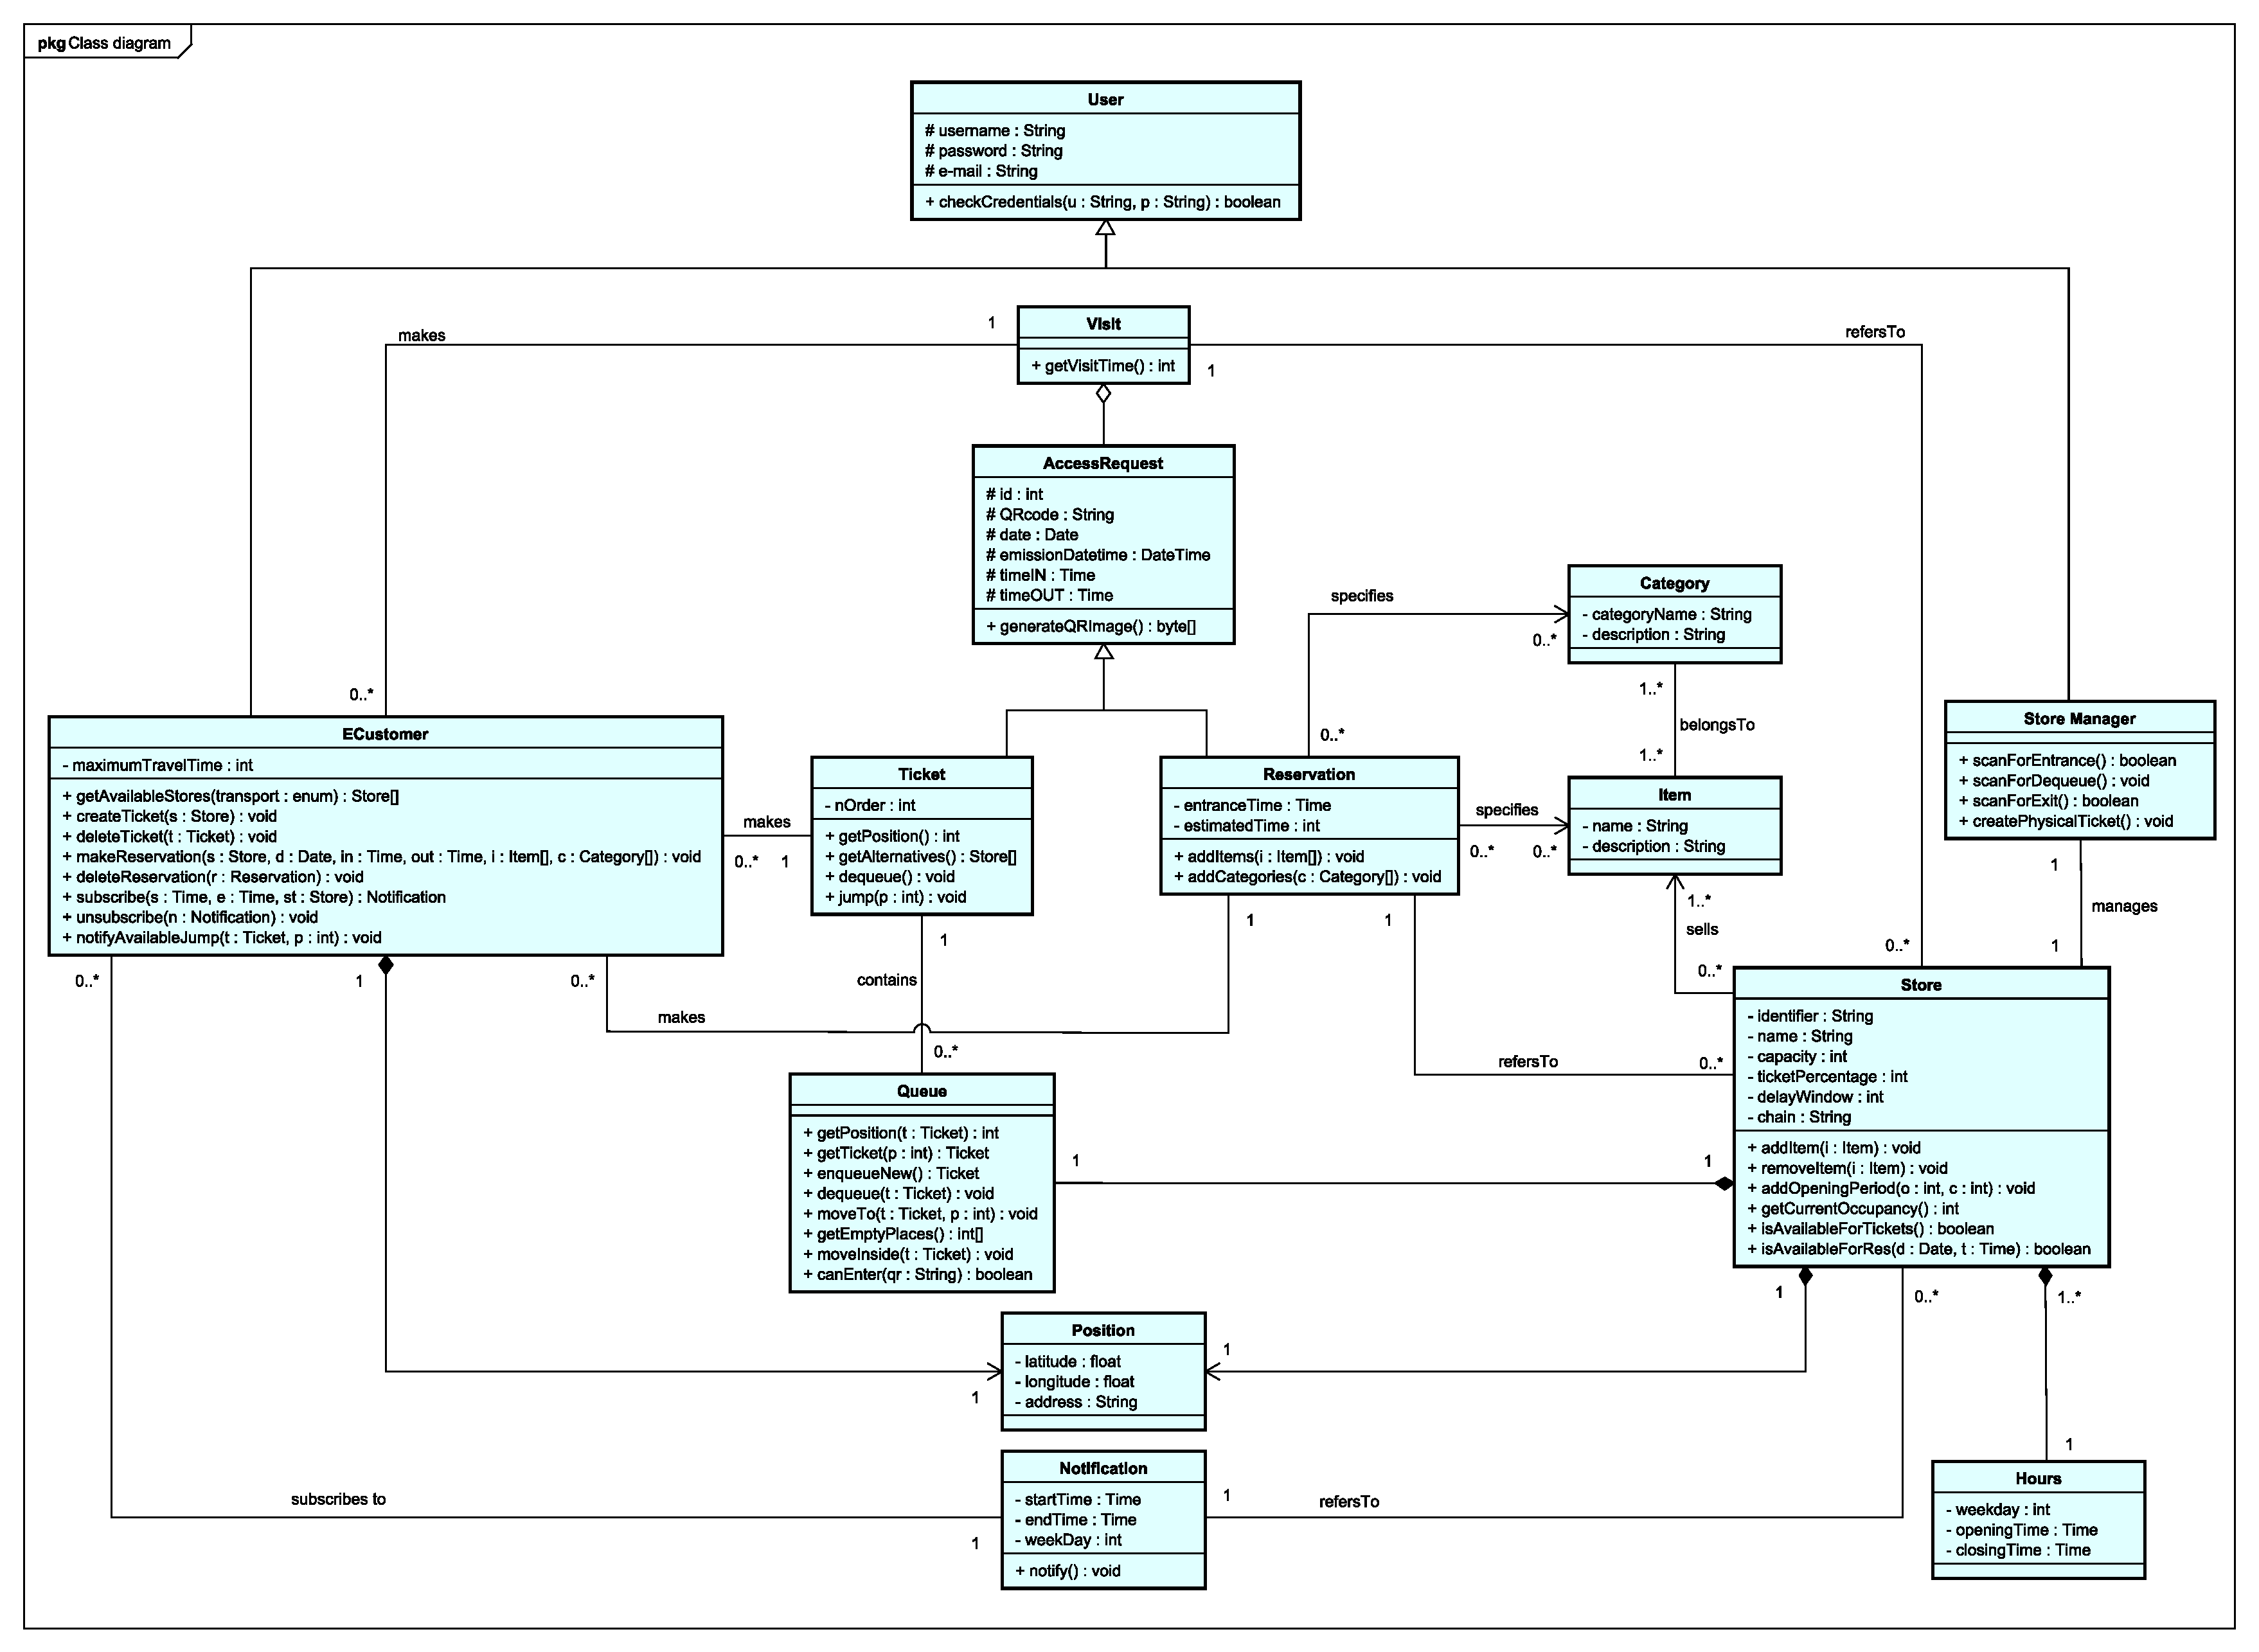
\includegraphics[height=\textheight] {class_diagram/class_diagram}
		\caption{Class Diagram}
		\label{class} 
	\end{figure}
\end{landscape}

\begin{figure}[p]	
	\centering
	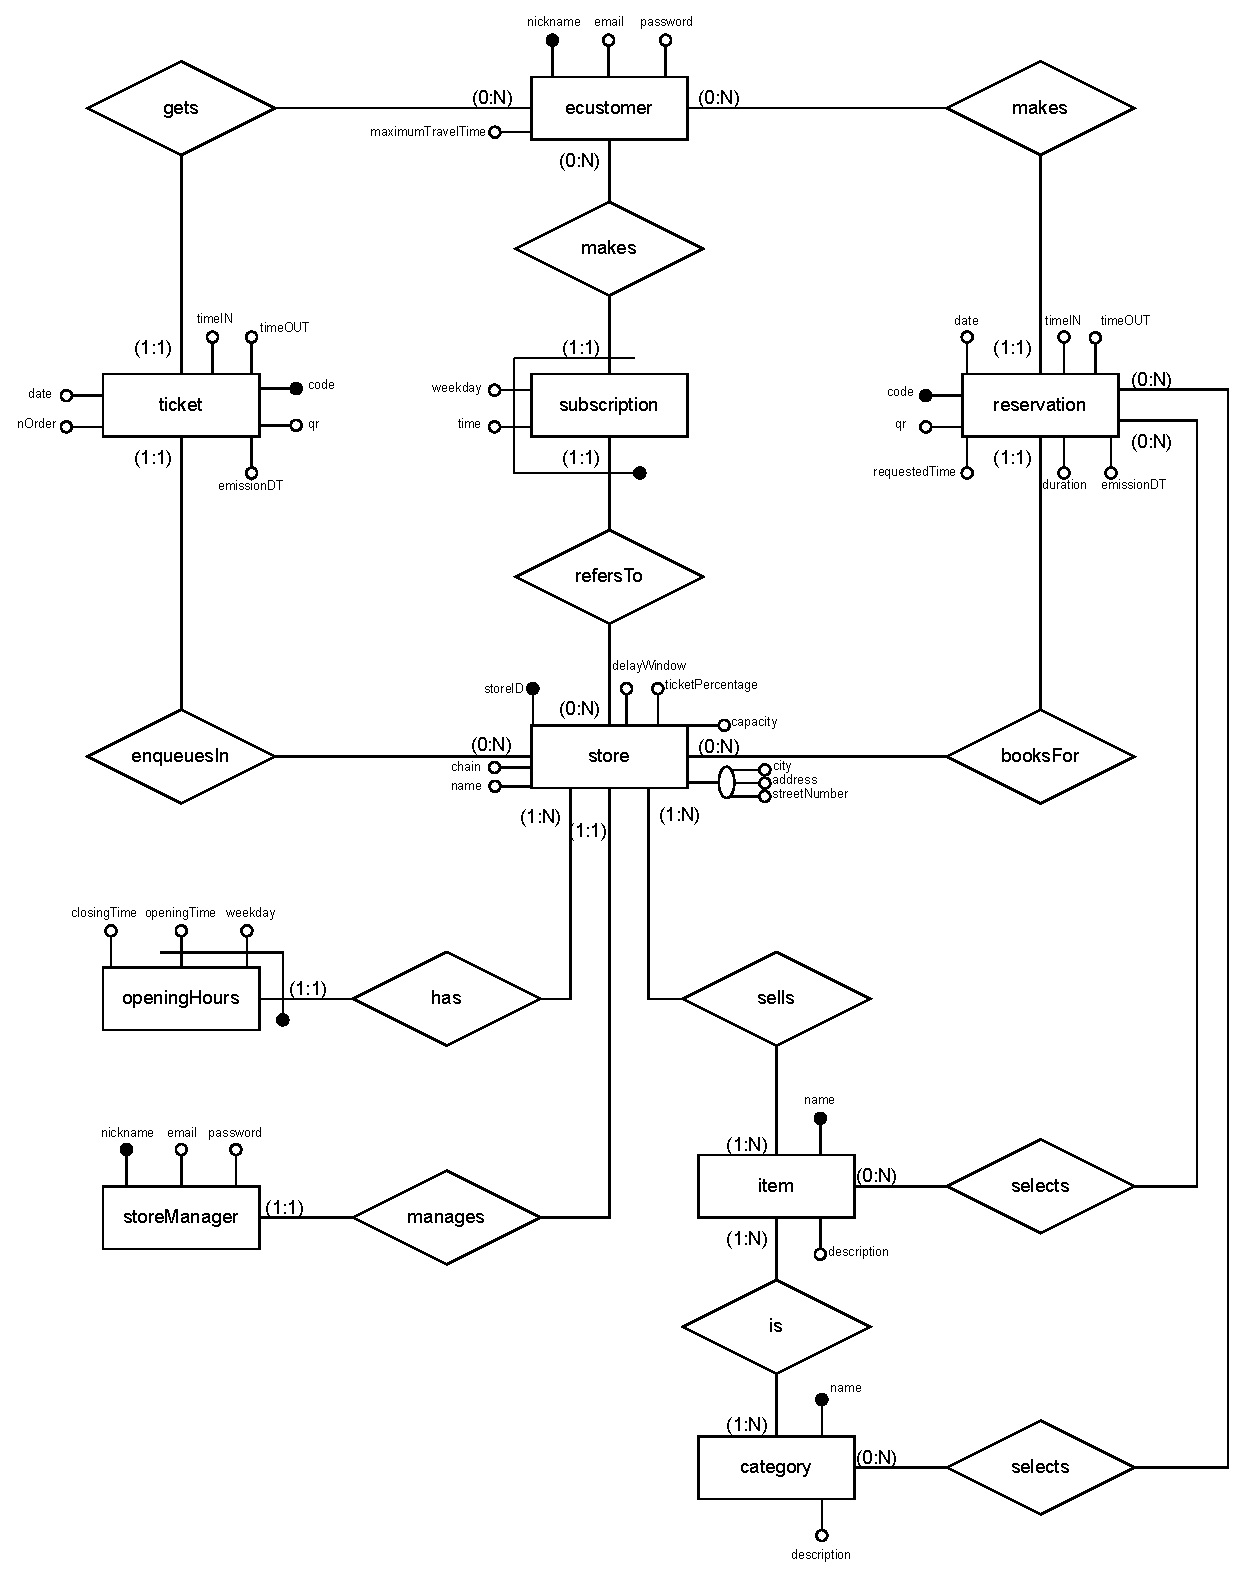
\includegraphics[width=\linewidth] {er_diagram/ERDiagram}
	\caption{ER diagram of the database}
	\label{er} 
\end{figure}
\clearpage
% Component view subsection, to be included in architecture.tex

\subsection{Component view}
This section illustrates the components of the application. Figure \ref{highcomp} offers an high-level representation of the web application's modules; to keep the scheme as clear as possible and avoid modules duplication (which can result misleading), the mobile application module has been omitted, as it connects exactly like the webapp's one. The next sections offer a greater detail on the subsystems, while the components shown here are:

\begin{itemize}[itemsep=-1mm, topsep=-1mm]
	\item Maps Adapter: component used to interface the application with the mapping service's API
	\item Data Access Module: represents the system used to query the relational database 
\end{itemize}

\begin{figure}[h]	
	\centering
	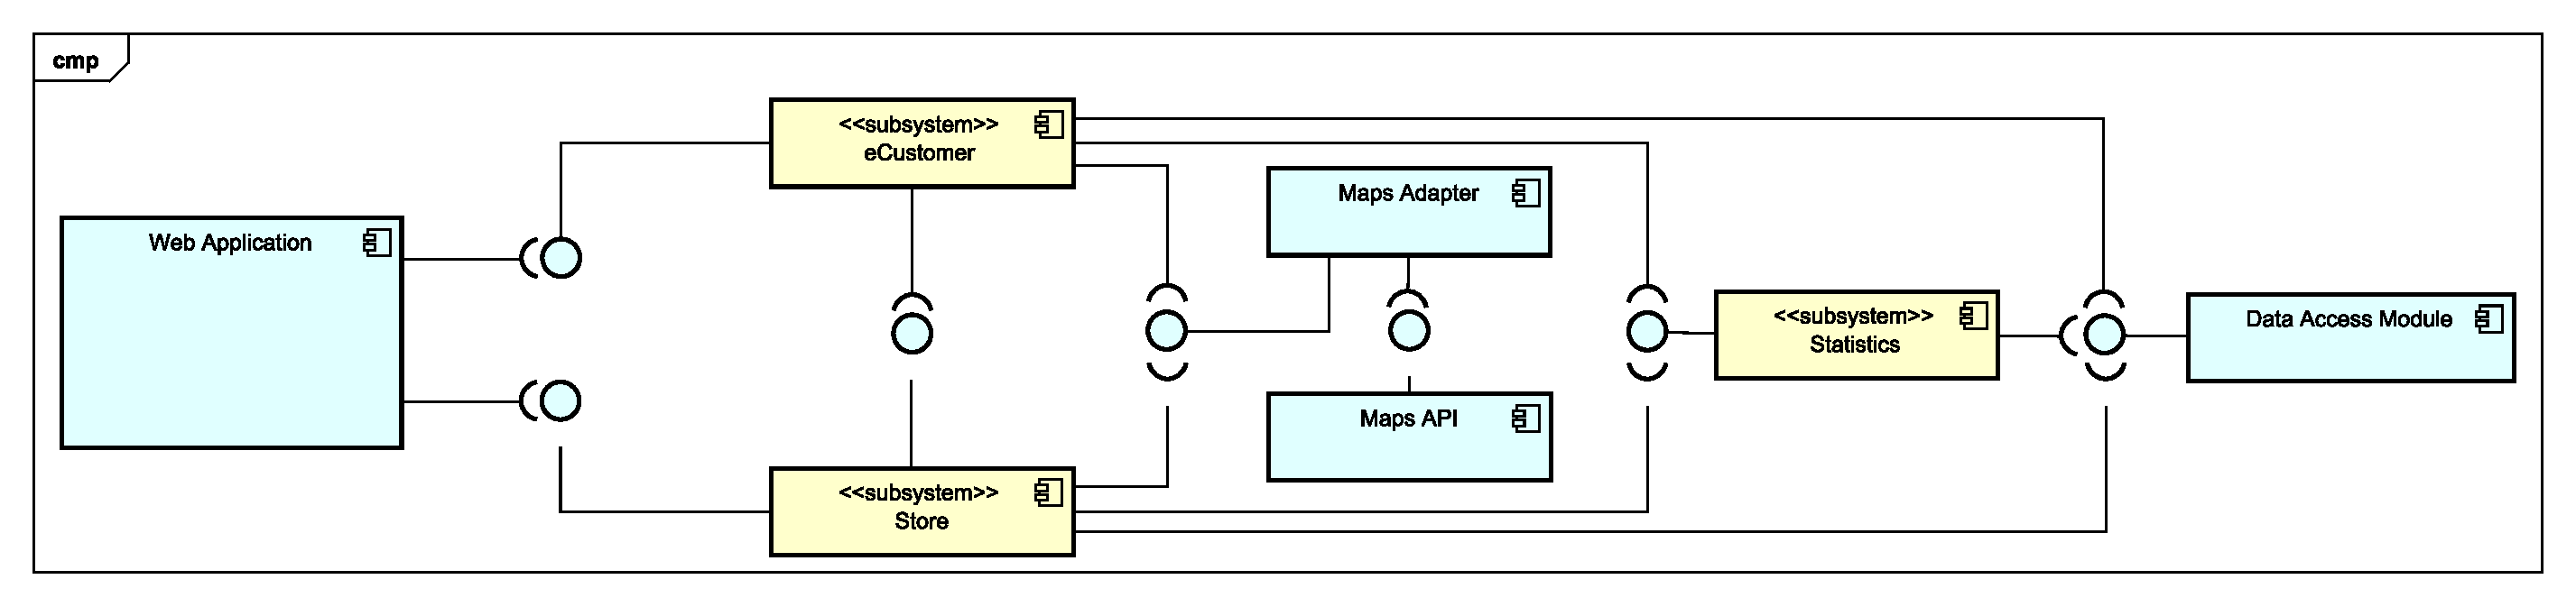
\includegraphics[width=\linewidth] {component_diagrams/component_high}
	\caption{High-level component view}
	\label{highcomp} 
\end{figure}

\subsubsection{Store subsystem}
The store subsystem modules, as shown in Figure 5, are the following:
\begin{itemize}[itemsep=-1mm, topsep=-1mm]
	\item SM Account Manager Module: allows to modify information related to the Store Manager's account
	\item Store Info Manager Module: enables the insert and update of data related to the store (capacity, delay window, items...)
	\item Access Creation Module: controls the creation of reservations and tickets (including the printing of physical ones)
	\item Queue Manager Module: manages a queue of tickets, allowing all operations such as enqueue and dequeue
	\item Visit Manager Module: is responsible for creating visits, scheduling entrances, handle delays, scan codes and manage the customers inside 
\end{itemize}\vspace{.5\baselineskip} 
The connections from components to the Account Manager to check if the Store Manager is logged in are omitted to avoid cluttering, as many modules need to check if the user can access their functions.

\subsubsection{e-Customer subsystem}
The components that realize the e-Customer subsystem are shown in Figure \ref{ecc}. They are:
\begin{itemize}[itemsep=-1mm, topsep=-1mm]
	\item eC Account Manager Module: allows the modification of the e-Customer's profile
	\item Store Recommender Module: manages the retrieval and proposal of stores to the e-Customer; considers location, travel time and store state to create its lists
	\item Access Request Module: is the module responsible for requesting the creation of tickets and reservations and handles the user interaction
	\item Requests Manager Module: controls the visualization and deletion of active tickets and reservations
	\item Notification Module: sends all notifications to the e-Customer when requested by other modules
	\item Subscription Module: handles the user's requests for slot notifications 
\end{itemize}\vspace{.5\baselineskip} 
Internal connections to the Account Manager used to check if the e-Customer is logged in are omitted.

\begin{figure}[p]	
	\centering
	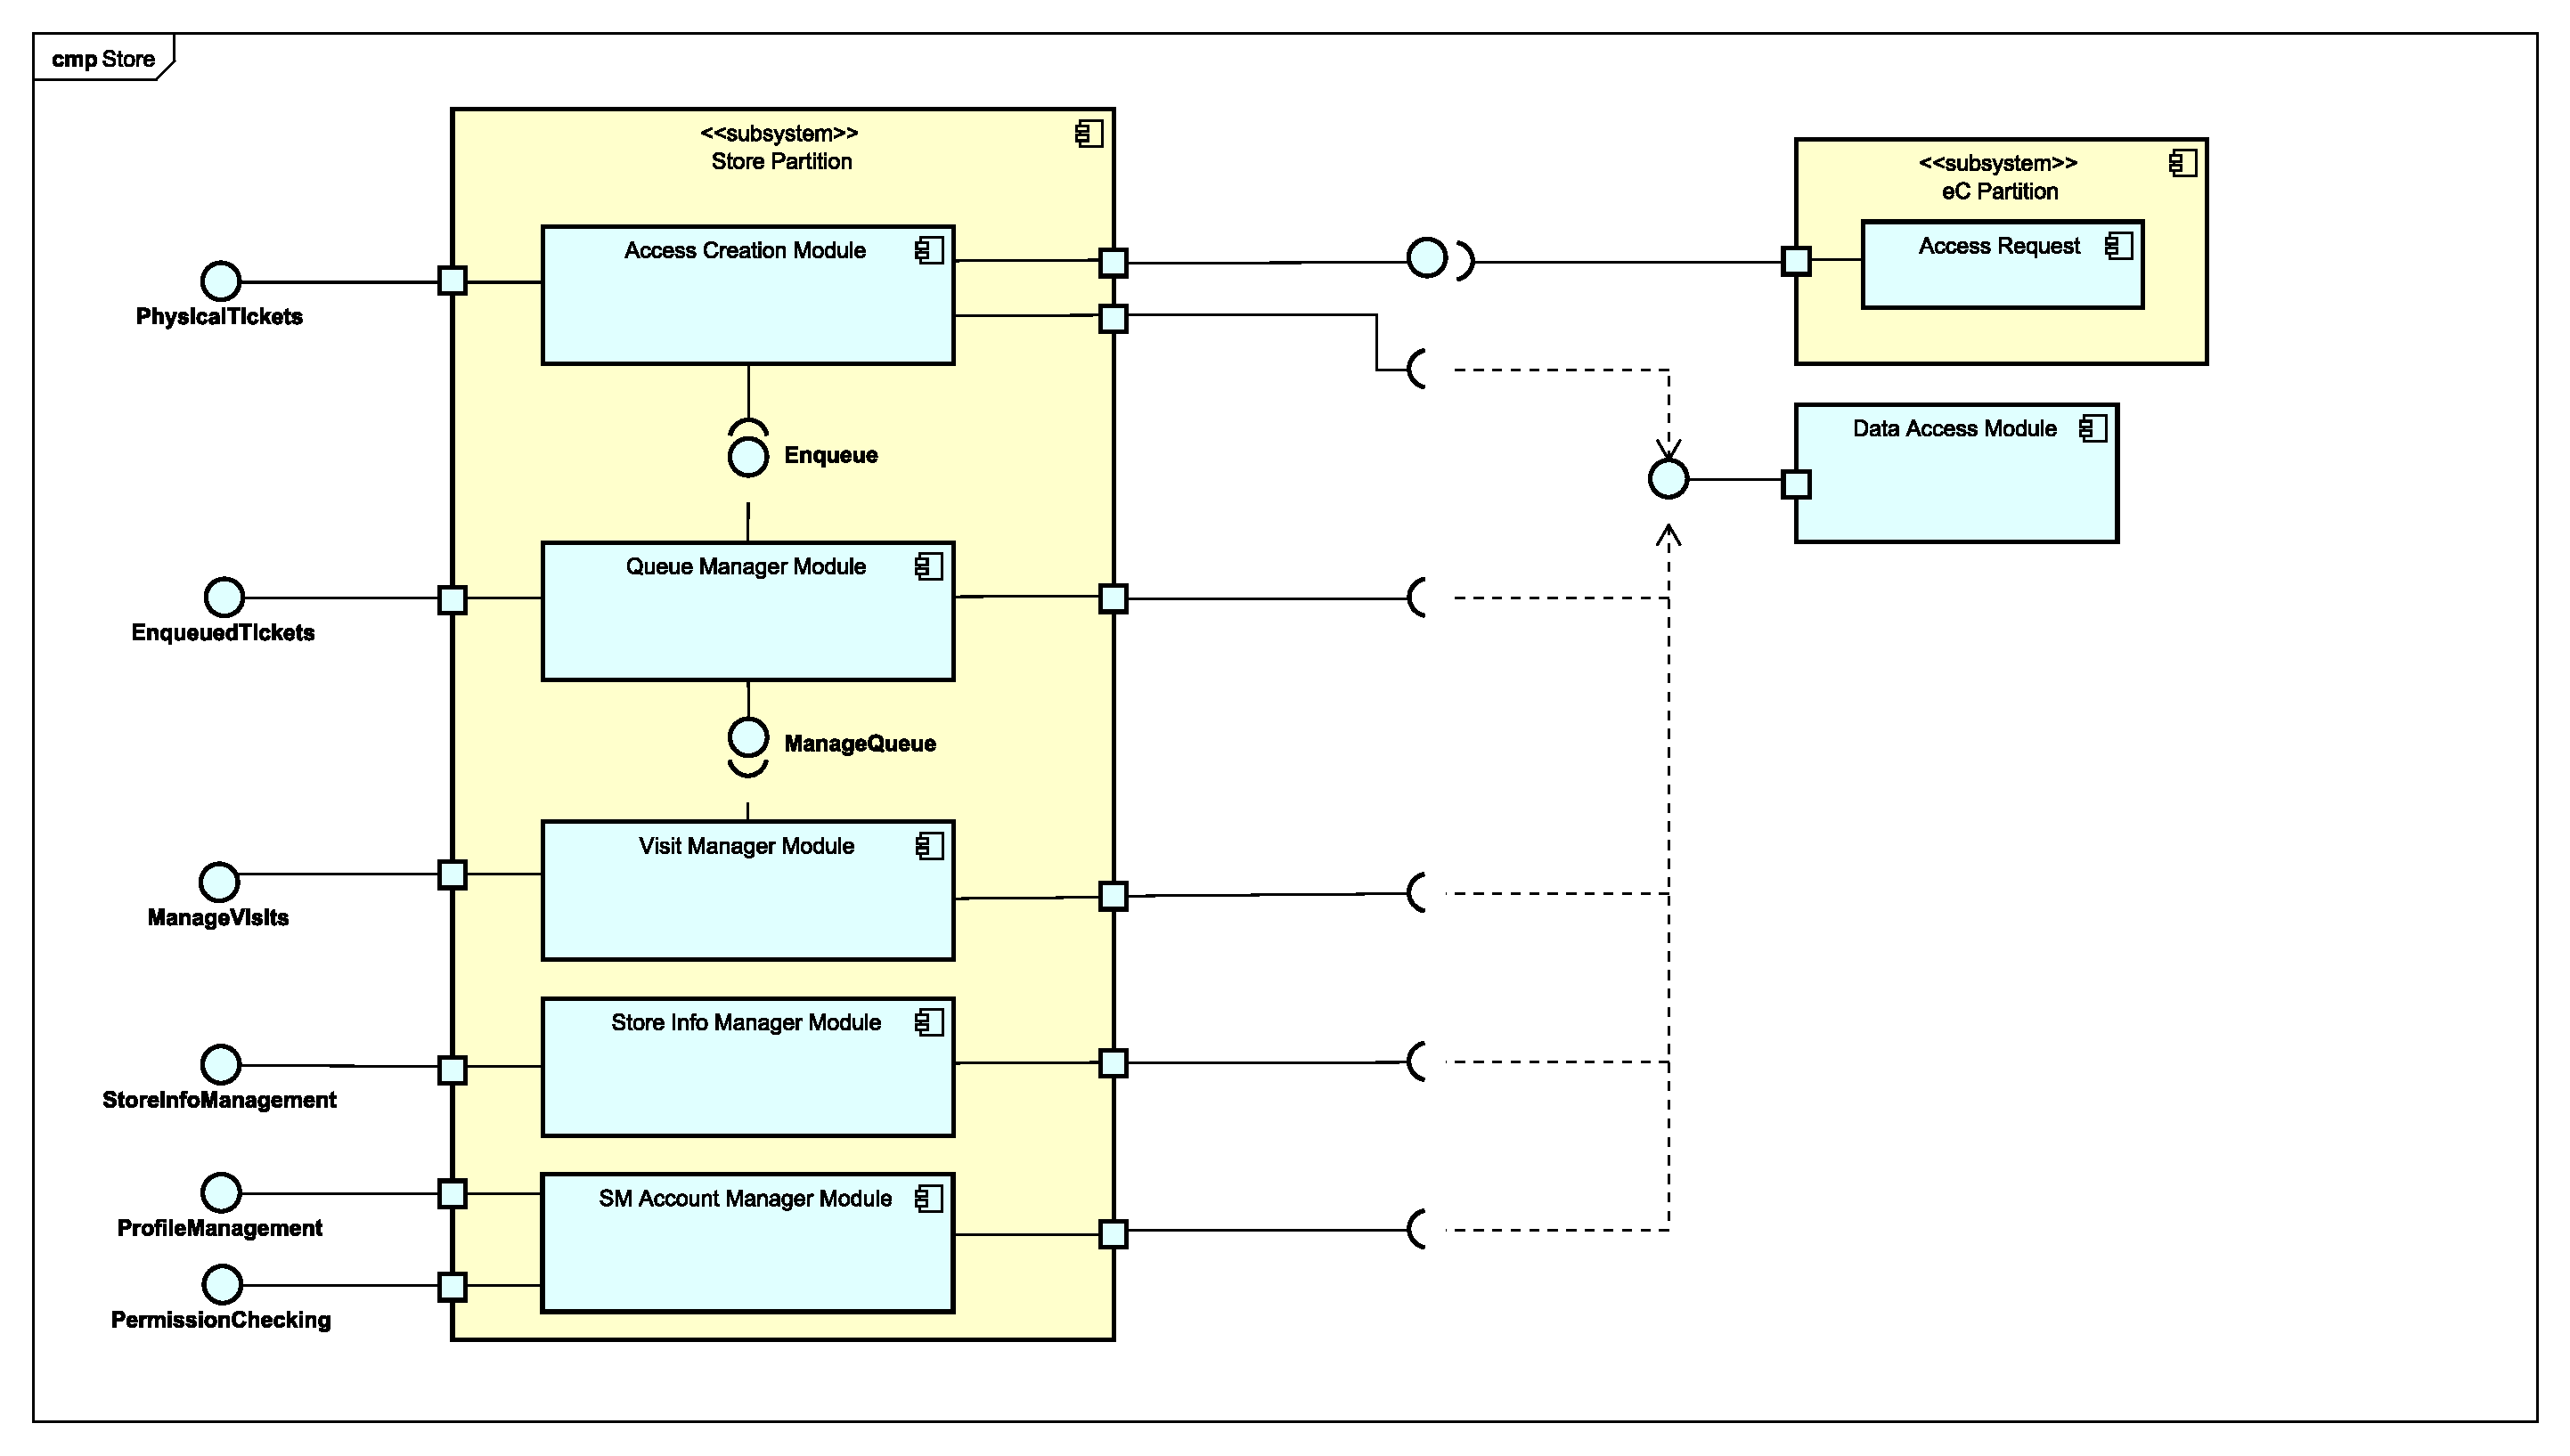
\includegraphics[width=\linewidth] {component_diagrams/component_store}
	\caption{Component view of the Store Manager subsystem}
	\label{smc} 
	
	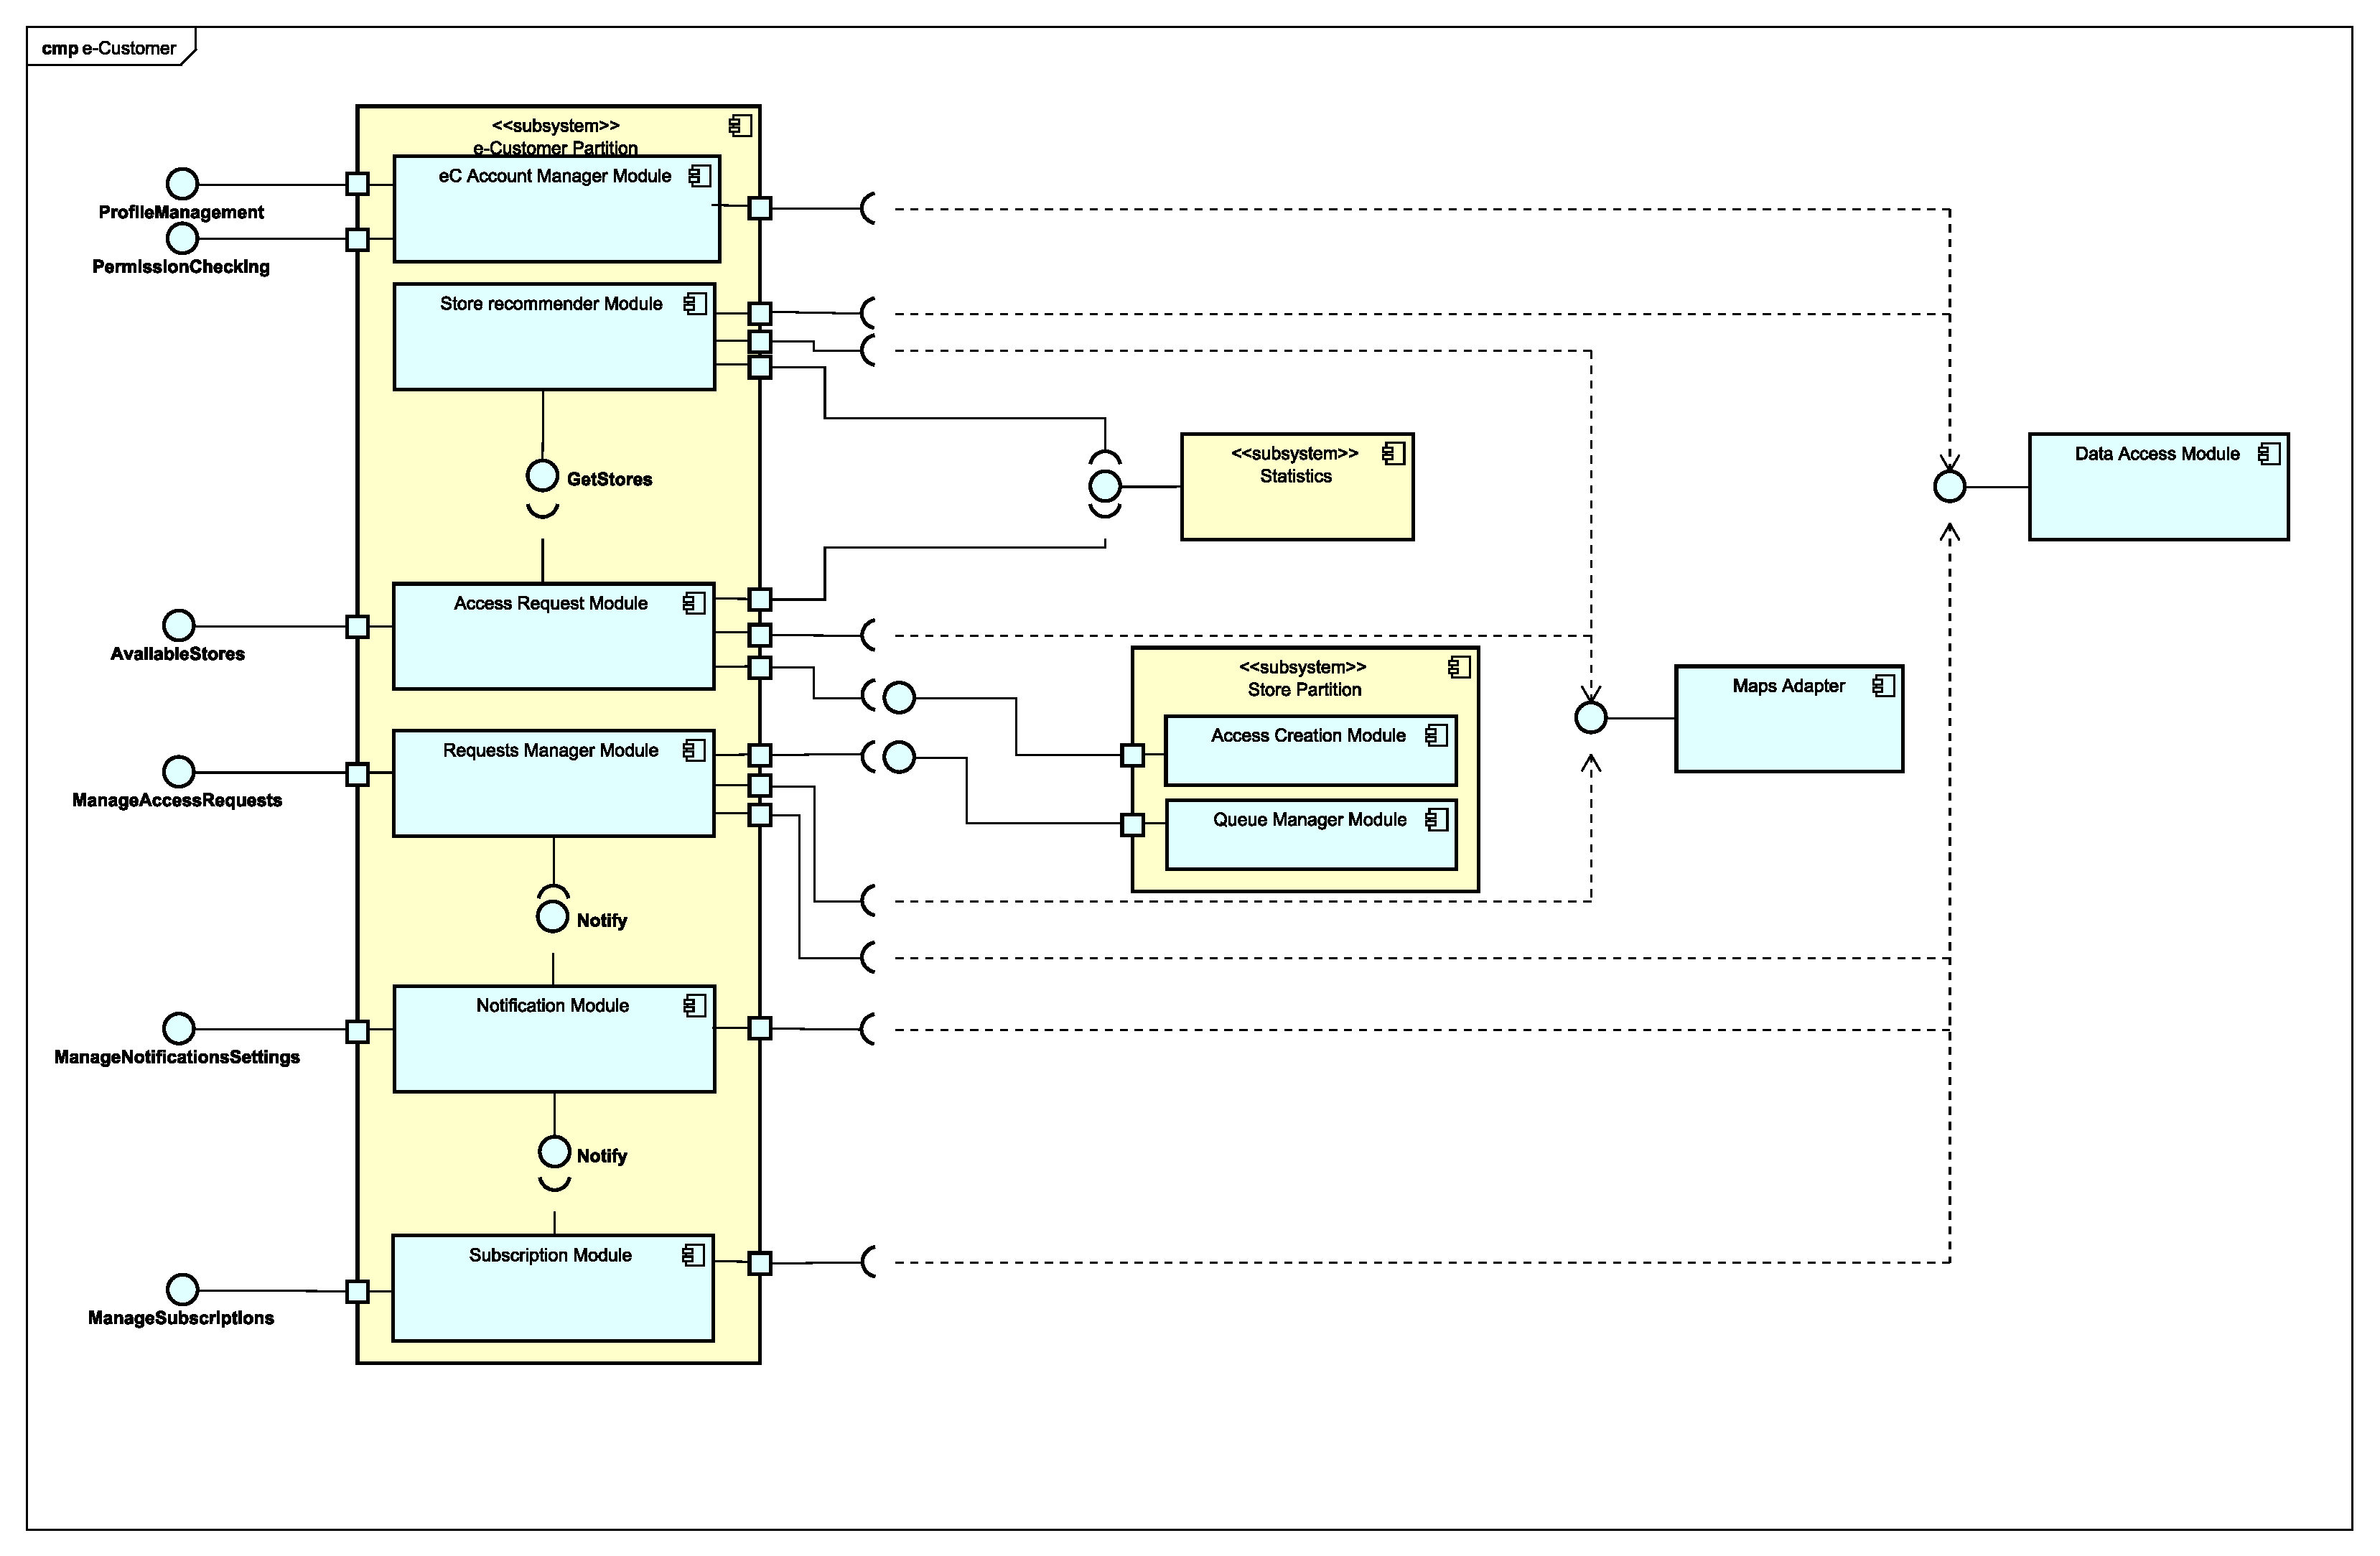
\includegraphics[width=\linewidth] {component_diagrams/component_eC}
	\caption{Component view of the e-Customer subsystem}
	\label{ecc} 
\end{figure}

\subsubsection{Statistics subsystem}
The Statistics subsystem is shown in Figure \ref{stats}. It is composed of:
\begin{itemize}[itemsep=-1mm, topsep=-1mm]
	\item Customer statistics: is responsible for elaborating data such as visit time or preferred store
	\item Store statistics: computes and aggregates data like average time of visit or mean time of queue
\end{itemize}

\begin{figure}[h]	
	\centering
	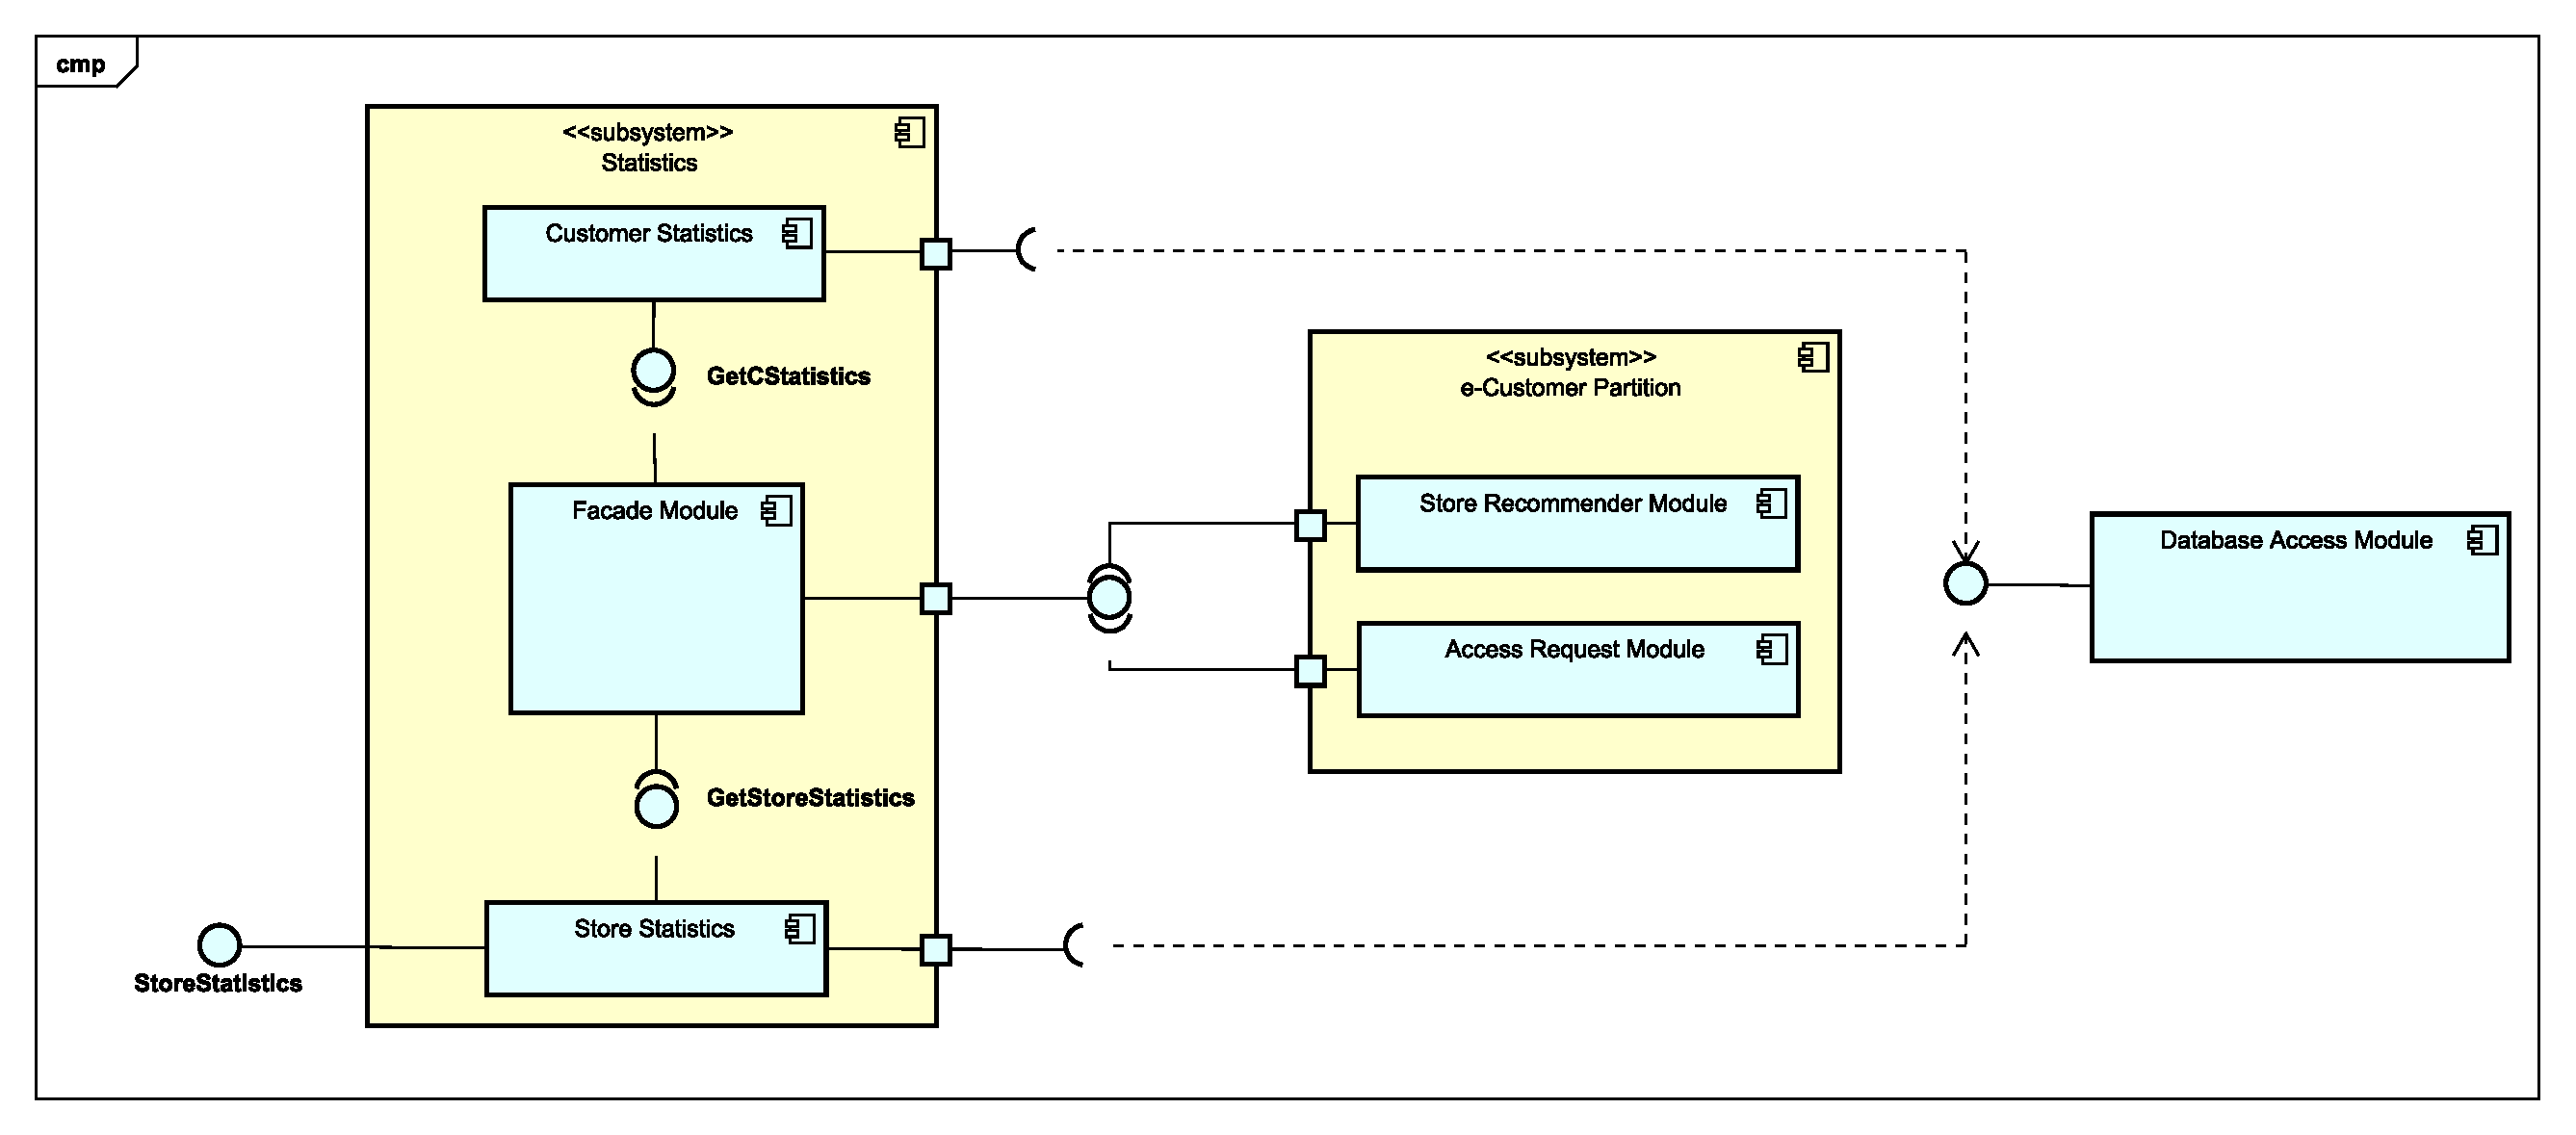
\includegraphics[width=\linewidth] {component_diagrams/statistics}
	\caption{Component view of the Statistic subsystem}
	\label{stats} 
\end{figure}

% Deployment view subsection, to be included in architecture.tex

\subsection{Deployment view}
\label{sect:deploy}
The deployment view of the application can be seen in Figure \ref{deploy}. 
It uses a 5-tier architecture to separate the web aspects from the application itself and from the data. This way, the code can be better decomposed to increase reusability and for security reasons, exposing only the web tier to browsers. The safety of the system is ensured by the use of two DMZs, one isolating the web tier from the rest and one to better protect the data layer. 

With respect to the theoretical layer subdivision, layers 2 and 3 have been united through the use of Apache Tomcat, that covers both the web server's and servlet container's functions.

\begin{landscape}
	\begin{figure}[p]
		\centering	
		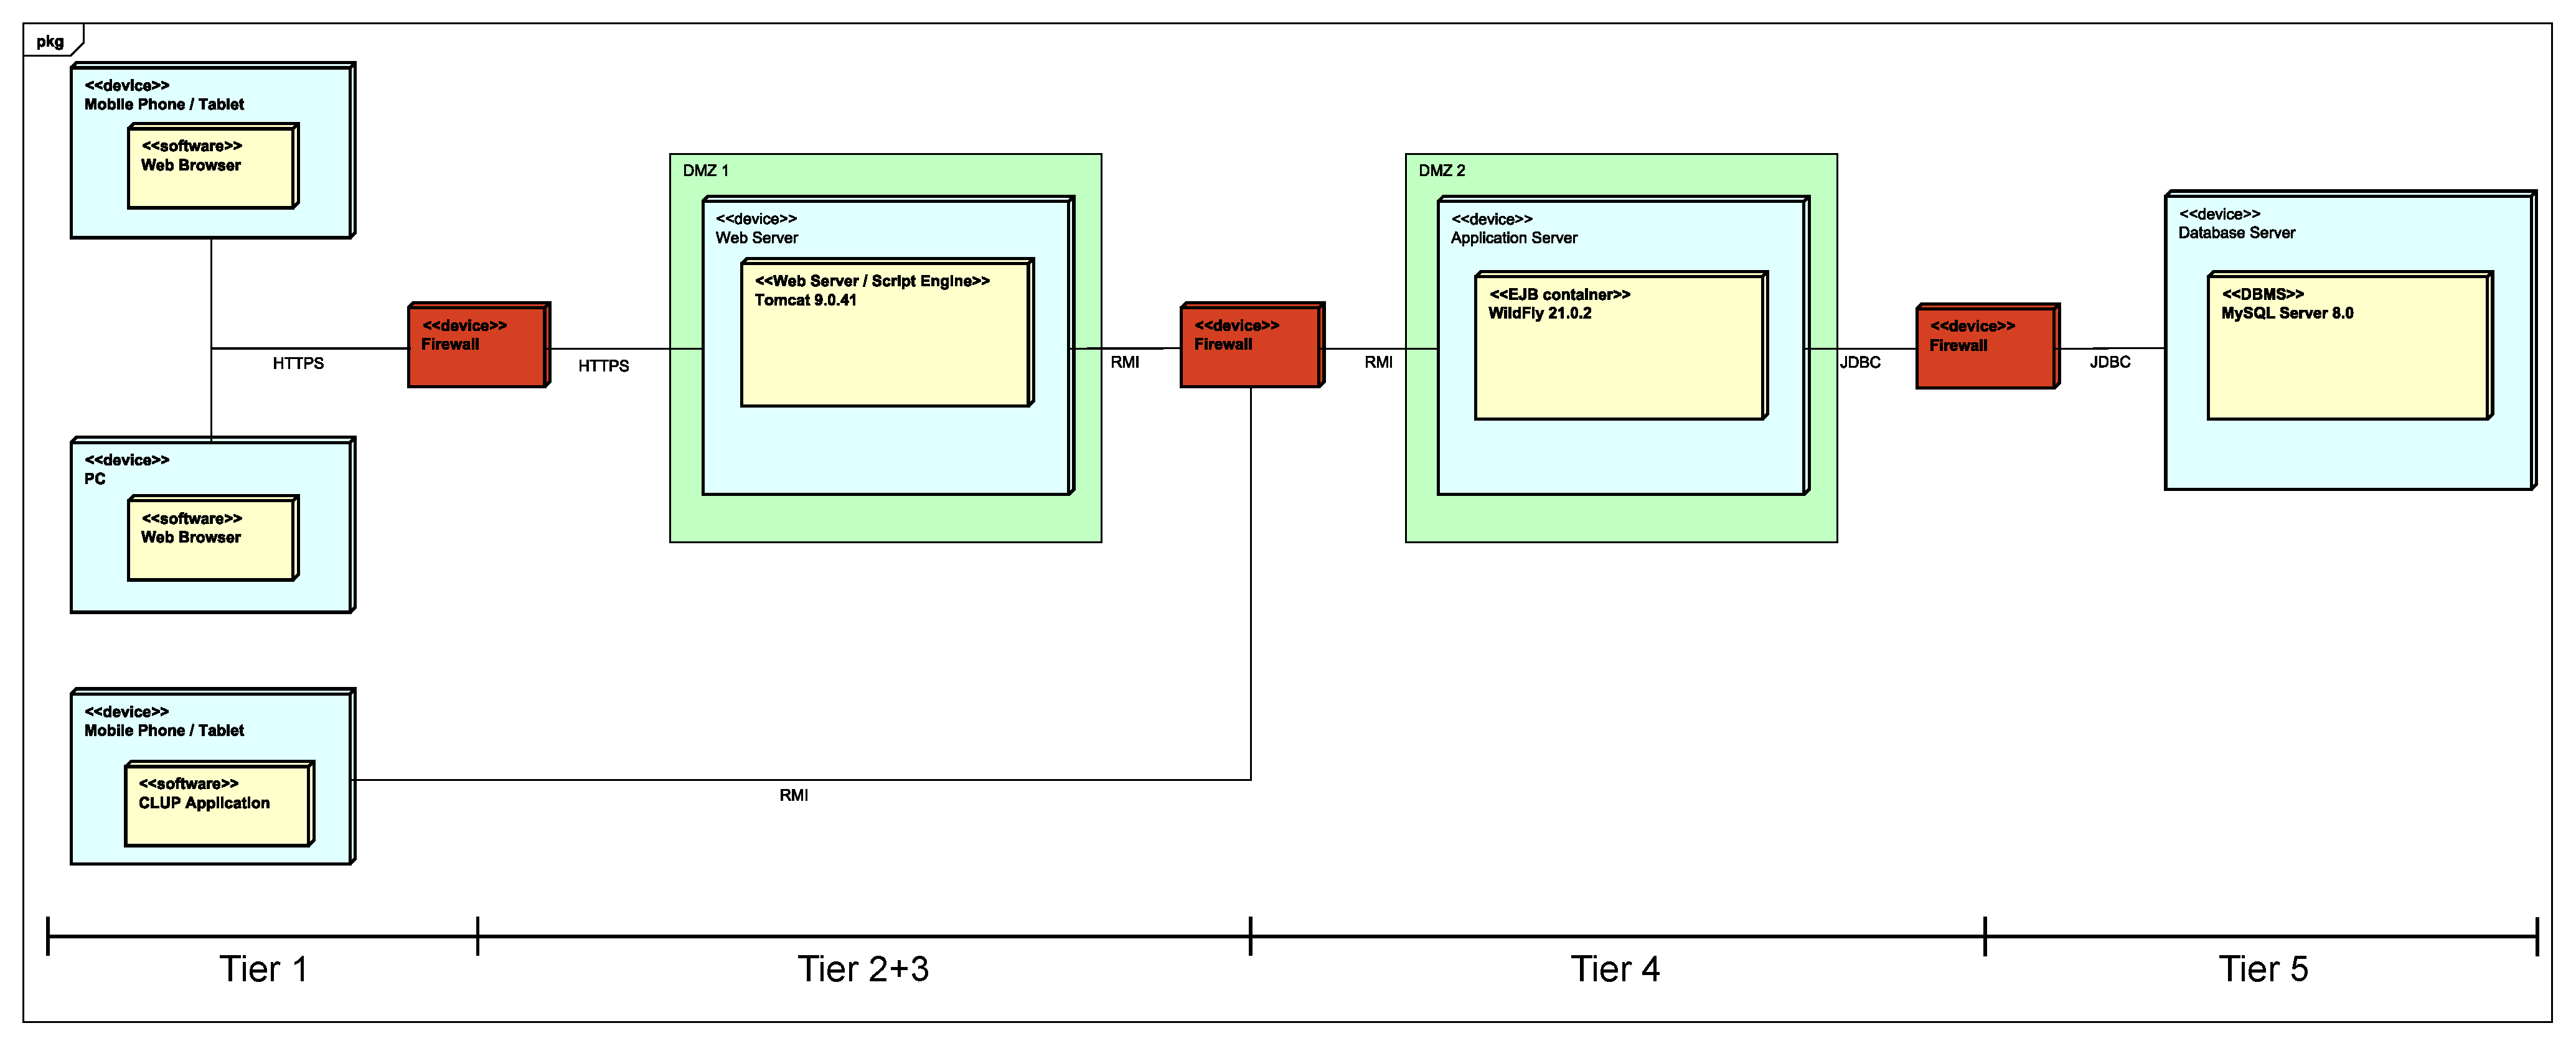
\includegraphics[width=\linewidth] {deployment_diagrams/deployment}
		\caption{Deployment diagram of the application}
		\label{deploy} 
	\end{figure}
\end{landscape}

% Runtime view subsection, to be included in architecture.tex

\subsection{Runtime view}
This section covers some of the interactions among the system's components. 

Figure \ref{runeclogin} shows the interaction between modules to achieve the e-Customer login function.

Diagrams in Figures \ref{runecticket} and \ref{runecvisit} represent the different steps needed for getting a ticket or booking a visit for an e-Customer. The core of these processes is the retrieval of stores, done through the following steps:
\begin{itemize}[itemsep=-1mm, topsep=-1mm]
  	\item The Access Request module asks for the localization of the user
  	\item The Store Recommender requests stores close to the user based on the parameters defined by the user (as mean of transport, maximum travel time...)
  	\item The Recommender then queries the database to know which of the candidate stores use CLup
  	\item The returned stores are checked for availability to host more tickets based on the queues and time of visits
  	\item The finally filtered list is then returned to the user
\end{itemize}\vspace{.5\baselineskip}
This order has been defined to offer an incremental filter, allowing to access the maps API only once and limit the accesses to the DB to requests only for previously identified store. Furthermore, the request for stores on a geographic base would be limited anyway even for large cities\textsuperscript{\cite{food}}, as opposed to extracting all stores in the database.

\begin{figure}[h]	
	\centering
	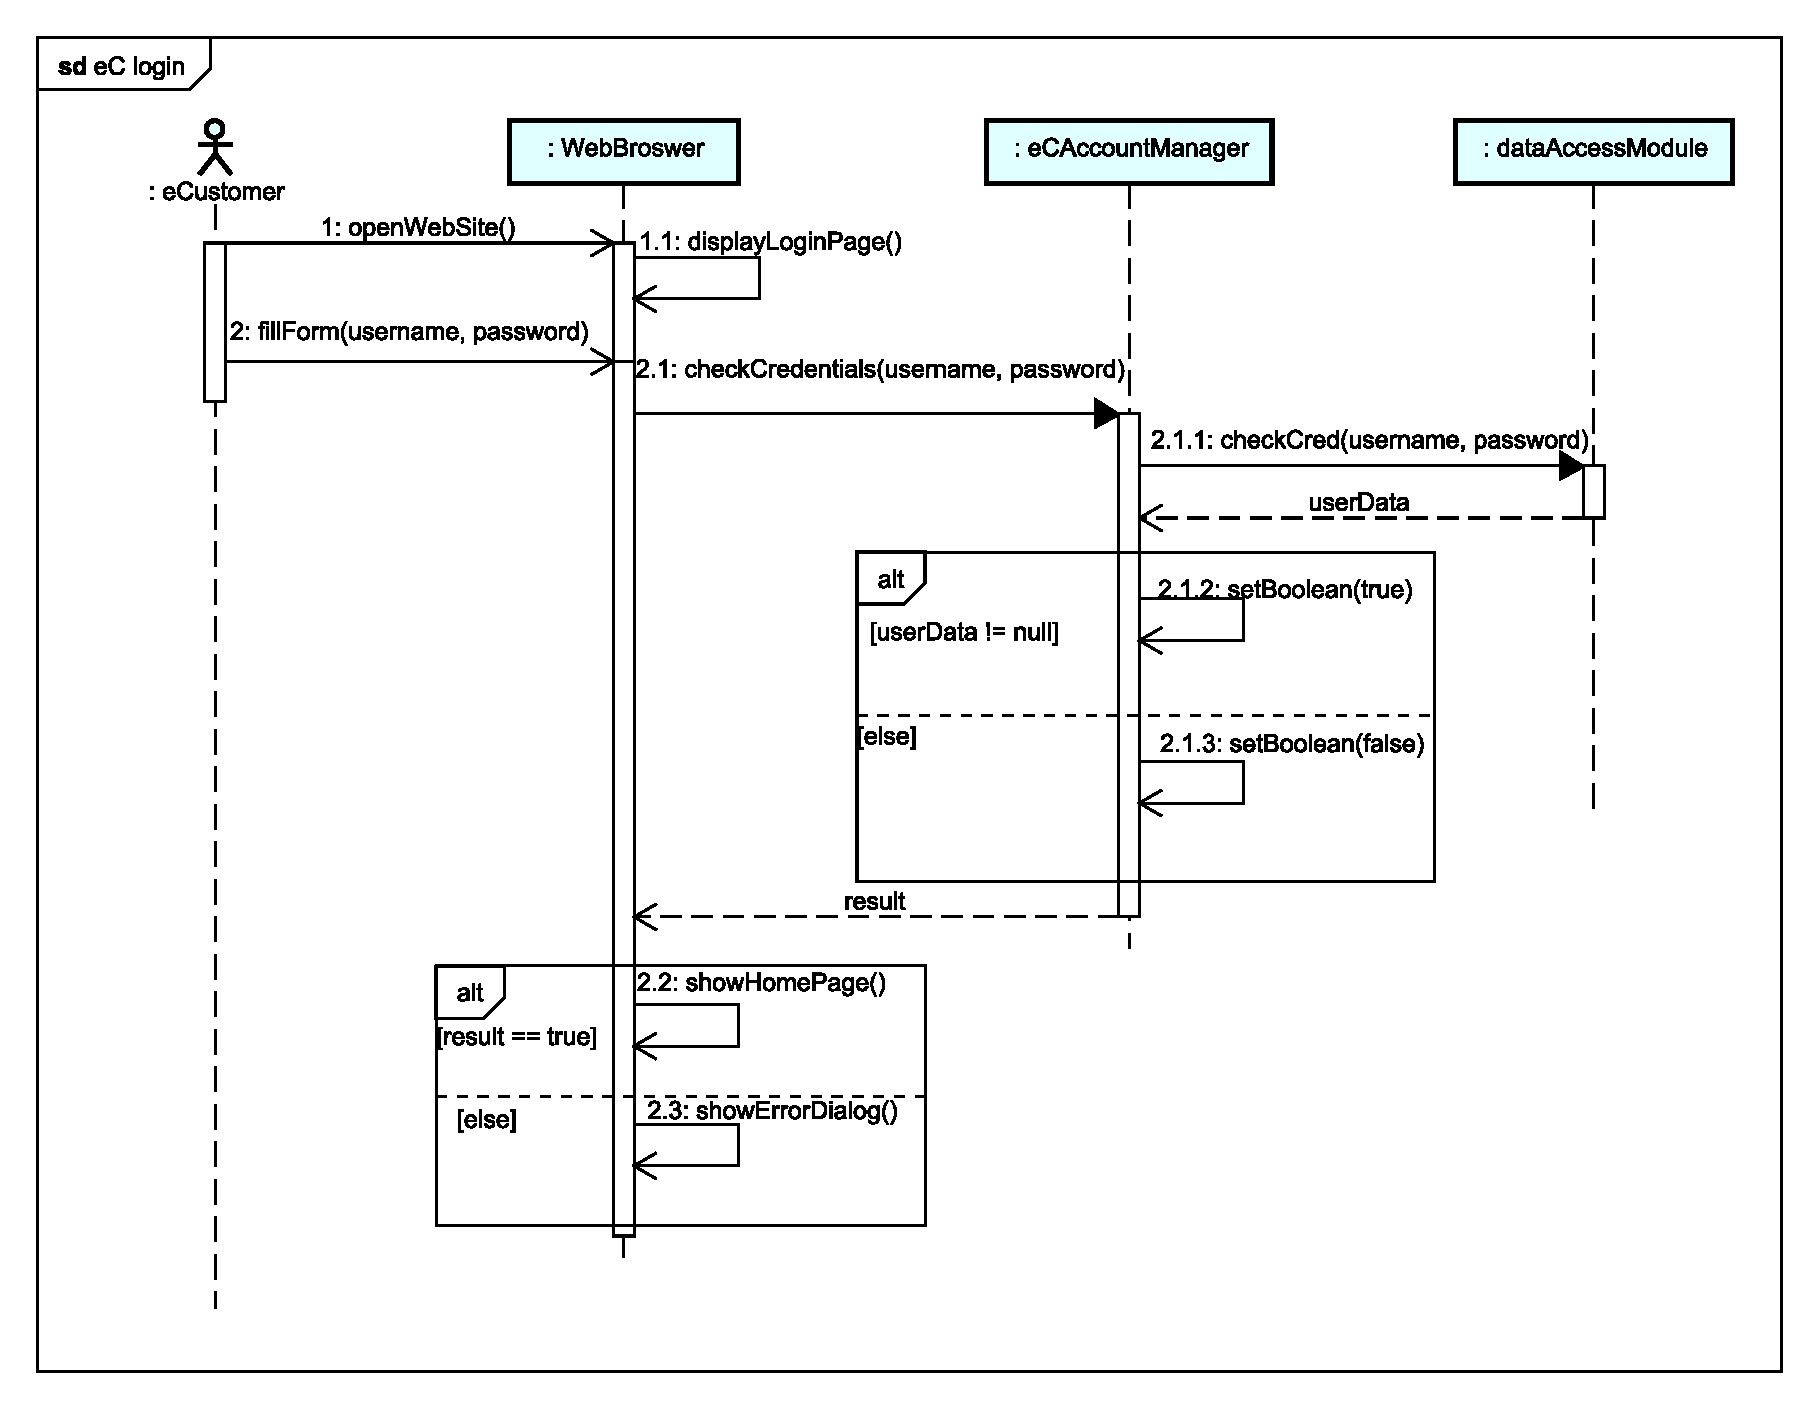
\includegraphics[width=\linewidth] {sequence_diagrams/eC_login_seqD}
	\caption{Runtime view of an e-Customer login}
	\label{runeclogin} 
\end{figure}

\begin{landscape}
	\begin{figure}[p]
		\centering	
		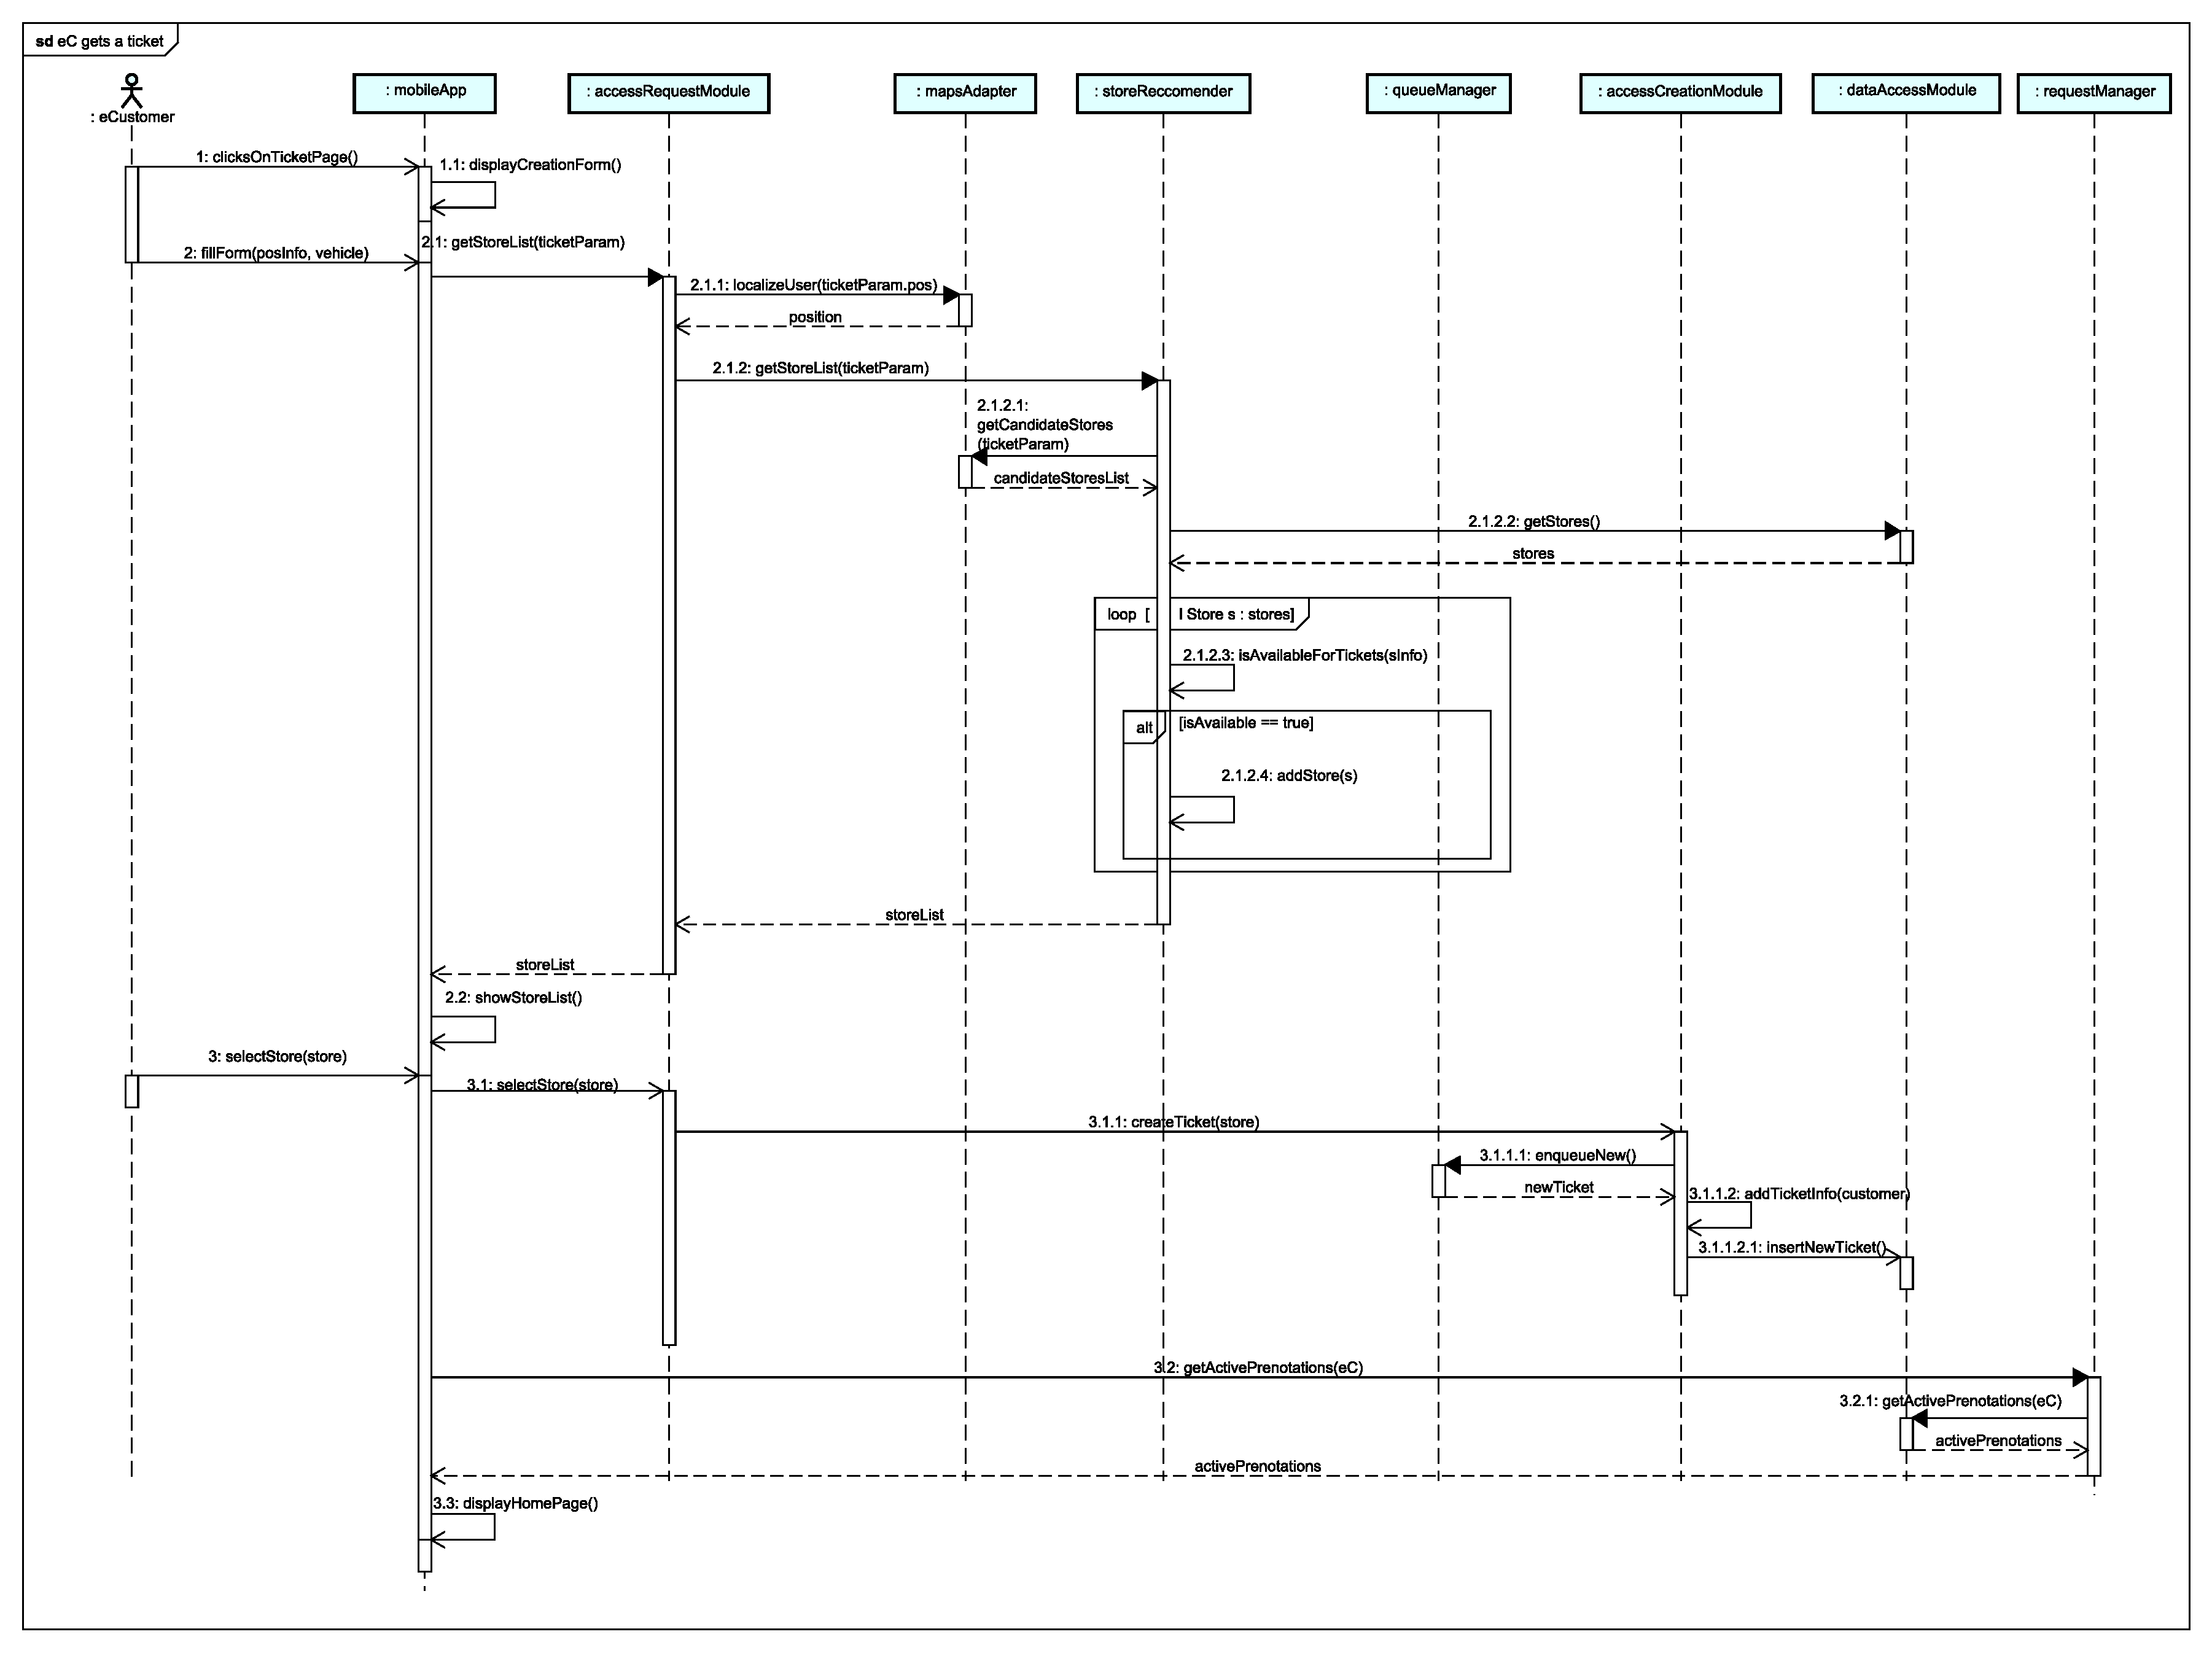
\includegraphics[height=\textheight] {sequence_diagrams/eC_gets_a_ticket_seqD}
		\caption{Runtime view of an e-Customer getting a ticket}
		\label{runecticket} 
	\end{figure}
	
	\begin{figure}[p]
		\centering	
		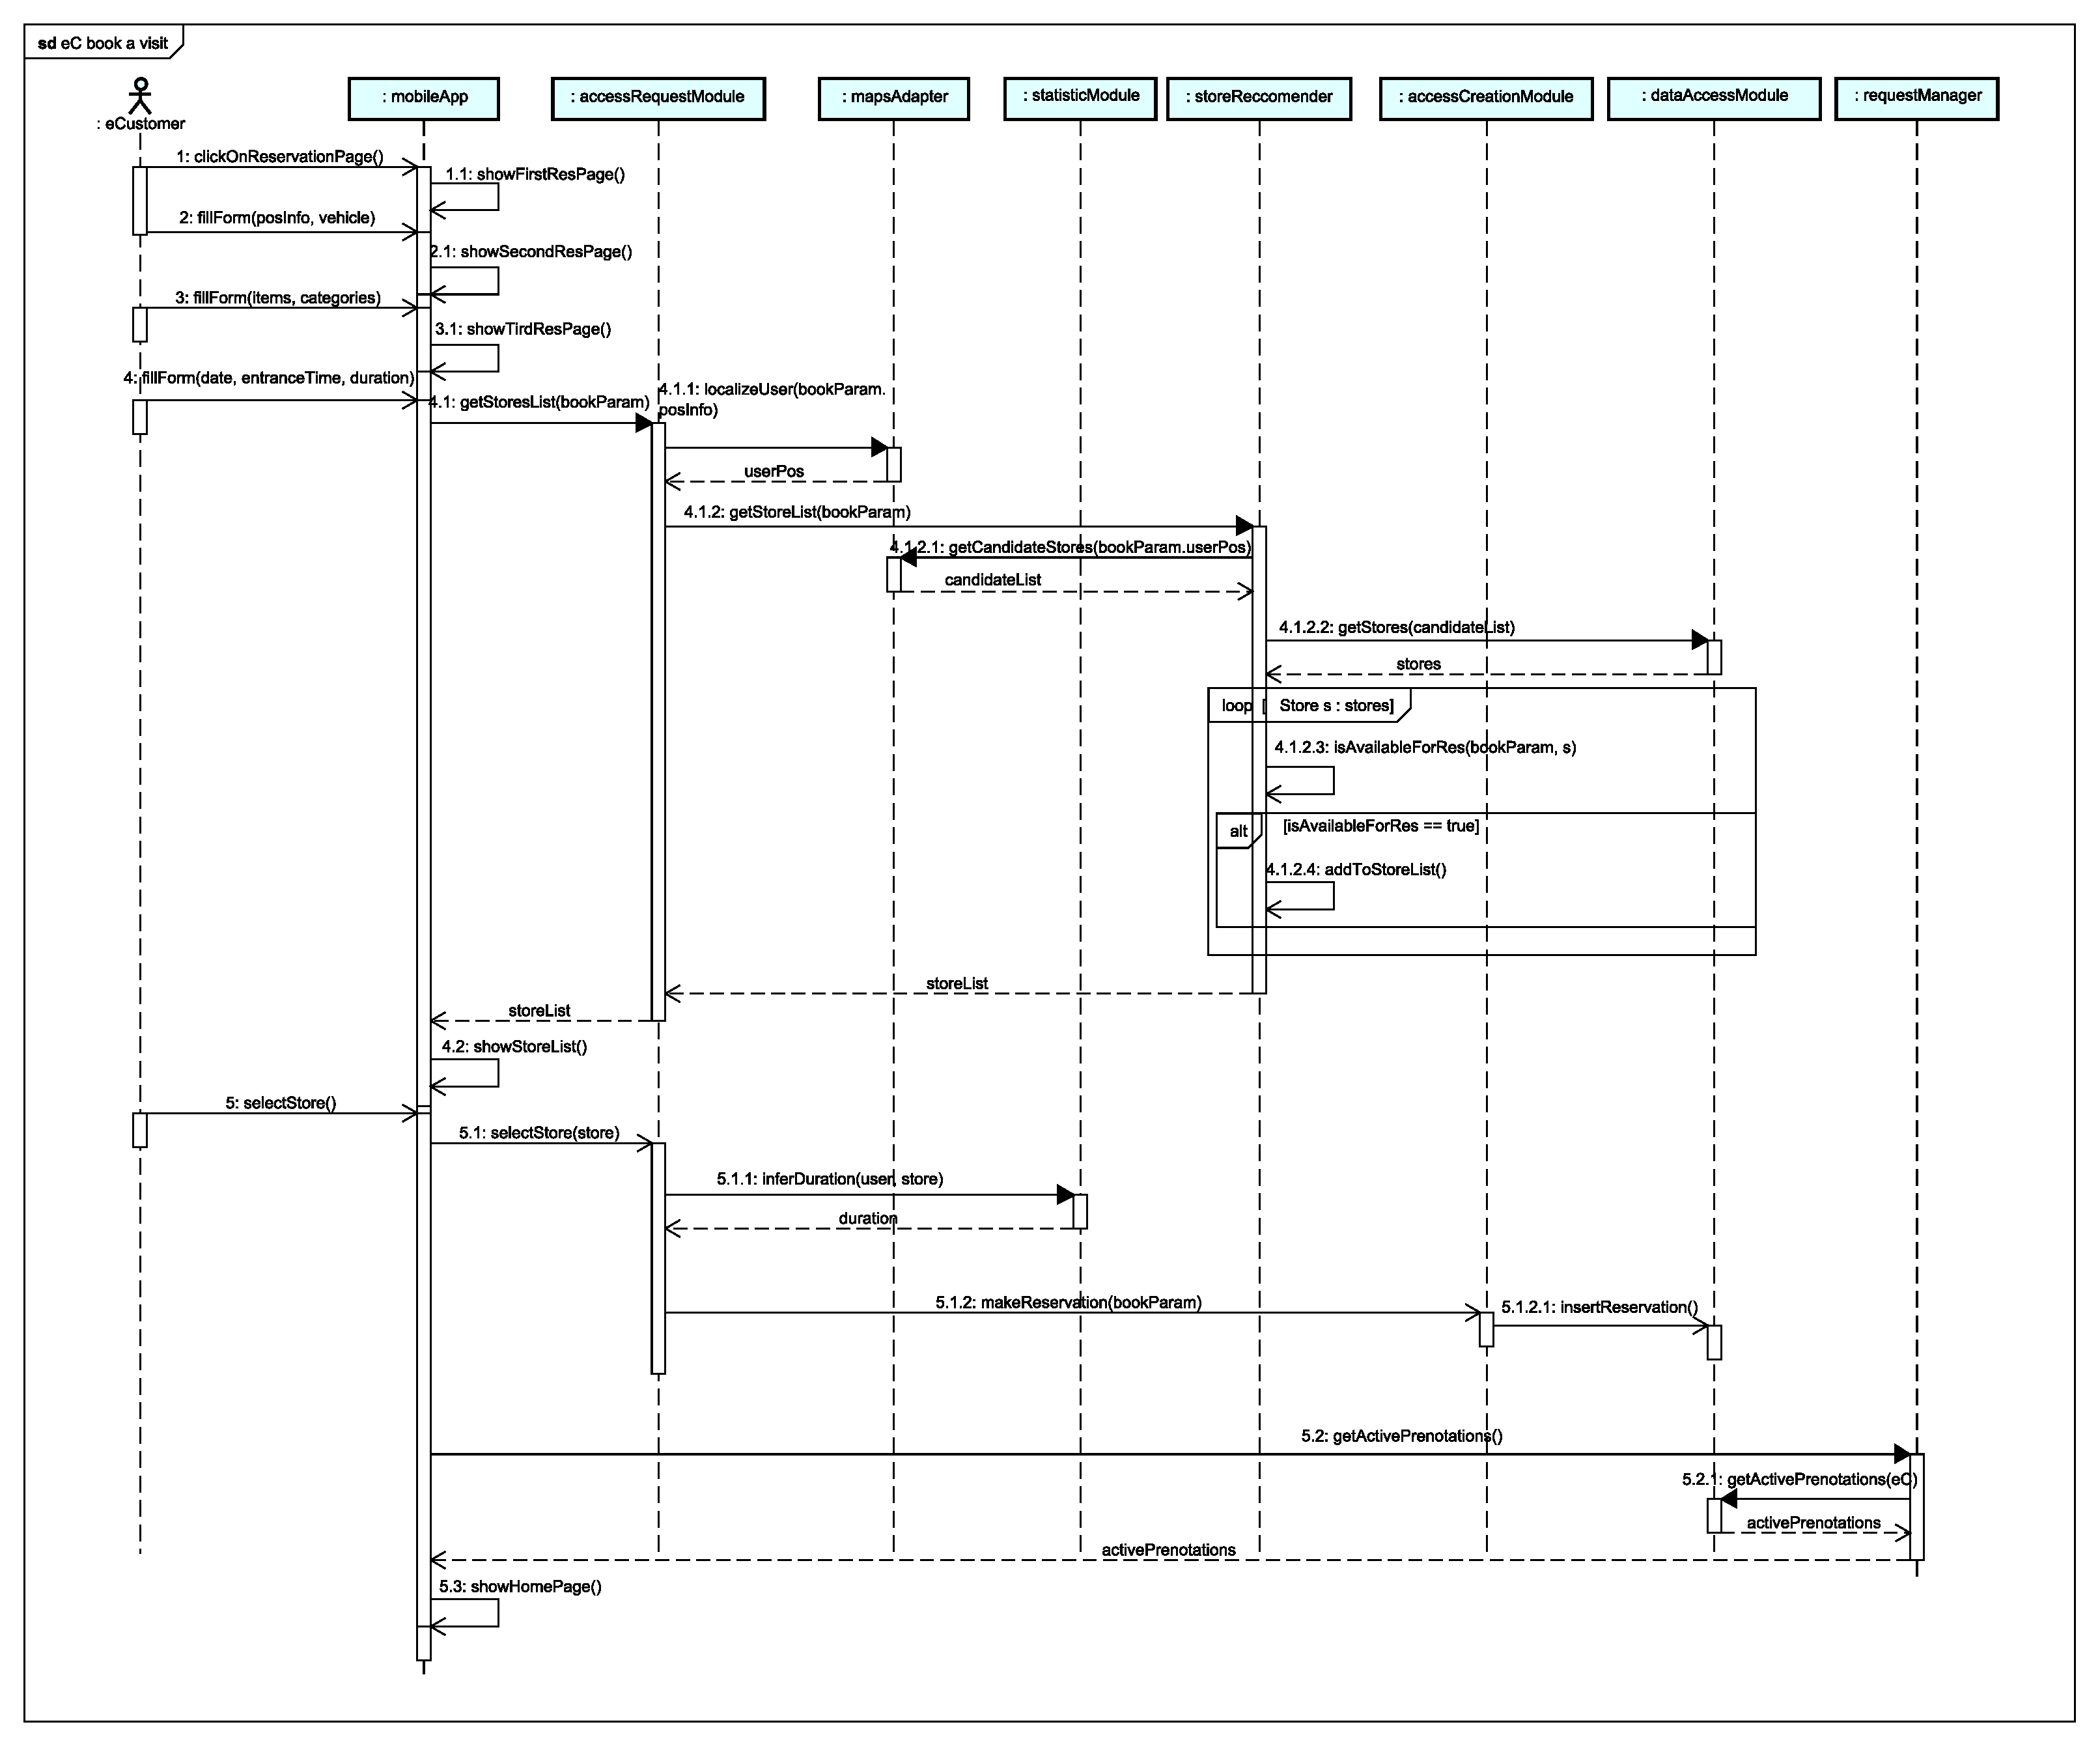
\includegraphics[height=\textheight] {sequence_diagrams/eC_book_a_visit_seqD}
		\caption{Runtime view of an e-Customer booking a visit}
		\label{runecvisit} 
	\end{figure}
\end{landscape}


Figure \ref{ecdelete} illustrates how the request of ticket deletion by an e-Customer is carried out, while Figures \ref{smmodinfo} and \ref{runsmmonitor} concern Store Manager activities, namely modifying their store's information and scanning entering tickets or reservations.

\begin{figure}[h]	
	\centering
	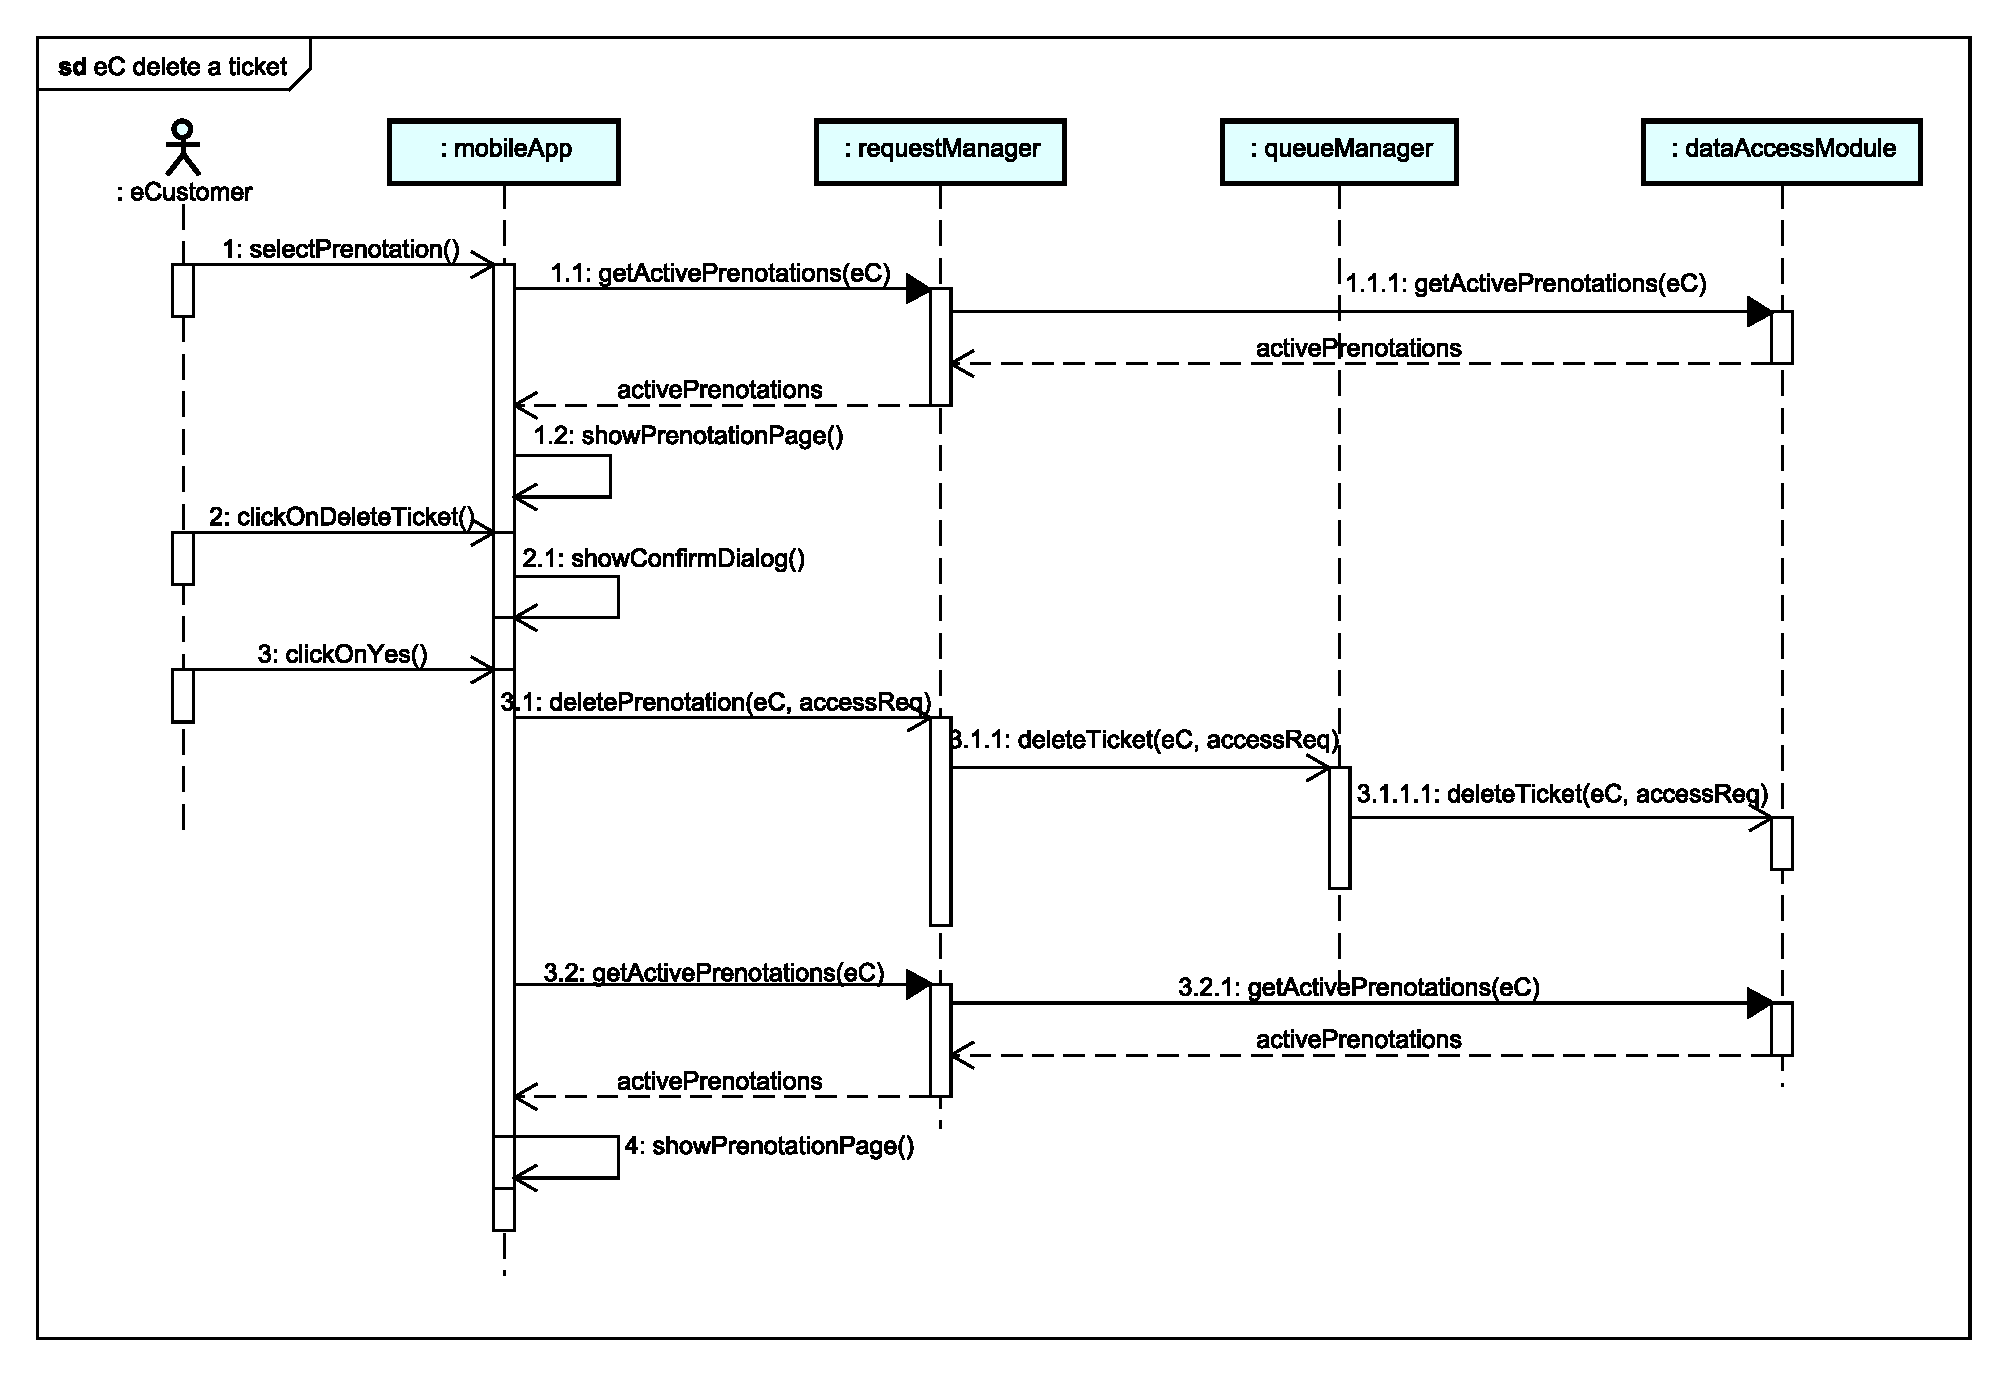
\includegraphics[width=.75\linewidth] {sequence_diagrams/eC_delete_a_ticket_seqD}
	\caption{Runtime view of an e-Customer deleting a ticket}
	\label{ecdelete} 

	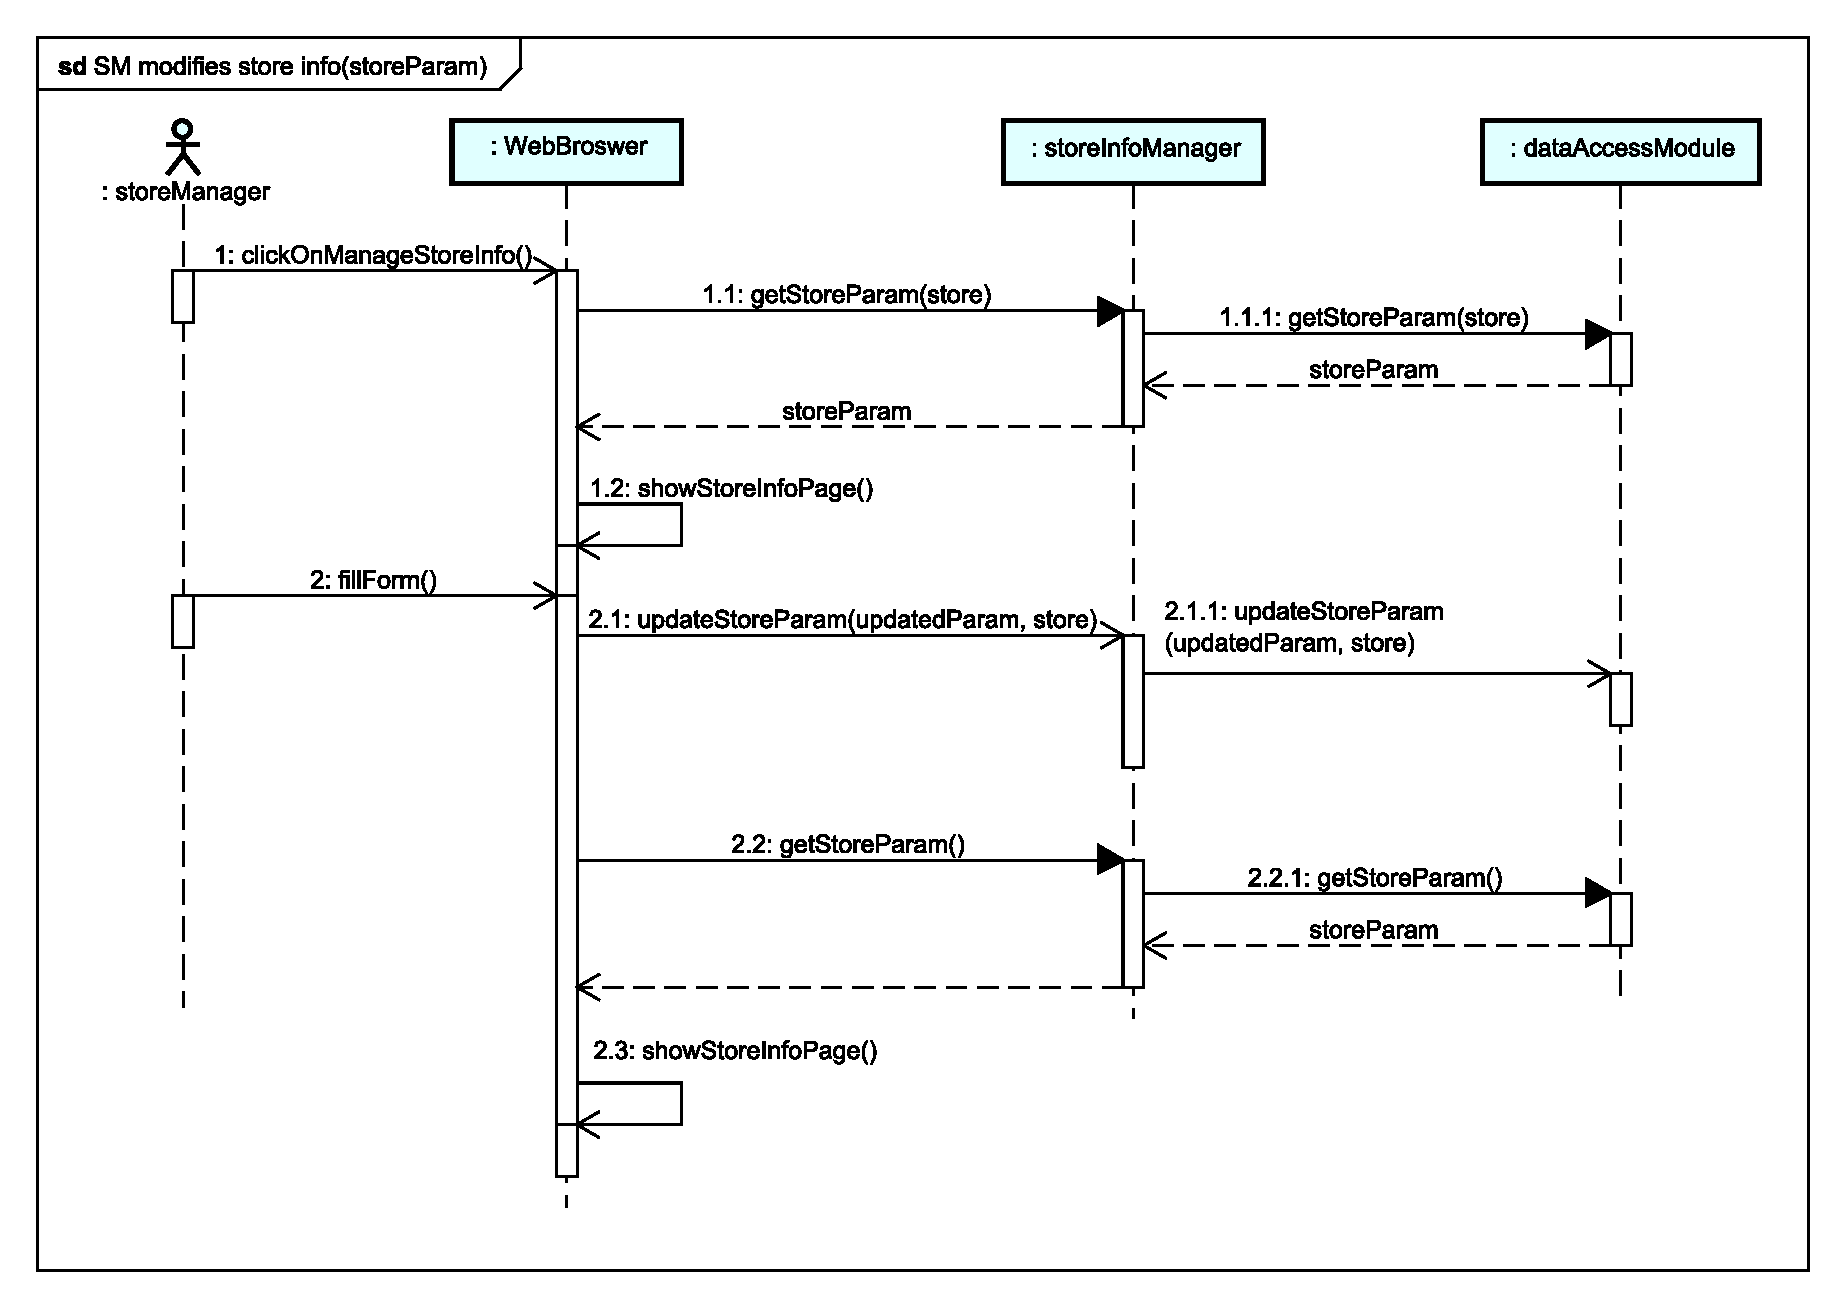
\includegraphics[width=.75\linewidth] {sequence_diagrams/SM_modifies_store_info_seqD}
	\caption{Runtime view of a Store Manager modifying their store's information}
	\label{smmodinfo} 
\end{figure}

\begin{figure}[p]	
	\centering
	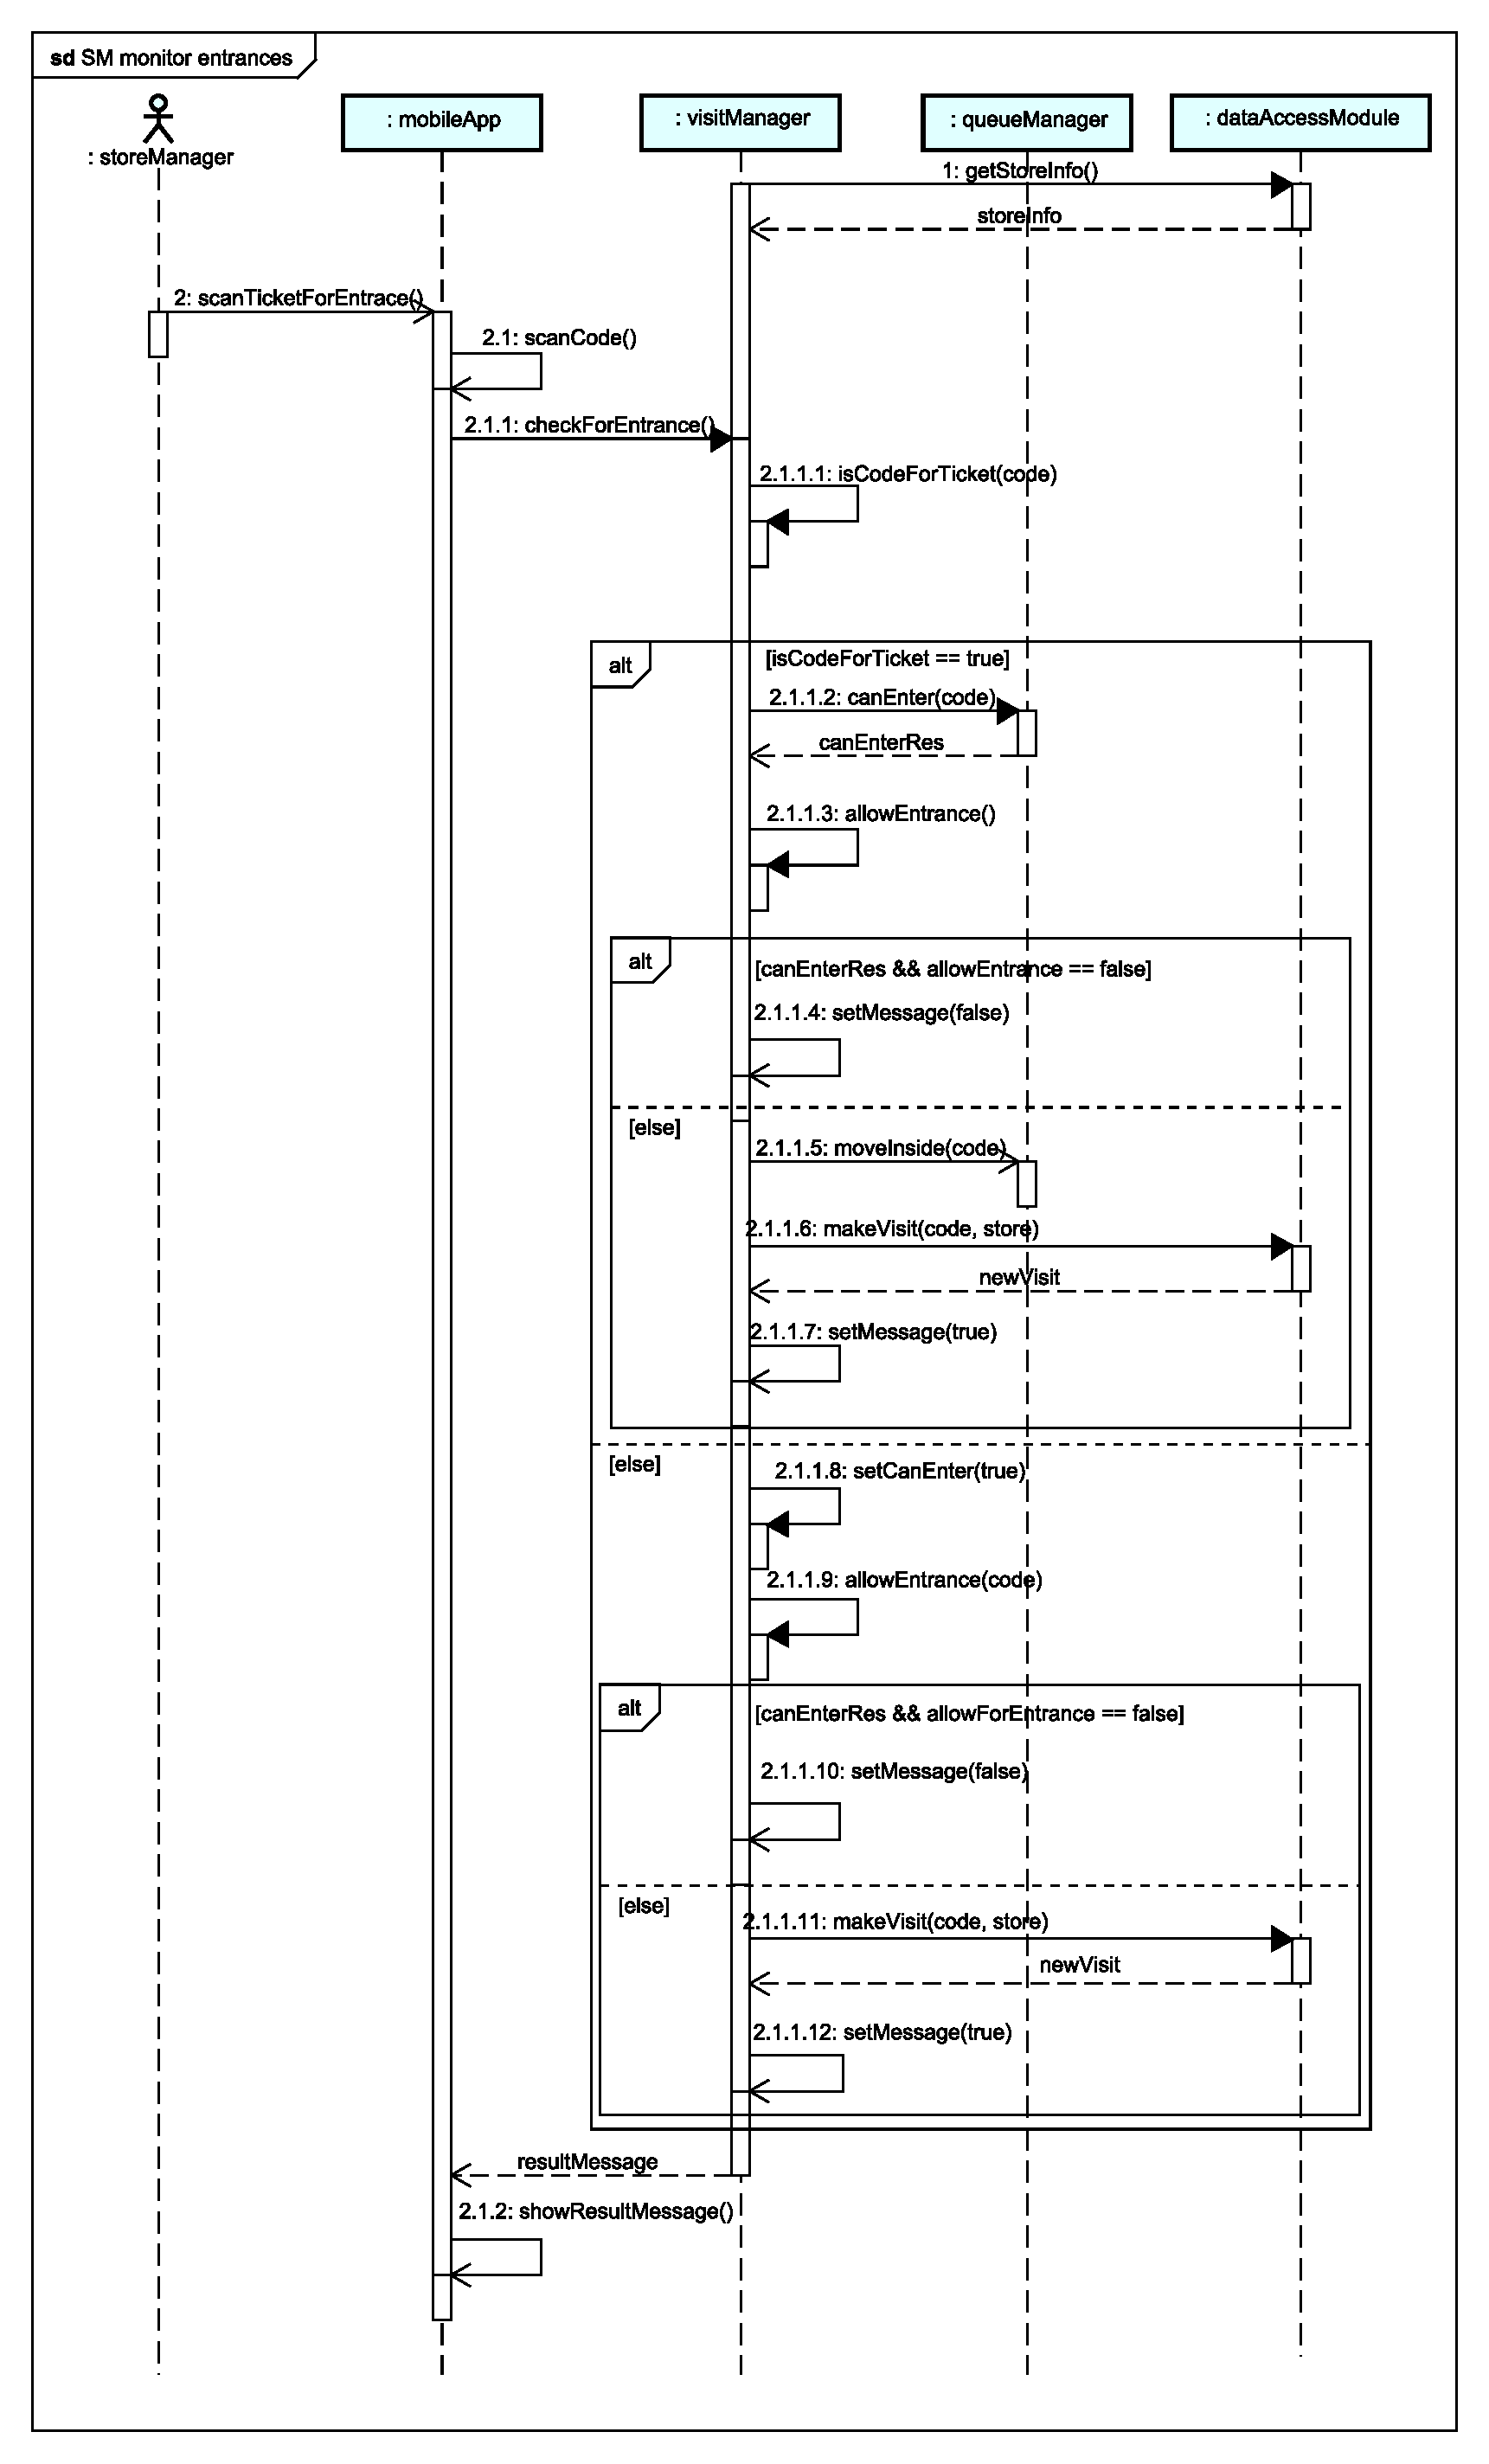
\includegraphics[height=.98\textheight] {sequence_diagrams/SM_monitor_entrances_seqD}
	\caption{Runtime view of a Store Manager monitoring accesses}
	\label{runsmmonitor} 
\end{figure}

\clearpage
% Component interfaces section, to be included in architecture.tex

\subsection{Component interfaces}
Figure \ref{intec}, Figure \ref{intsm} and Figure \ref{intstat} show the interfaces exposed by subsystems to interact with other components.

\begin{figure}[h]	
	\centering
	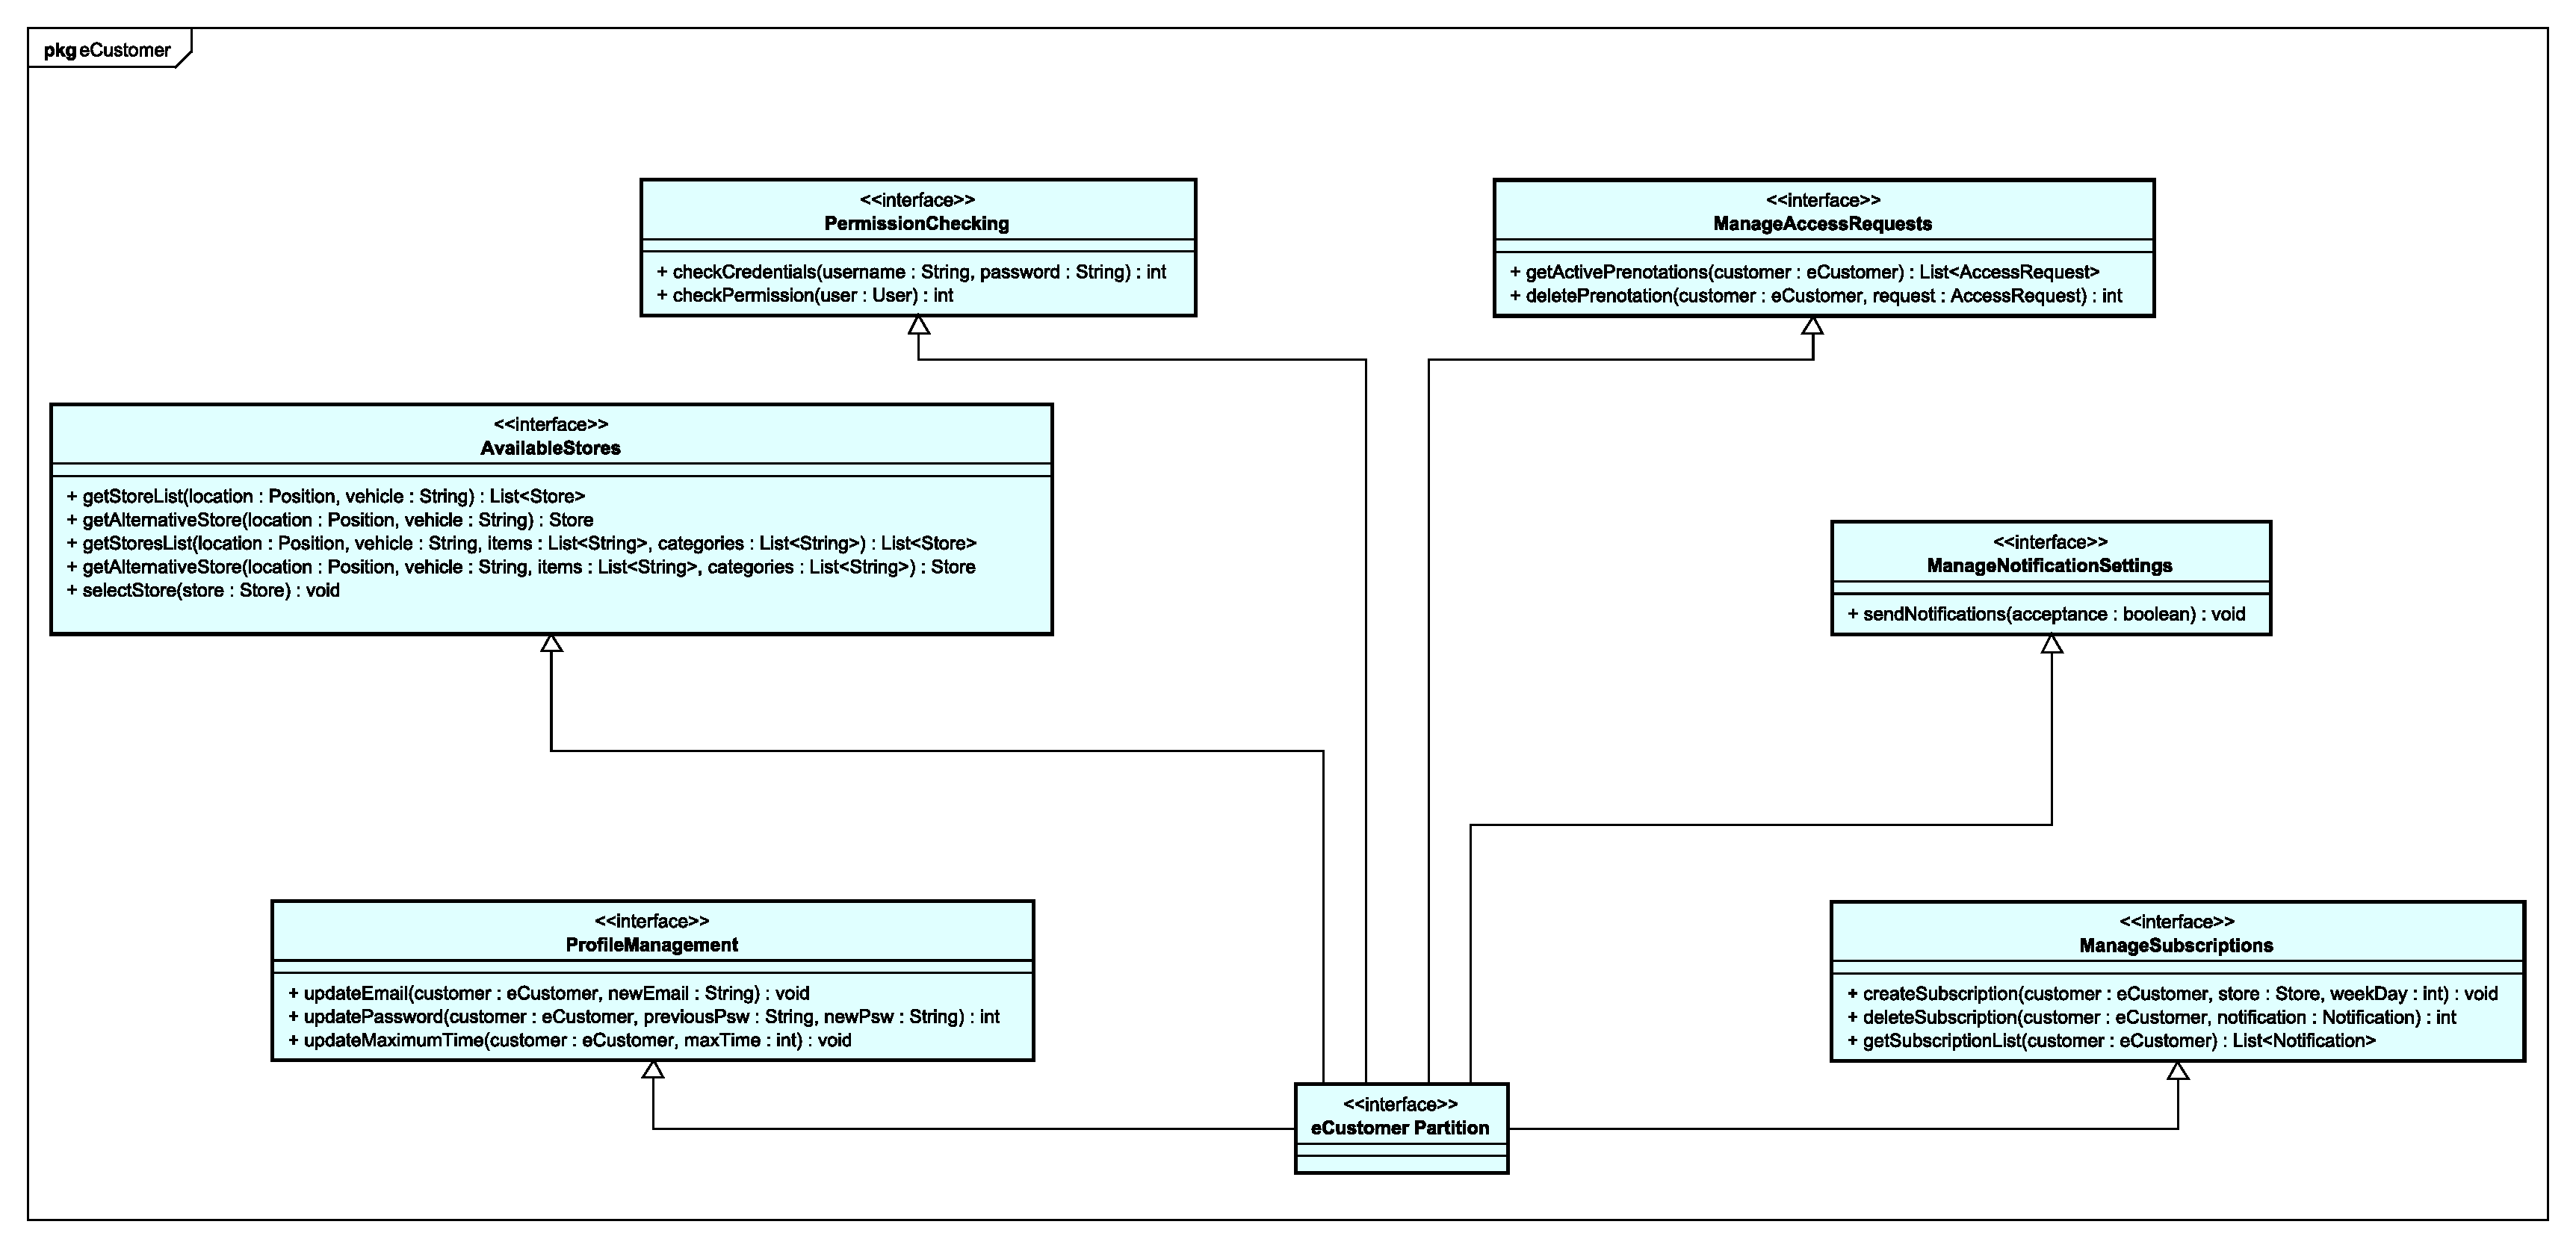
\includegraphics[width=\linewidth] {class_diagram/interface_customer}
	\caption{Component interfaces for the e-Customer subsystem}
	\label{intec}
	
	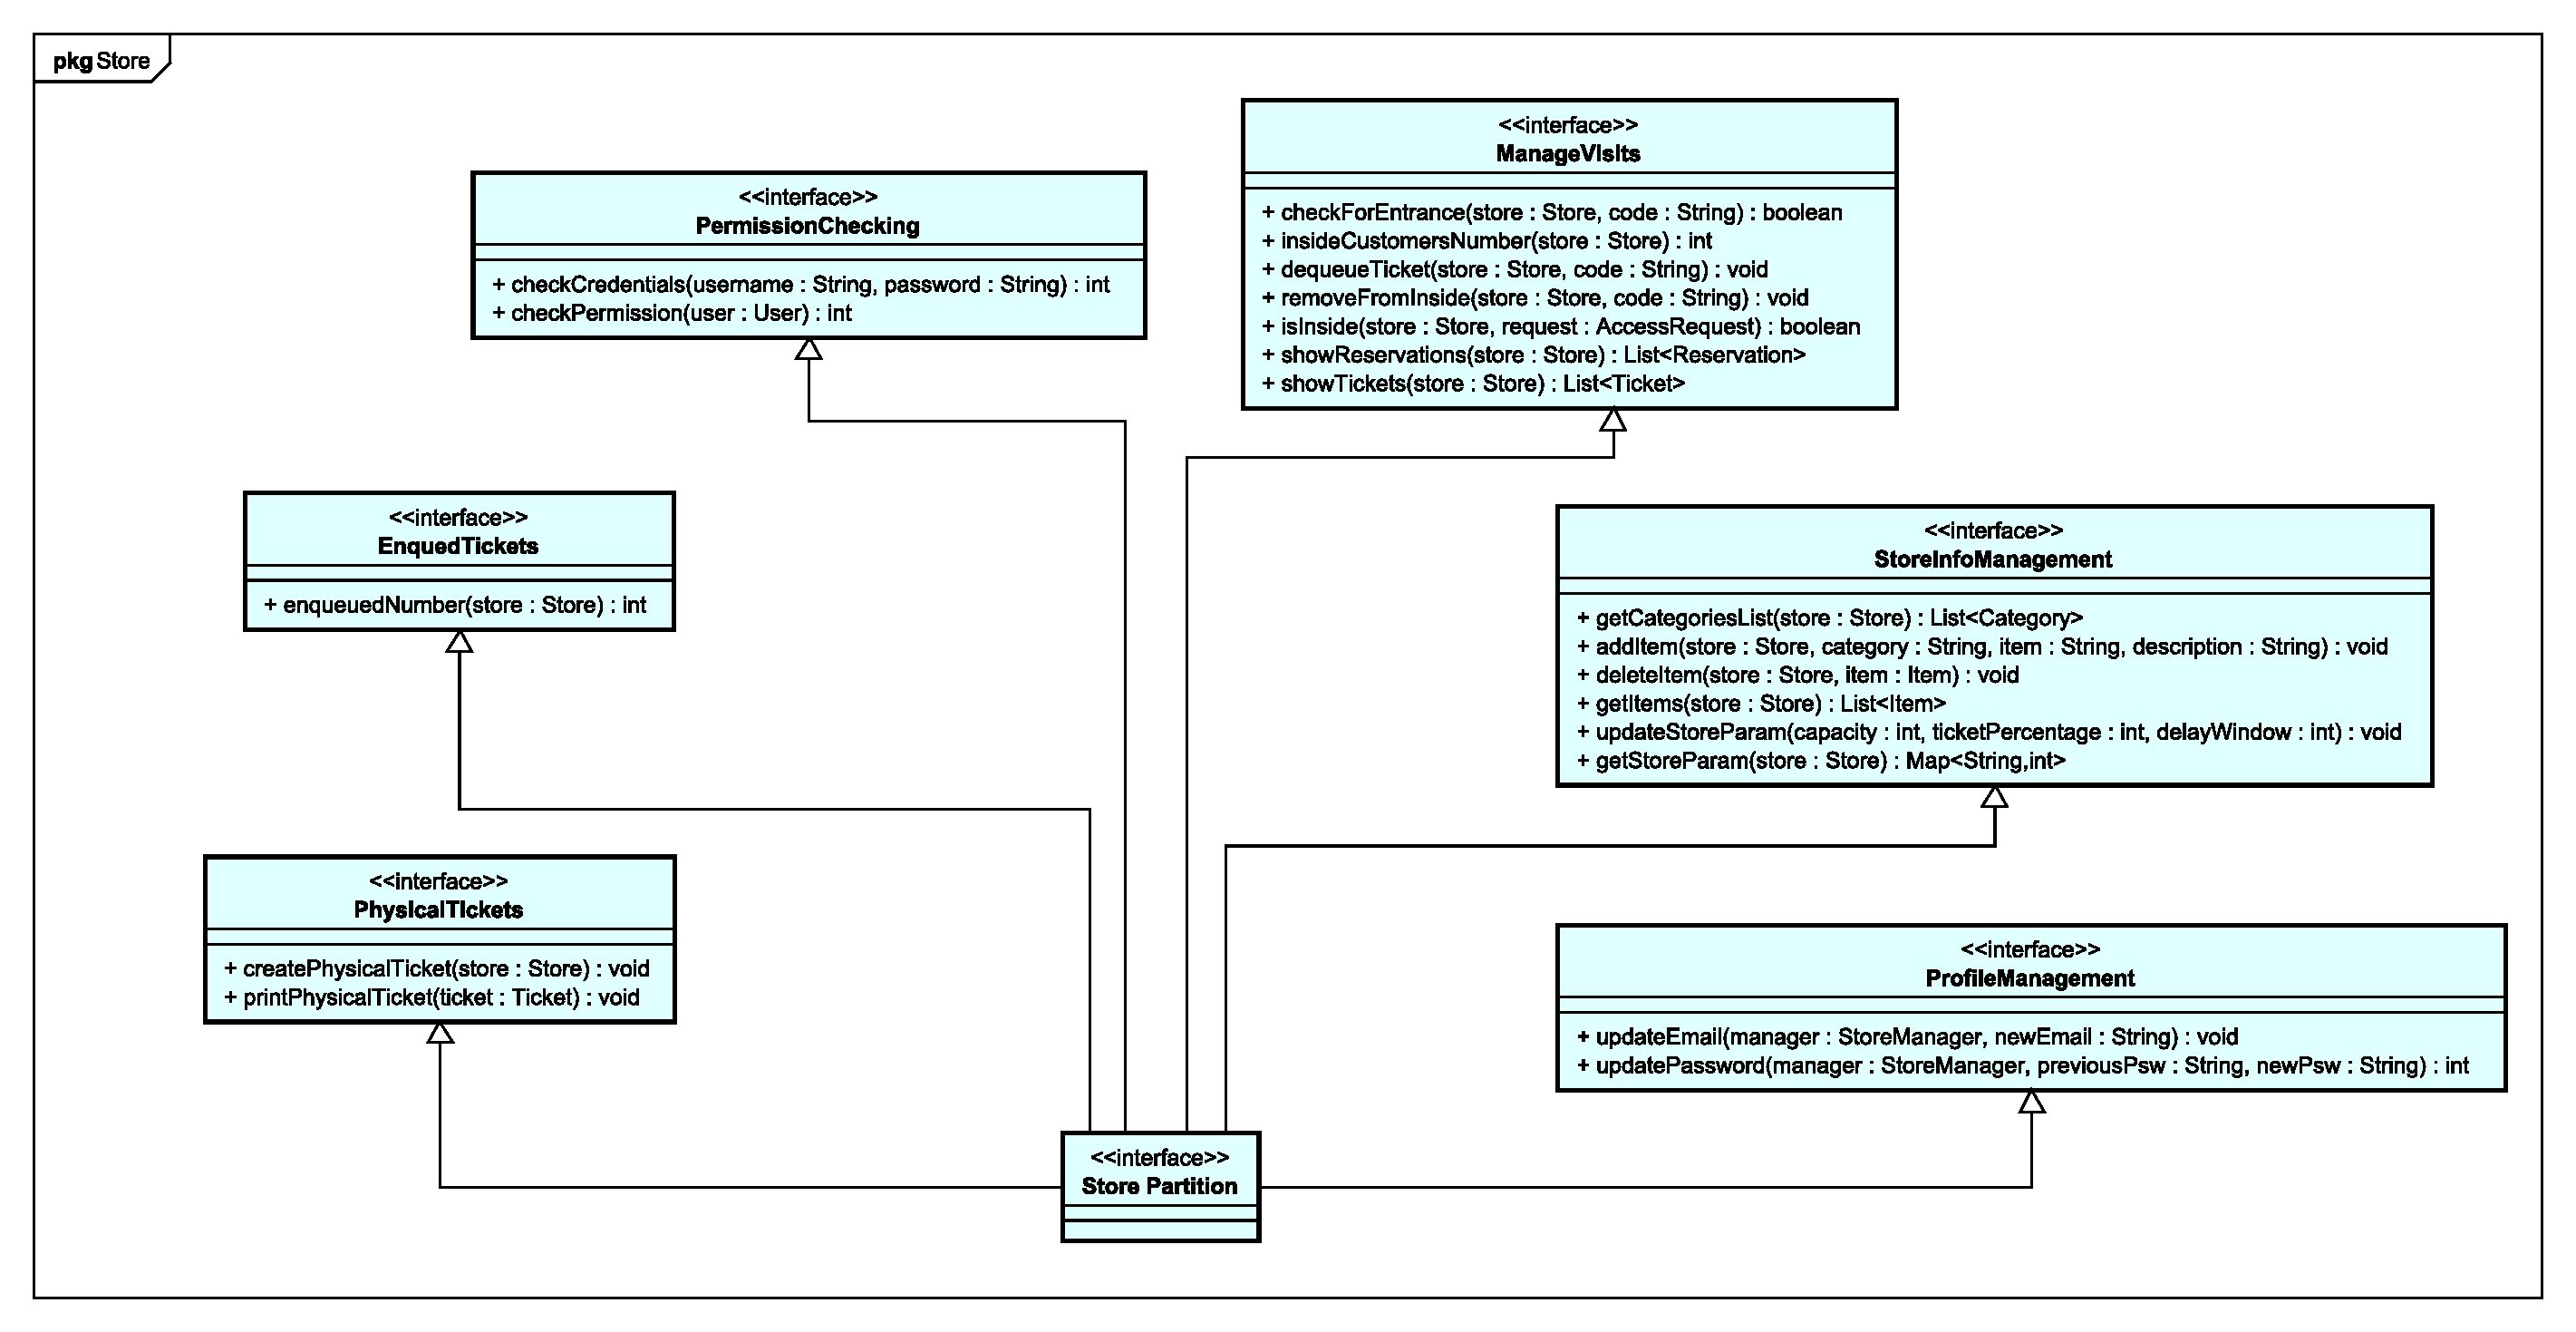
\includegraphics[width=\linewidth] {class_diagram/interface_store}
	\caption{Component interfaces for the Store Manager subsystem}
	\label{intsm}
\end{figure}

\clearpage
\begin{figure}[h]	
	\centering	
	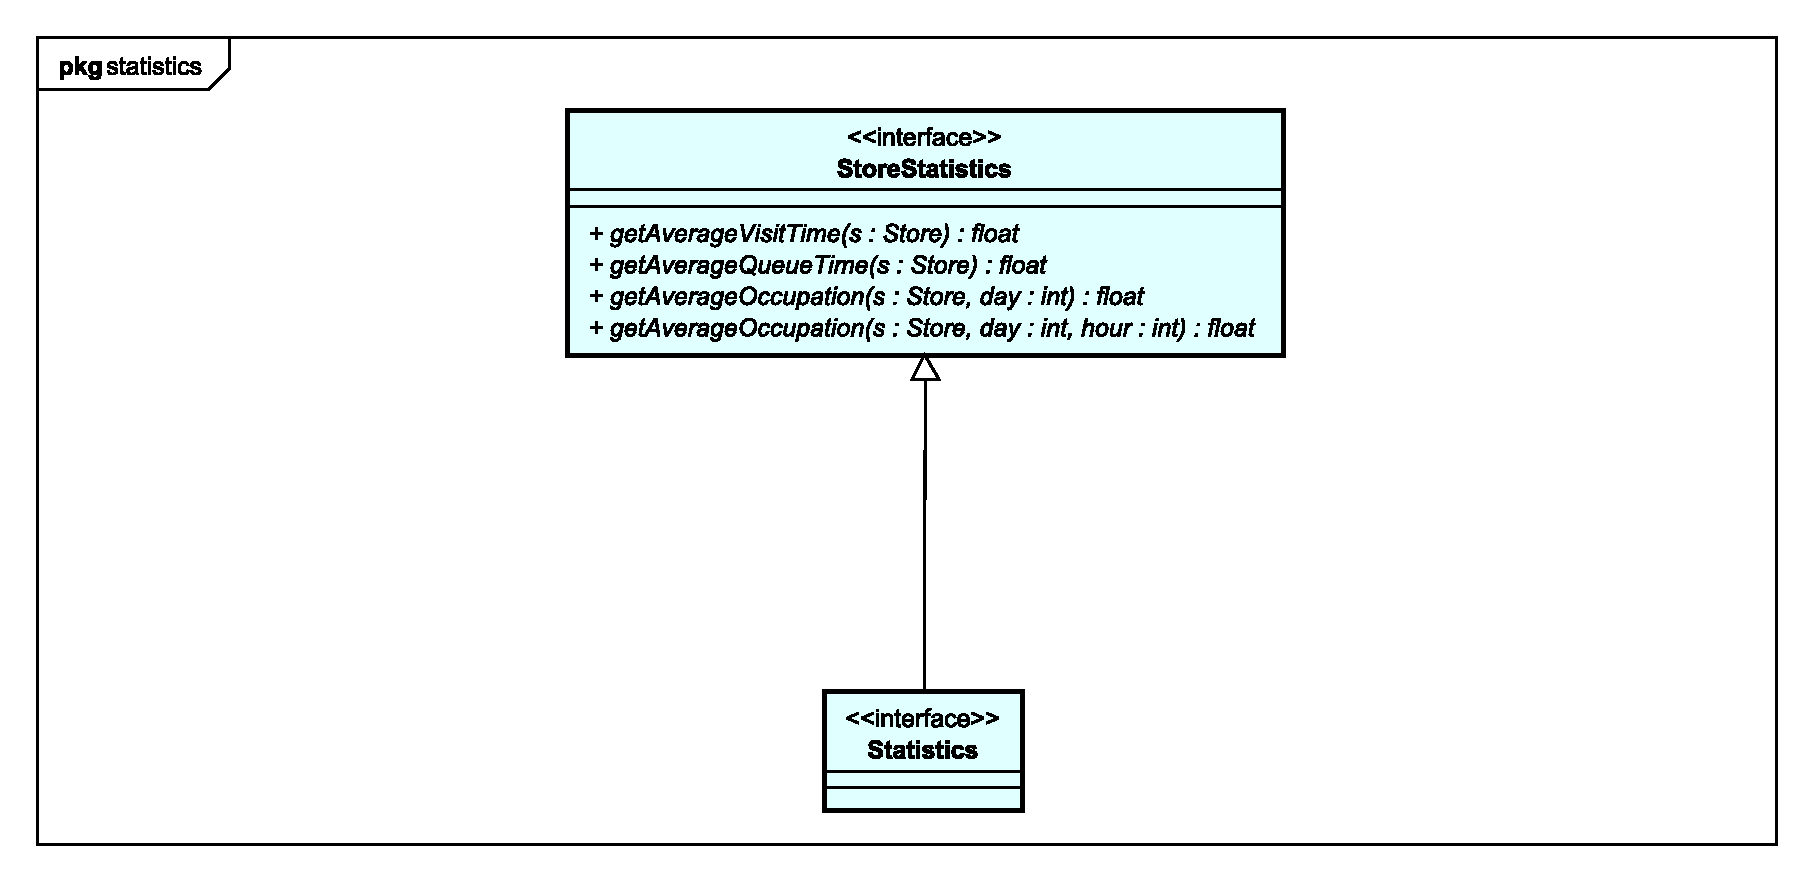
\includegraphics[width=.93\linewidth] {class_diagram/interface_statistics}
	\caption{Component interfaces for the Statistics subsystem}
	\label{intstat}
\end{figure}

\subsection{Selected architectural styles and patterns}
This section reports some directions on the use of design patterns during the implementation of the CLup system. As previously stated, the system is based on a modular design, but the following patterns are suggested:

\begin{itemize}[itemsep=-1mm, topsep=-1mm]
	\item The base architecture pattern is MVC (Model-View-Controller), as it allows to decouple the application logic from the user interaction
	\item To support MVC, the Observer Pattern\textsuperscript{\cite{observer}} should be used
	\item To have an extended interface to the database the DAO\textsuperscript{\cite{dao3}} (Data Access Object) architectural pattern is used to separate the business logic from the data tier, to moreover improve testing simplicity, to increase code readability and to make the independent from the data access technology   
	\item The application's and the online mapping system is done through an Adapter, in order to create a layer between the application and the API, and have a unified interface\textsuperscript{\cite{adapter}} for all the system's components.
	\item For what concerns the Statistic Module, a façade pattern\textsuperscript{\cite{facade}} is used to offer a unique and easy-to-use interface to its components.
	\item The frontend should use a Command pattern\textsuperscript{\cite{command}} to hide the difference among functionalities offered from the UI from a code perspective
	\item The notification module should work as a Servant to the modules using it
\end{itemize}\vspace{.5\baselineskip} 

\subsection{Other design decisions}

% Queue jumping algorithms, to be included in architecture.tex

\subsubsection{Algorithm for queue rearrangement}
In order to maximize a store occupancy, the system adopts an algorithm to let customers jump forward if a place is freed because someone dequeued; it is shown here through pseudocode. 

What is important to note is that this behaviour is based on empty places mapped 1:1 to e-Customers through notifications (physical tickets are not allowed to shift), as shown in Figure \ref{window}: every e-Customer is allowed to jump only to one place, so that their original order can be respected (if everyone accepts). An e-Customer that rejects the jump or lets the time window expire won't be asked again (in red), while, in an extreme case like the one shown (with multiple drop during one period) a customer might be asked to jump several times.

\begin{figure}[h]	
	\centering
	\includegraphics[width=.7\linewidth] {algorithms/queue}
	\caption{Visualization of the queue algorithm}
	\label{window}
\end{figure}

\paragraph{Variables}
This pseudocode assumes the existence of a queue of tickets, treated for simplicity as an array.

\paragraph{Notifier}
Every 5 minutes, a number of customers at most equal to the number of empty places is notified of an available jump, for which they won't be notified again (to avoid both multiple notifications and being notified either after a rejection or an expiration of the given time). The empty places notification order reflects the current e-Customer order.  

\begin{lstlisting}
doNotNotify = []
while(true)	
	holes = queue.getHoles()
	nextPlace = -1
	foreach(h in holes)
		nextPlace = max(nextPlace + 1, h + 1)
		while(nextplace in holes 
			or queue[nextplace] in doNotNotify)
			nextplace++
		queue[nextplace].getCustomer().notifyJumpTo(h)
		doNotNotify.add(queue[nextplace], h)
	sleep(300)
\end{lstlisting}

\paragraph{Jump}
If a customer accepts the jump, their place in queue is updated:
\begin{lstlisting}
moveTo(ticket, jumpDest)
\end{lstlisting}
% Algorithm used to generate a QR code, to be included in architecture.tex

\subsubsection{QR code generator}
This section shows how QR codes can be generated in order to ensure security and meet other design decisions of the applications. The format of the string changes based on the type of the access request, but the suggested general form consists of
\begin{center}
	\texttt{control\_character + MD5(emissionDT + storeID + accessParam)}
\end{center}
Where the \texttt{control\_character} identifies the type of request through a number and the accessParam, exclusive to the type: 
\begin{itemize}[itemsep=-1mm, topsep=-1mm]
	\item Ticket:
	\begin{itemize}[itemsep=-1mm, topsep=-1mm]
		\item \texttt{control\_character}: 0
		\item \texttt{accessParam}: nOrder
	\end{itemize}
	\item Reservation:
	\begin{itemize}[itemsep=-1mm, topsep=-1mm]
		\item \texttt{control\_character}: 1
		\item \texttt{accessParam}: entranceTime 
	\end{itemize}			
\end{itemize}\vspace{.5\baselineskip}

Through the use of MD5 all codes are guaranteed to be of length 33 characters. Figure \ref{qr} shows an example of generated QR code for a ticket with parameters:
\begin{itemize}[itemsep=-1mm, topsep=-1mm]
	\item emissionDT: 2020-12-31 10:53:31 (without spaces and special characters)
	\item storeID: 154
	\item nOrder: 51
\end{itemize}\vspace{.5\baselineskip}
That corresponds to the string
\begin{center}
	\texttt{0dd8e72b69b8e4fac5c3f3bef07e09a4a}
\end{center}

\begin{figure}[h]	
	\centering
	
\includegraphics[width=.2\linewidth] {algorithms/qr-code}
	\caption{Generated QR code}
	\label{qr}
\end{figure}

 
	
	% User interface design section
	\clearpage
	% User interface design section, to be included in dd.tex

\section{User interface design}
\label{sect:ui}
This section illustrates the UX diagrams, i.e. the transitions between the user interface's pages. The application's mock-ups can be found in the RASD.

\subsection{e-Customer UX diagram}
The e-Customer application is composed of four sections reachable through tabs:
\begin{itemize}[itemsep=-1mm, topsep=-1mm]
	\item Home page: displays some instructions to better explain the application's interfaces and functions, and how to navigate through them. Moreover, it shows the active access requests (if present)
	\item Ticket creation: allows the user to line up by filling the creation form and then choosing a store among the suggested ones
	\item Book a visit: allows the e-Customer to create a new reservation by passing through the three booking form steps and then by choosing the store they like from the list of the ones meeting the specified parameters
	\item Settings: allows e-Customers to manage notifications, subscriptions and their profile
\end{itemize}\vspace{.5\baselineskip}

These sections can be reached after the login or signup process Figure \ref{uxec} shows the transitions.

\begin{figure}[h]	
	\centering
	\includegraphics[width=\linewidth] {ux_diagrams/eCustomer_UX}
	\caption{UX diagram of the e-Customer application}
	\label{uxec} 
\end{figure}

\newpage
\subsection{Store Manager UX diagram}
The Store Manager application is composed of four sections as well:
\begin{itemize}[itemsep=-1mm, topsep=-1mm]
	\item Home page: displays instructions about the application's functionalities and gives the possibility to access other functions such as viewing store statistics or modifying the store's parameters
	\item Ticket creation: allows the Store Manager to see the enqueued tickets and to create and print physical ones
	\item Reservations: allows the Store Manager to visualize active reservations by date
	\item Settings: allows Store Manager to change information related to their profile
\end{itemize}\vspace{.5\baselineskip}
These sections can be reached after a login or signup process ended up successfully; furthermore, every screen can activate the QR code scanning function. Figure \ref{uxsm} shows the transitions 
among the interfaces.

\begin{figure}[h]	
	\centering
	\includegraphics[width=\linewidth] {ux_diagrams/StoreUX}
	\caption{UX diagram of the Store Manager application}
	\label{uxsm} 
\end{figure}

	
	% Requirements traceability section
	\clearpage
	% Requirements traceability section

\section{Requirements traceability}
\label{sect:trace}

This section illustrates which components realize each requirement previously specified in the RASD.

\paragraph{[R0] Must allow users to provide credentials}
\begin{itemize}[itemsep=-1mm, topsep=-1mm]
	\item eC Account manager module
	\item SM Account manager module	
\end{itemize}

\paragraph{[R1] Username must be unique}
\begin{itemize}[itemsep=-1mm, topsep=-1mm]
	\item eC Account manager module
	\item SM Account manager module
\end{itemize}

\paragraph{[R2] Store id must be unique}
\begin{itemize}[itemsep=-1mm, topsep=-1mm]
	\item Store info manager module
\end{itemize}

\paragraph{[R3] Must allow store managers to add or modify their store’s information}
\begin{itemize}[itemsep=-1mm, topsep=-1mm]
	\item Store info manager module
\end{itemize}

\paragraph{[R4] Users must be able to login}
\begin{itemize}[itemsep=-1mm, topsep=-1mm]
	\item eC Account manager module
	\item SM Account manager module
\end{itemize}

\paragraph{[R5] Must be able to provide the list of available stores in the user’s proximity}
\begin{itemize}[itemsep=-1mm, topsep=-1mm]
	\item Access Request module
	\item Store recommender
\end{itemize}

\paragraph{[R6] Must know the e-Customer’s position}
\begin{itemize}[itemsep=-1mm, topsep=-1mm]
	\item Access Request module
	\item Maps adapter
\end{itemize}

\paragraph{[R6.1] Must localize the e-Customer or let them provide manually a position}
\begin{itemize}[itemsep=-1mm, topsep=-1mm]
	\item Access Request module
	\item Maps adapter
\end{itemize}

\paragraph{[R7] Must assign a unique and sequential reservation id}
\begin{itemize}[itemsep=-1mm, topsep=-1mm]
	\item Access creation
\end{itemize}

\paragraph{[R8] Must generate a QR code to be scanned at entrance and exit}
\begin{itemize}[itemsep=-1mm, topsep=-1mm]
	\item Access creation
\end{itemize}

\paragraph{[R9] Must let e-Customers choose their mean of transport}
\begin{itemize}[itemsep=-1mm, topsep=-1mm]
	\item Access Request module
\end{itemize}

\paragraph{[R10] Must allow the entrance when it is the customer’s turn}
\begin{itemize}[itemsep=-1mm, topsep=-1mm]
	\item Visit manager module
	\item Queue manager module
\end{itemize}

\paragraph{[R11] Must allow a delay of at most M minutes on a customer’s turn}
\begin{itemize}[itemsep=-1mm, topsep=-1mm]
	\item Visit manager module
	\item Queue manager module
\end{itemize}

\paragraph{[R12] Must show e-Customers the number of enqueued customers in front of them}
\begin{itemize}[itemsep=-1mm, topsep=-1mm]
	\item Queue manager module
	\item Store recommender 
\end{itemize}

\paragraph{[R13] Must show users historical data on given weekdays}
\begin{itemize}[itemsep=-1mm, topsep=-1mm]
	\item Access Request module
	\item Customer visit statistics module
\end{itemize}

\paragraph{[R14] At least P\% places must be reserved for tickets}
\begin{itemize}[itemsep=-1mm, topsep=-1mm]
	\item Access Request module
	\item Store info manager module
	\item Store recommender module
\end{itemize}

\paragraph{[R15] Must notify e-Customers within a suitable time from entrance}
\begin{itemize}[itemsep=-1mm, topsep=-1mm]
	\item Customer visit statistics module
	\item Notification module 
\end{itemize}

\paragraph{[R15.1] Notification time must be based on current store occupation}
\begin{itemize}[itemsep=-1mm, topsep=-1mm]
	\item Access creation module
	\item Customer visit statistics module
	\item Notification module
\end{itemize}

\paragraph{[R15.2] Notification time must be based on estimated travel time}
\begin{itemize}[itemsep=-1mm, topsep=-1mm]
	\item Maps Adapter module
	\item Notification module
\end{itemize}

\paragraph{[R16] Must let e-Customers advance if a preceding customer dequeued}
\begin{itemize}[itemsep=-1mm, topsep=-1mm]
	\item Queue manager module
	\item Notification module
\end{itemize}

\paragraph{[R17] Must keep track of people inside the stores}
\begin{itemize}[itemsep=-1mm, topsep=-1mm]
	\item Visit manager module
\end{itemize}

\paragraph{[R17.1] Must allow scanning QR codes on entrance and exit}
\begin{itemize}[itemsep=-1mm, topsep=-1mm]
	\item Visit manager module
\end{itemize}

\paragraph{[R18] Must not allow the entrance of more customers than prescribed}
\begin{itemize}[itemsep=-1mm, topsep=-1mm]
	\item Visit manager module
\end{itemize}

\paragraph{[R20] Physical tickets must be placed on the same queue as virtual ones}
\begin{itemize}[itemsep=-1mm, topsep=-1mm]
	\item Access creation module
	\item Queue manager module
\end{itemize}

\paragraph{[R21] Physical tickets must be printed}
\begin{itemize}[itemsep=-1mm, topsep=-1mm]
	\item Access Creation module
\end{itemize}

\paragraph{[R22] Must allow Physical Customers to scan their code in order to dequeue}
\begin{itemize}[itemsep=-1mm, topsep=-1mm]
	\item Visit manager module
\end{itemize}

\paragraph{[R23] e-Customers who book a visit must be allowed to enter at their chosen time}
\begin{itemize}[itemsep=-1mm, topsep=-1mm]
	\item Visit manager module
\end{itemize}

\paragraph{[R24] Must let e-Customers insert the expected duration of the visit}
\begin{itemize}[itemsep=-1mm, topsep=-1mm]
	\item Access Request module
\end{itemize}

\paragraph{[R24.1] Must be able to infer and suggest the duration for long term customers}
\begin{itemize}[itemsep=-1mm, topsep=-1mm]
	\item Customer visit statistics module
\end{itemize}

\paragraph{[R25] Must let e-Customers insert a list of items/categories they intend to buy}
\begin{itemize}[itemsep=-1mm, topsep=-1mm]
	\item Access Request module
\end{itemize}

\paragraph{[R26] Alternatives must be based on information provided by the e-Customer and store occupation (both real time and historical)}
\begin{itemize}[itemsep=-1mm, topsep=-1mm]
	\item Requests manager module
	\item Queue manager module
	\item Customer visit statistics module
	\item Store occupation stats module
	\item Store recommender module
	\item Maps adapter module
\end{itemize}

\paragraph{[R27] e-Customers must be able to subscribe to the notification service}
\begin{itemize}[itemsep=-1mm, topsep=-1mm]
	\item Subscription module
\end{itemize}

\paragraph{[R28] Must let e-Customers unsubscribe from the notification service}
\begin{itemize}[itemsep=-1mm, topsep=-1mm]
	\item Subscription module
\end{itemize}

\paragraph{[R29] The system must notify the e-Customers based on their choices}
\begin{itemize}[itemsep=-1mm, topsep=-1mm]
	\item Subscription module
	\item Store occupation stats module
	\item Notification module
\end{itemize}

		
	% IIT section
	\clearpage
	% Implementation, integration and test plan, to be included in dd.tex

\section{Implementation, integration and test plan}
\label{sect:iit}
This section reports the guidelines to implement and test the CLup application. The chosen approach consists in a bottom-up development based on the dependency graph identified in Figure \ref{dep}.

\subsection{Implementation}
The chosen order of implementation, based on the highlighted dependencies and aimed at obtaining core functionalities as soon as possible is the following:
\begin{itemize}[itemsep=-1mm, topsep=-1mm]
	\item Data Access Module
	\item Maps Adapter
	\item SM Account Manager Module
	\item eC Account Manager Module
	\item Queue Manager Module
	\item Visit Manager Module
	\item Access Creation Module
	\item Store Info Manager Module
	\item Store Statistics
	\item Customer Statistics
	\item Store Recommender Module
	\item Access Request Module
	\item Notification Module
	\item Requests Manager Module
	\item Subscription Module
\end{itemize}\vspace{.5\baselineskip} 

If the team is able to handle a good level of parallelization, Figure \ref{deptime} shows a suggestion of steps aimed at minimizing the overall development time; each module's length is dimensioned based on its expected implementation difficulty, and the critical path (that needs not to be delayed in order to meet potential deadlines) is highlighted in red. The graph is also useful for determining which elements can be delayed without impacting the total development time.

\begin{landscape}
	\begin{figure}[p]
		\centering	
		\includegraphics[width=\linewidth] {iit/dependency_graph}
		\caption{Dependency graph}
		\label{dep} 
	\end{figure}

	\begin{figure}[p]
		\centering	
		\includegraphics[width=\linewidth] {iit/dependency_time}
		\caption{Dependency graph with expected time and critical path highlighted}
		\label{deptime} 
	\end{figure}
\end{landscape}

\subsection{Integration and Testing}
\subsubsection{Unit testing}
The unit test can be performed as soon as a component has been developed, or even during its realization to better check its conformity to requirements. Having chosen a bottom-up approach, only Drivers are needed in order to correctly perform unit tests.

% Integration strategy section, to be included in iit.tex

\subsubsection{Integration strategy}
The implementation order has been developed considering the possibility to immediately integrate components and test their interactions; this way development time can be optimized even more and errors can be found as early as possible. The integration strategy is shown in the following figures.

\begin{figure}[h]
	\begin{subfigure}{.42\textwidth}
		\centering
		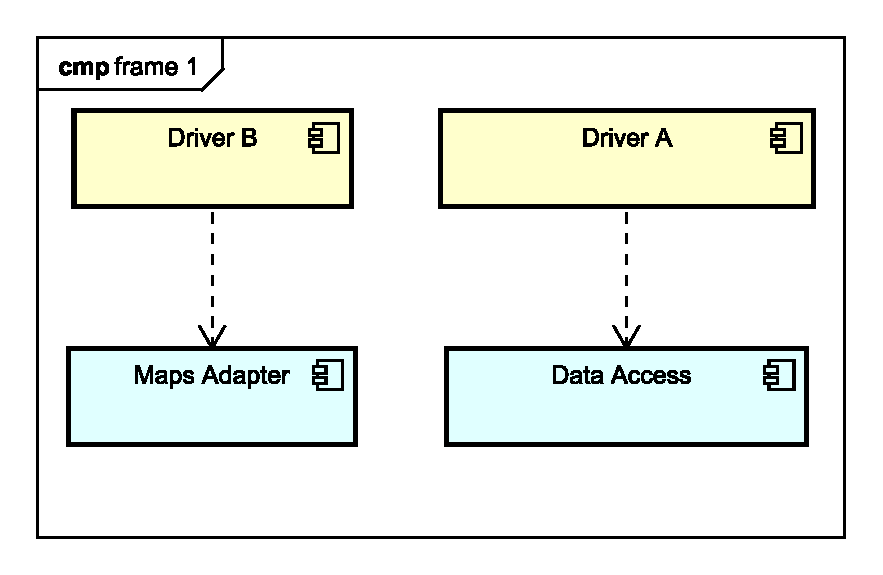
\includegraphics[width=\linewidth]{iit/frame_1}
		\caption{First components with their drivers}
		\label{frame_1}
	\end{subfigure}
	\begin{subfigure}{.58\textwidth}
		\centering
		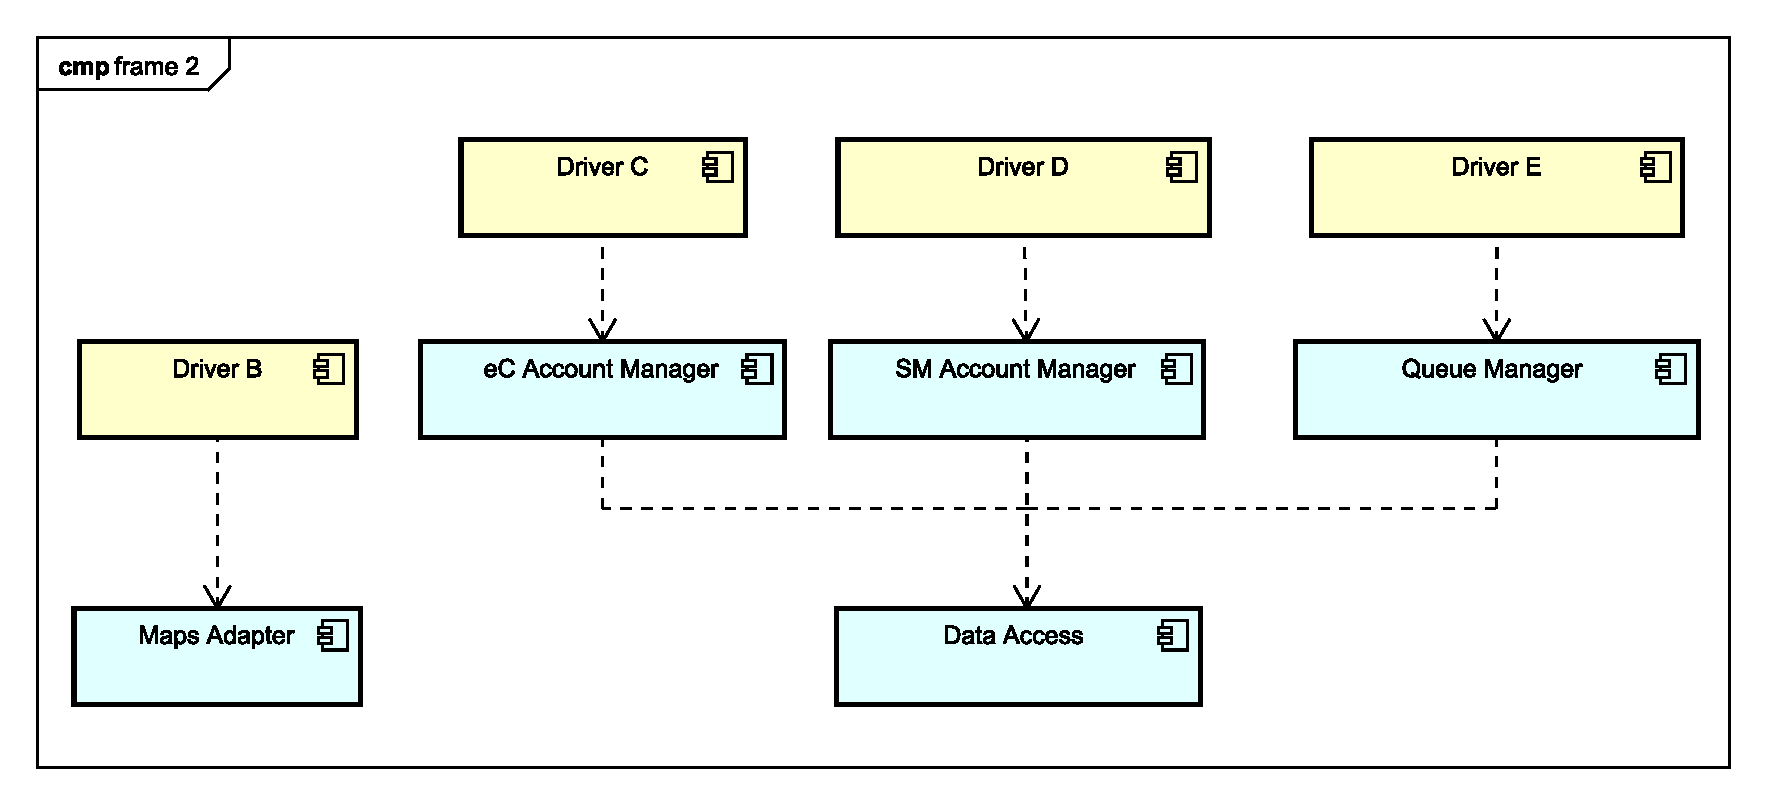
\includegraphics[width=\linewidth]{iit/frame_2}
		\caption{Adding some modules that use function provided by the Data Access and their drivers}
		\label{frame_2}
	\end{subfigure}
\end{figure}

\begin{figure}[h]
	\centering	
	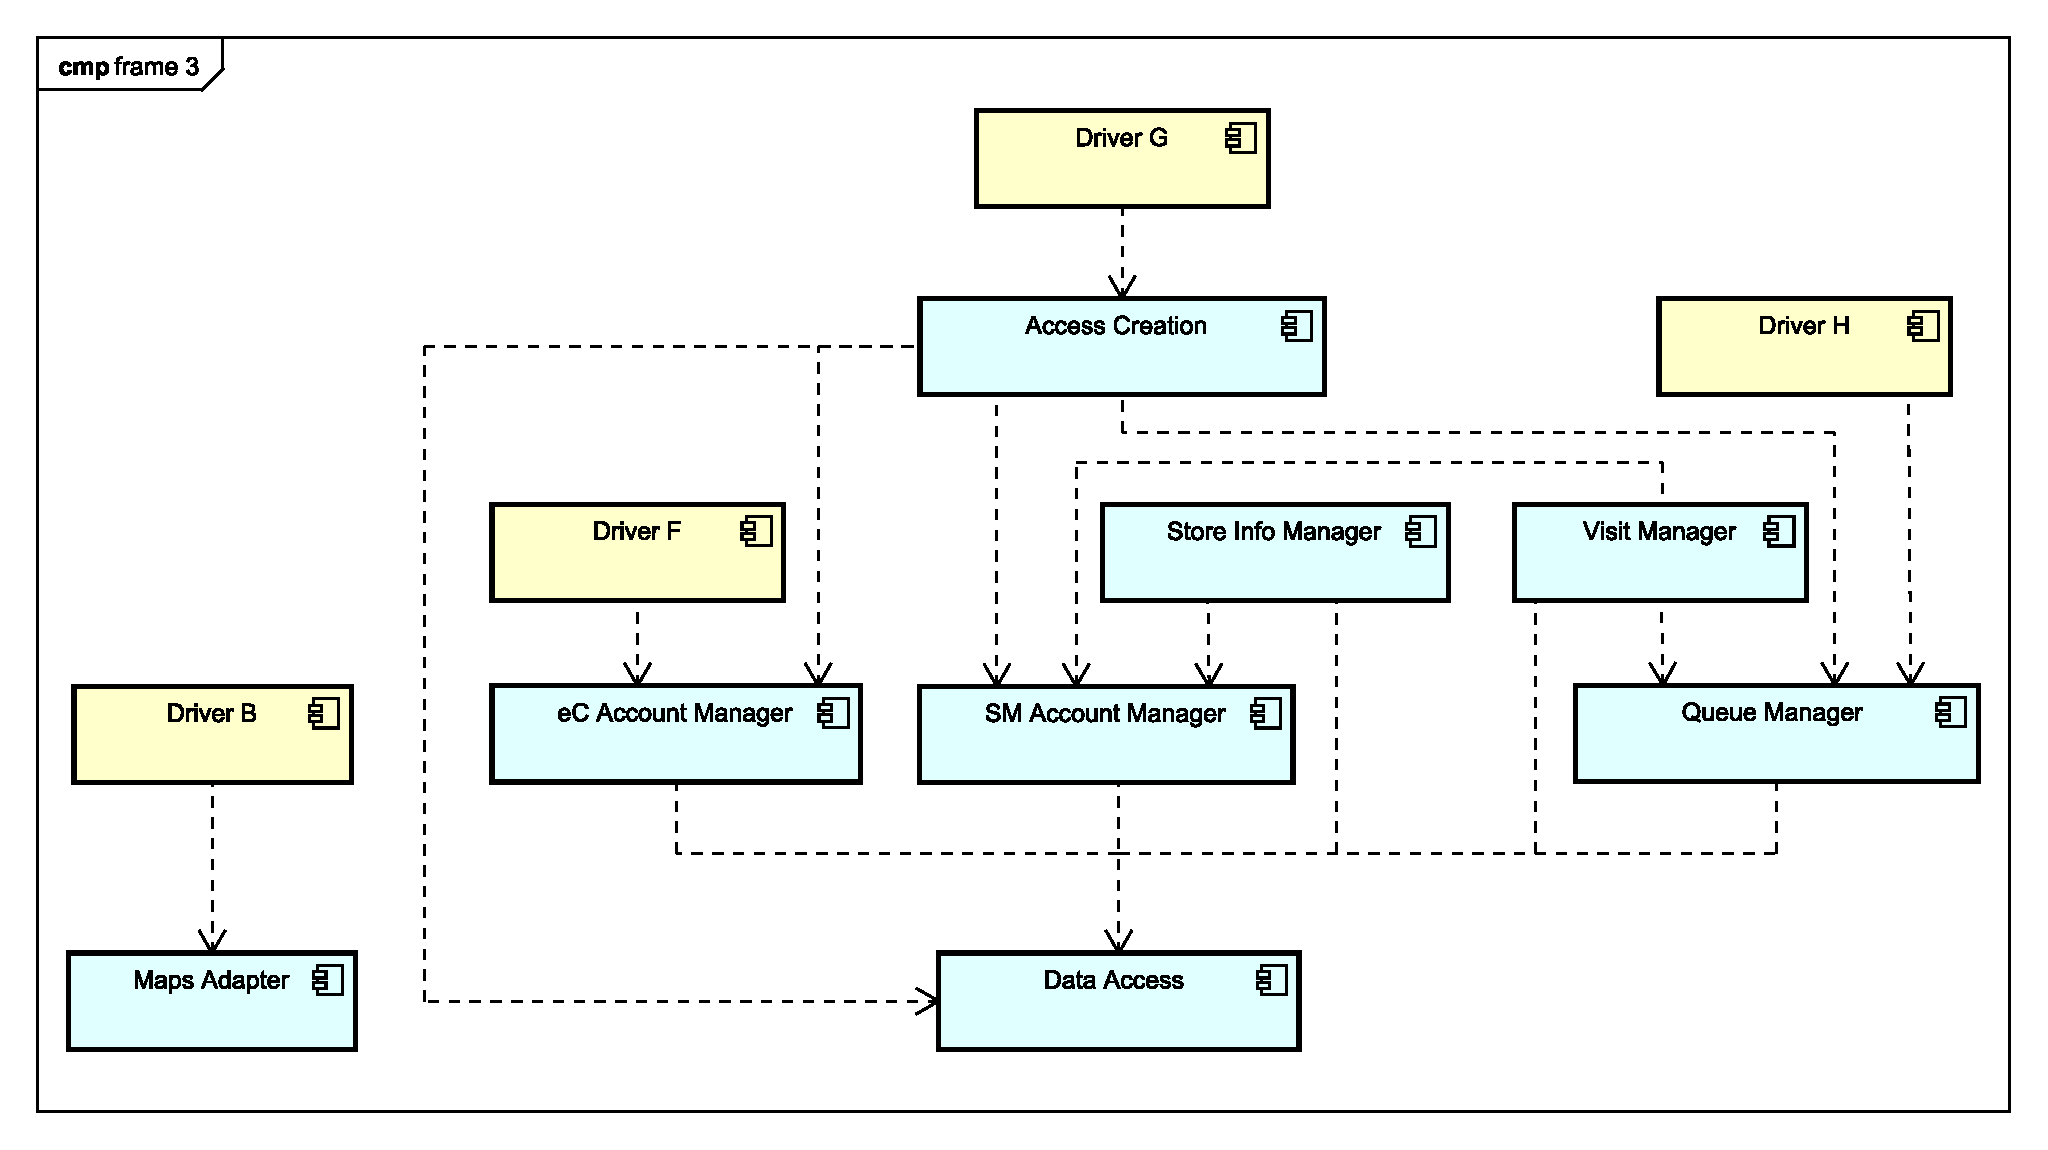
\includegraphics[width=\linewidth] {iit/frame_3}
	\caption{Realization of Access Creation, Store Info Manager, and Visit Modules}
	\label{frame_3} 
\end{figure}

\begin{figure}[p]
	\centering	
	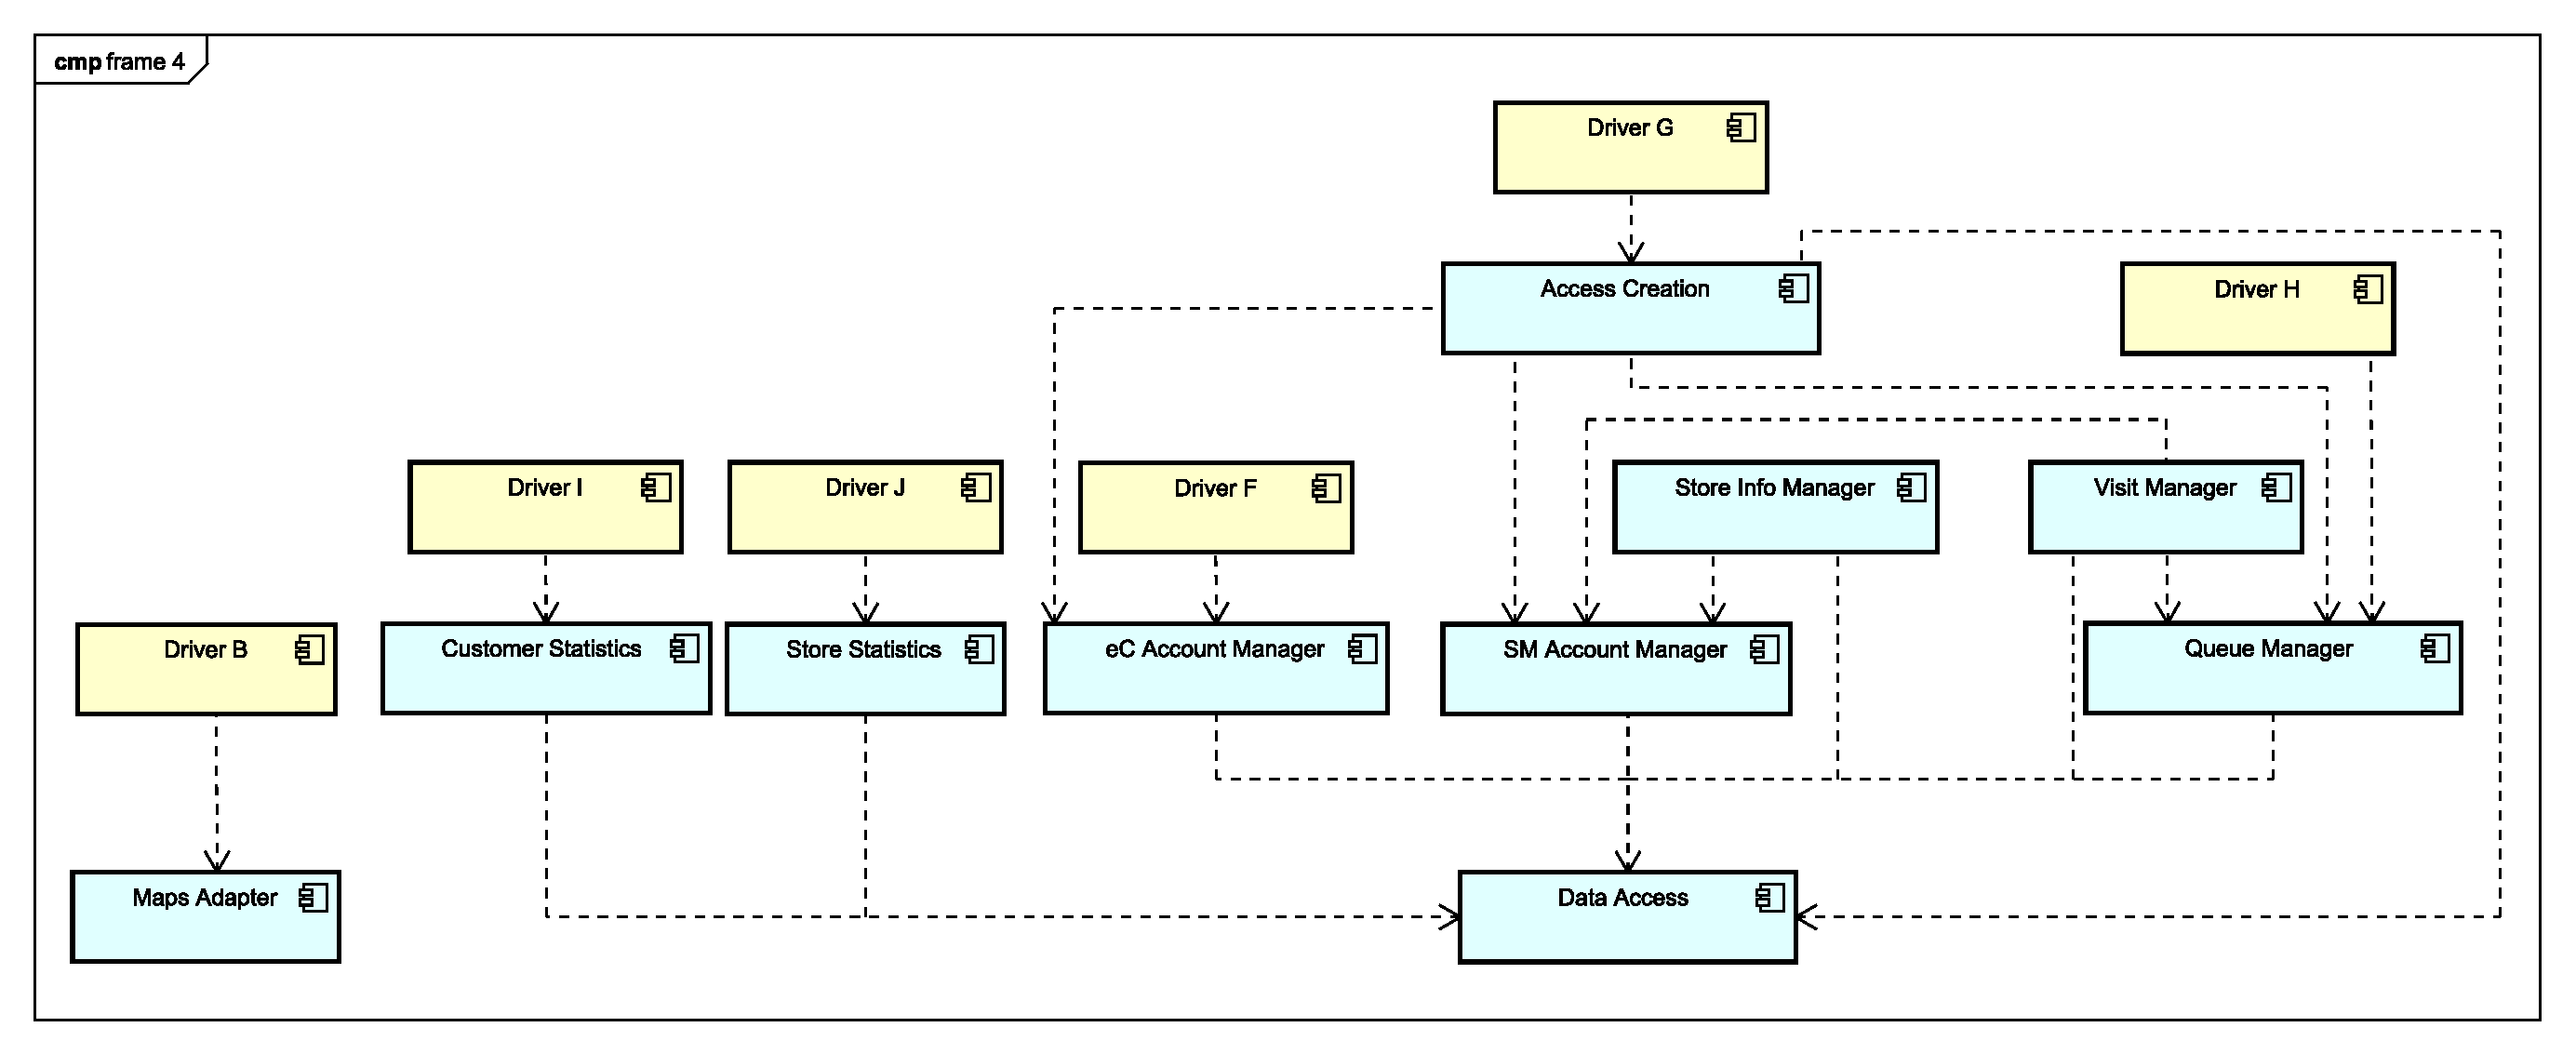
\includegraphics[width=\linewidth] {iit/frame_4}
	\caption{Implementation and integration of Statistics and Store Info Manager Modules}
	\label{frame_4} 

	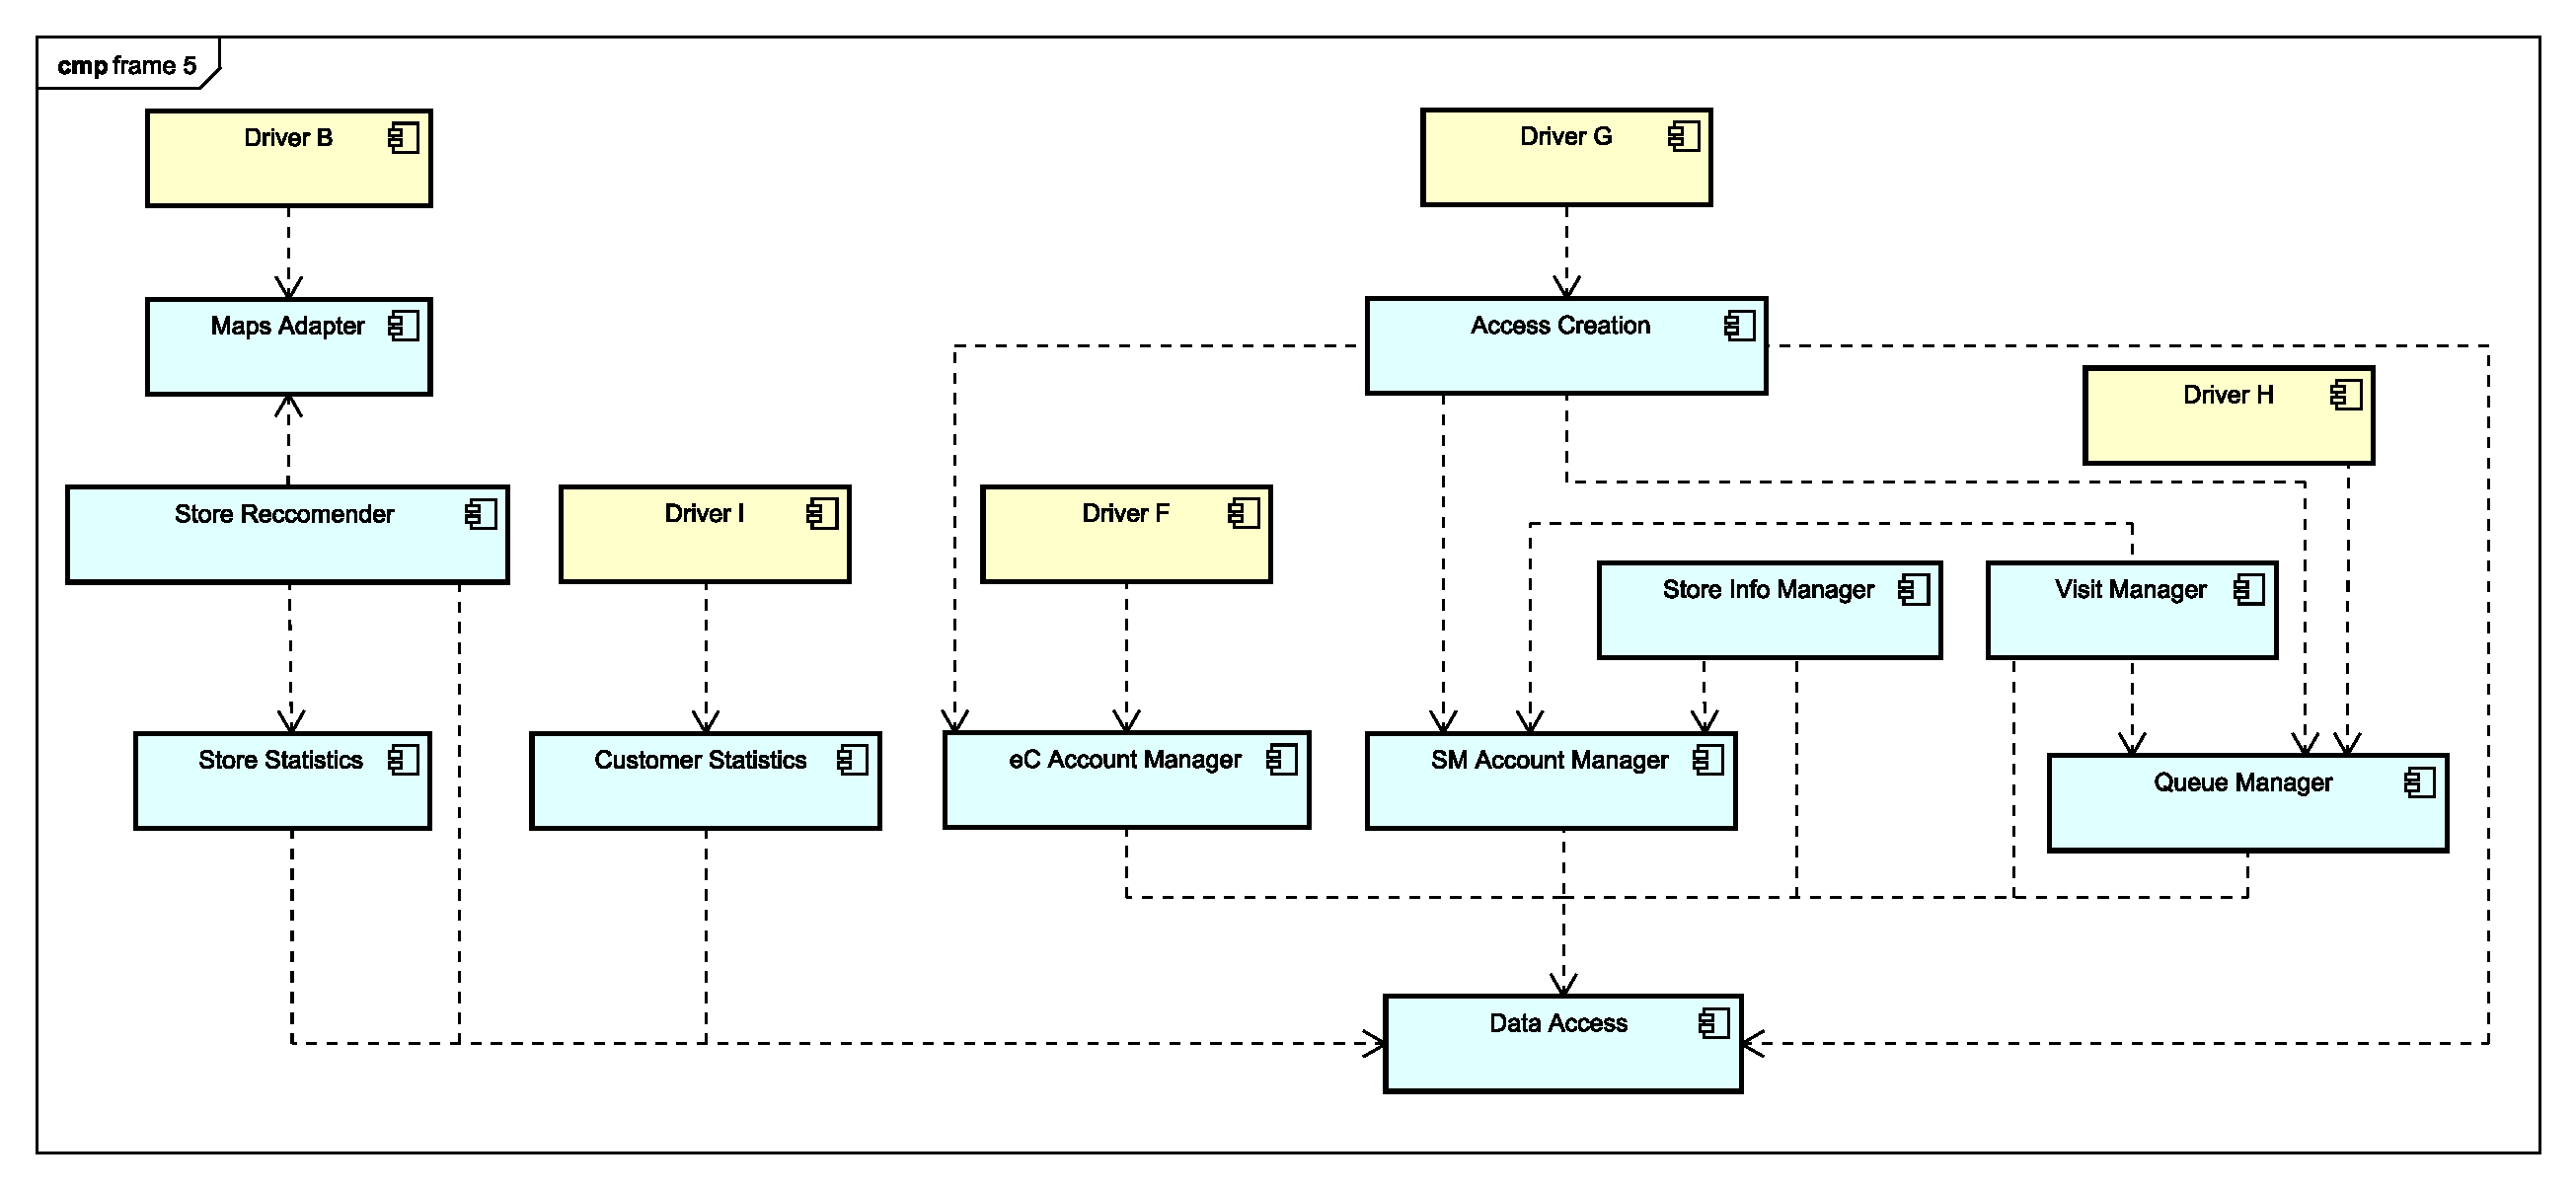
\includegraphics[width=\linewidth] {iit/frame_5}
	\caption{Adding the Store Recommender Module and integrating it with its dependencies}
	\label{frame_5} 

	\centering	
	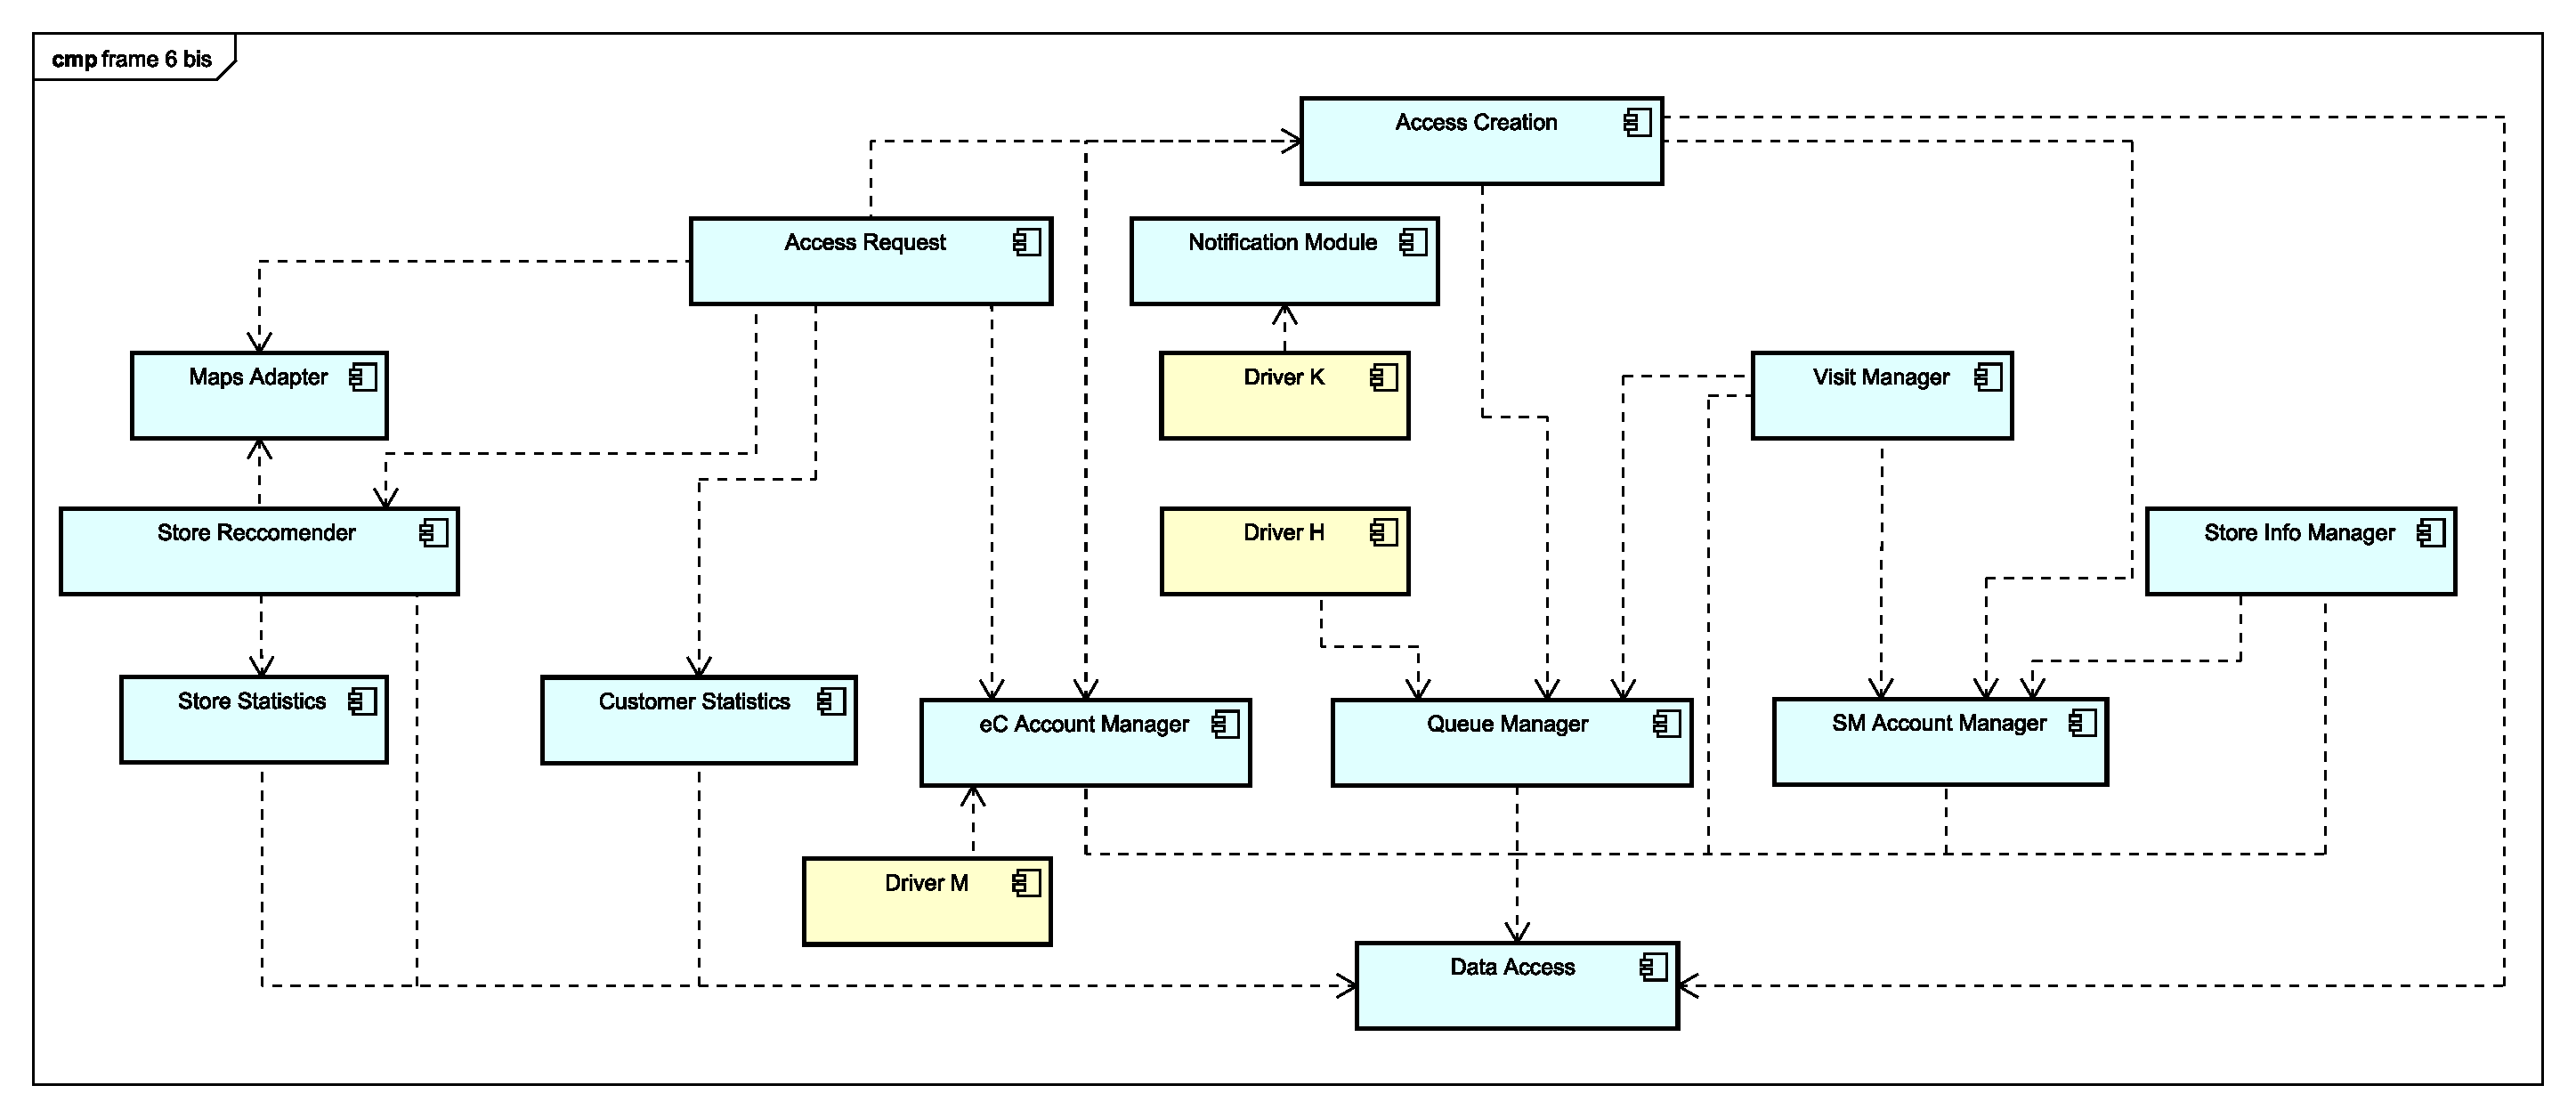
\includegraphics[width=\linewidth] {iit/frame_6}
	\caption{Integration of Access Request and Notification Modules}
	\label{frame_6} 
\end{figure}

\begin{figure}[h]
	\centering	
	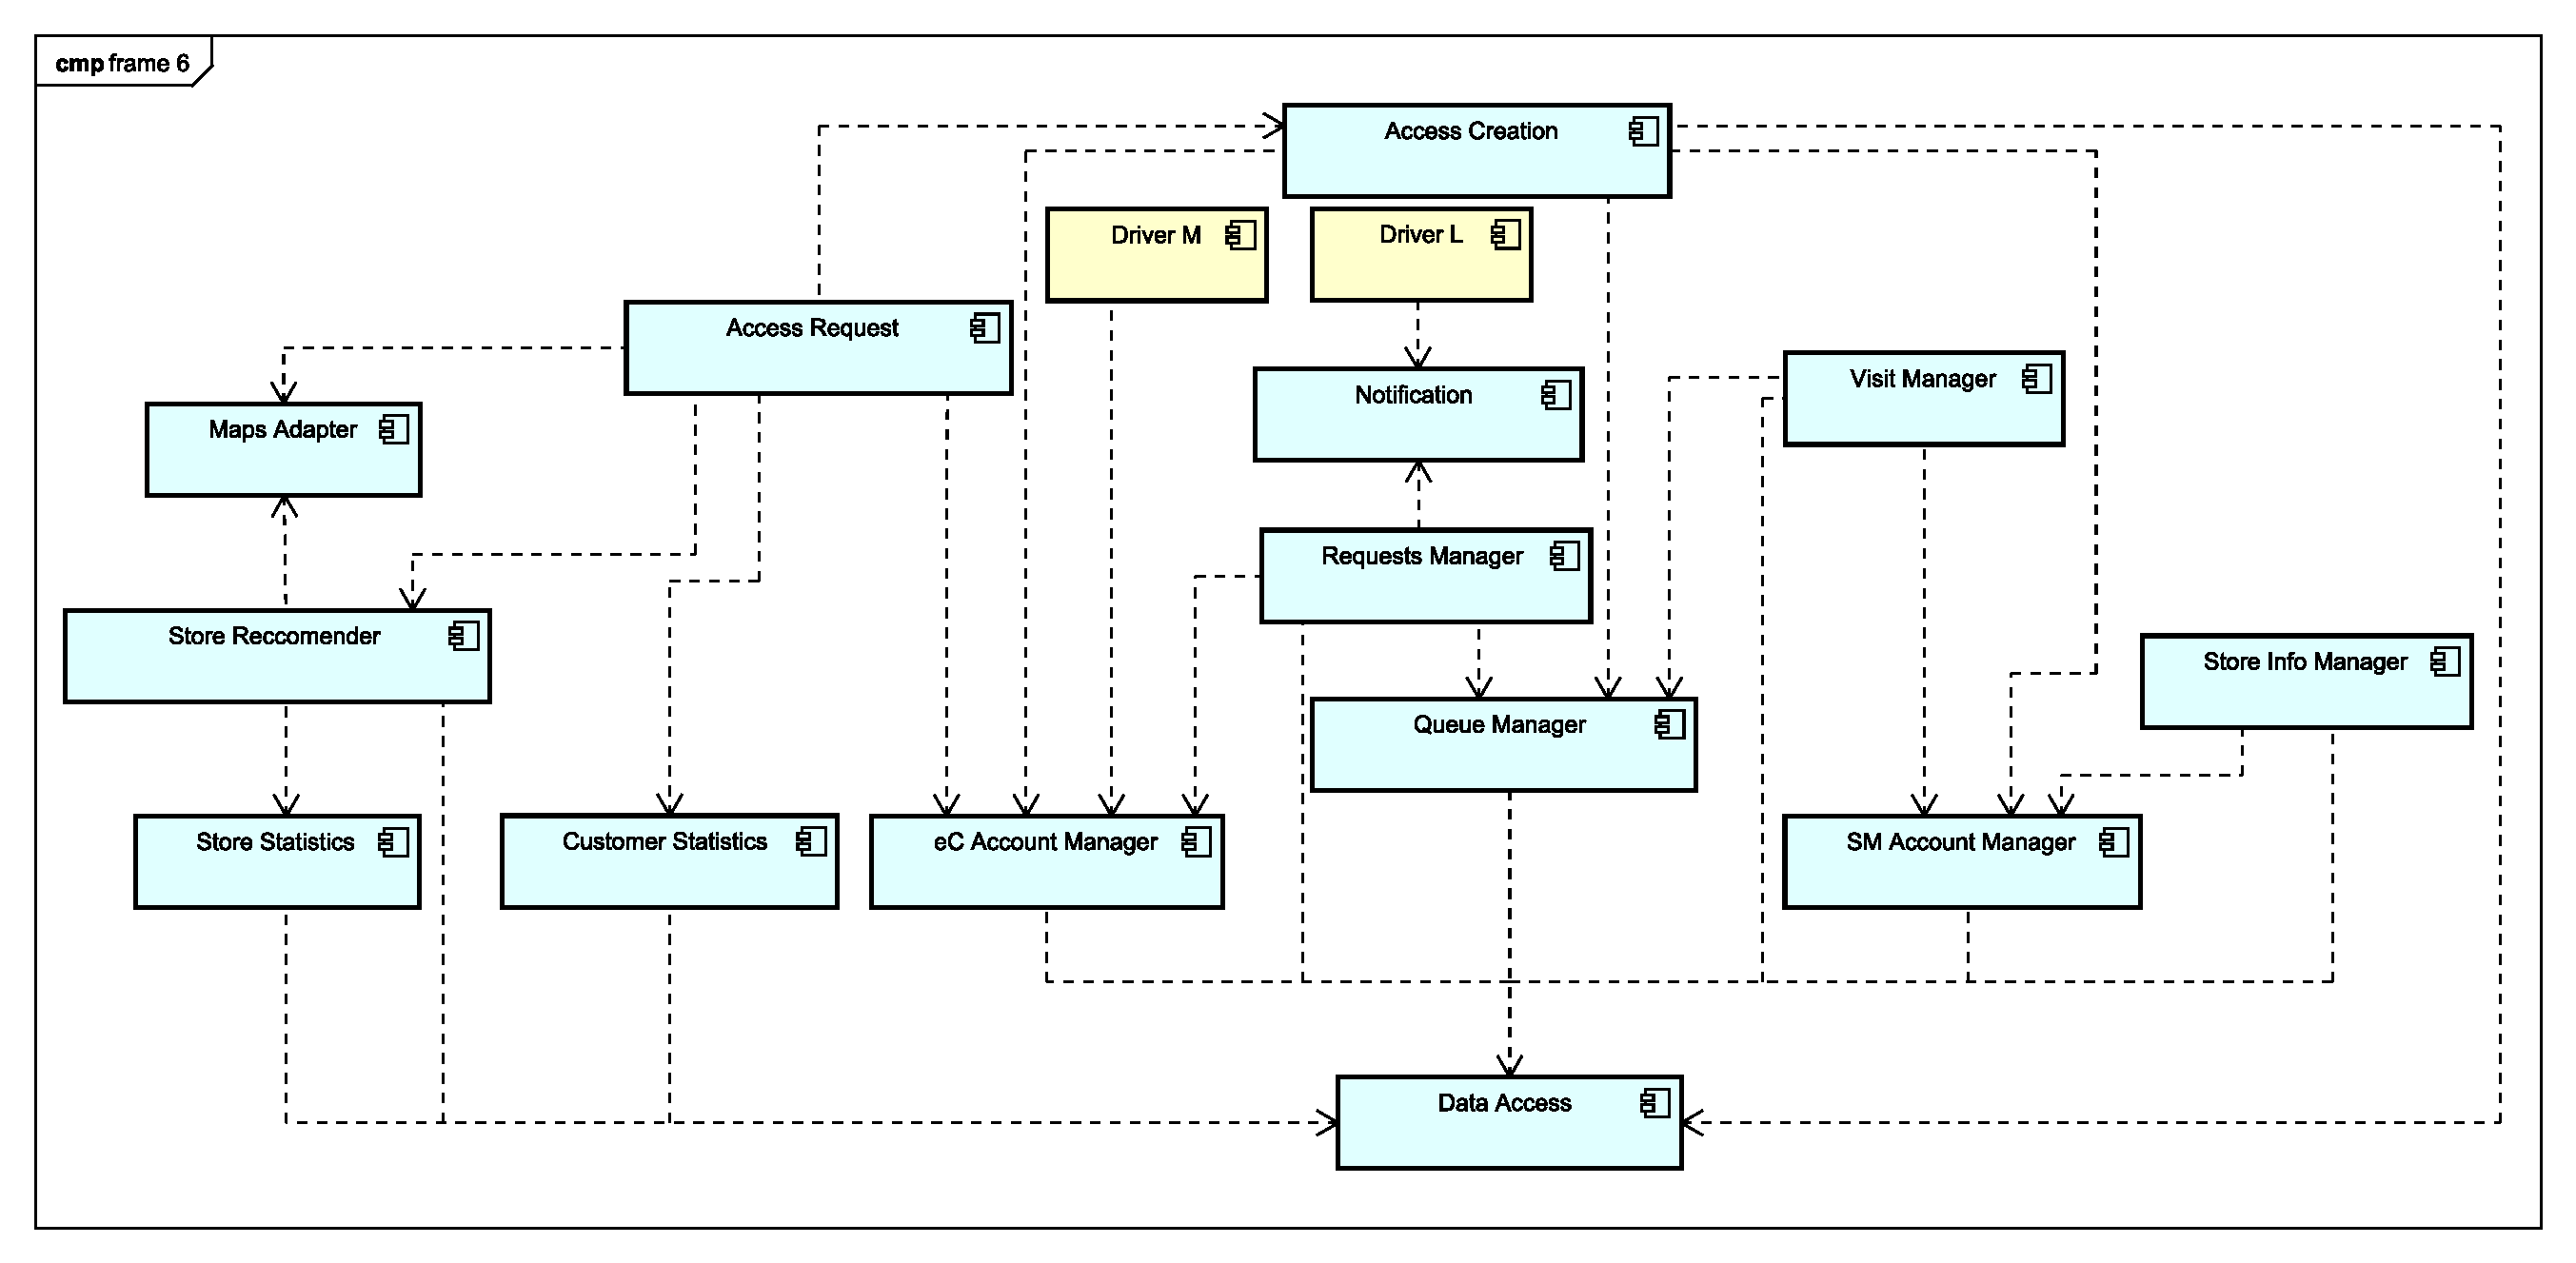
\includegraphics[width=\linewidth] {iit/frame_7}
	\caption{Addition of the Requests Manager Module}
	\label{frame_7} 
\end{figure}

\begin{figure}[h]
	\centering	
	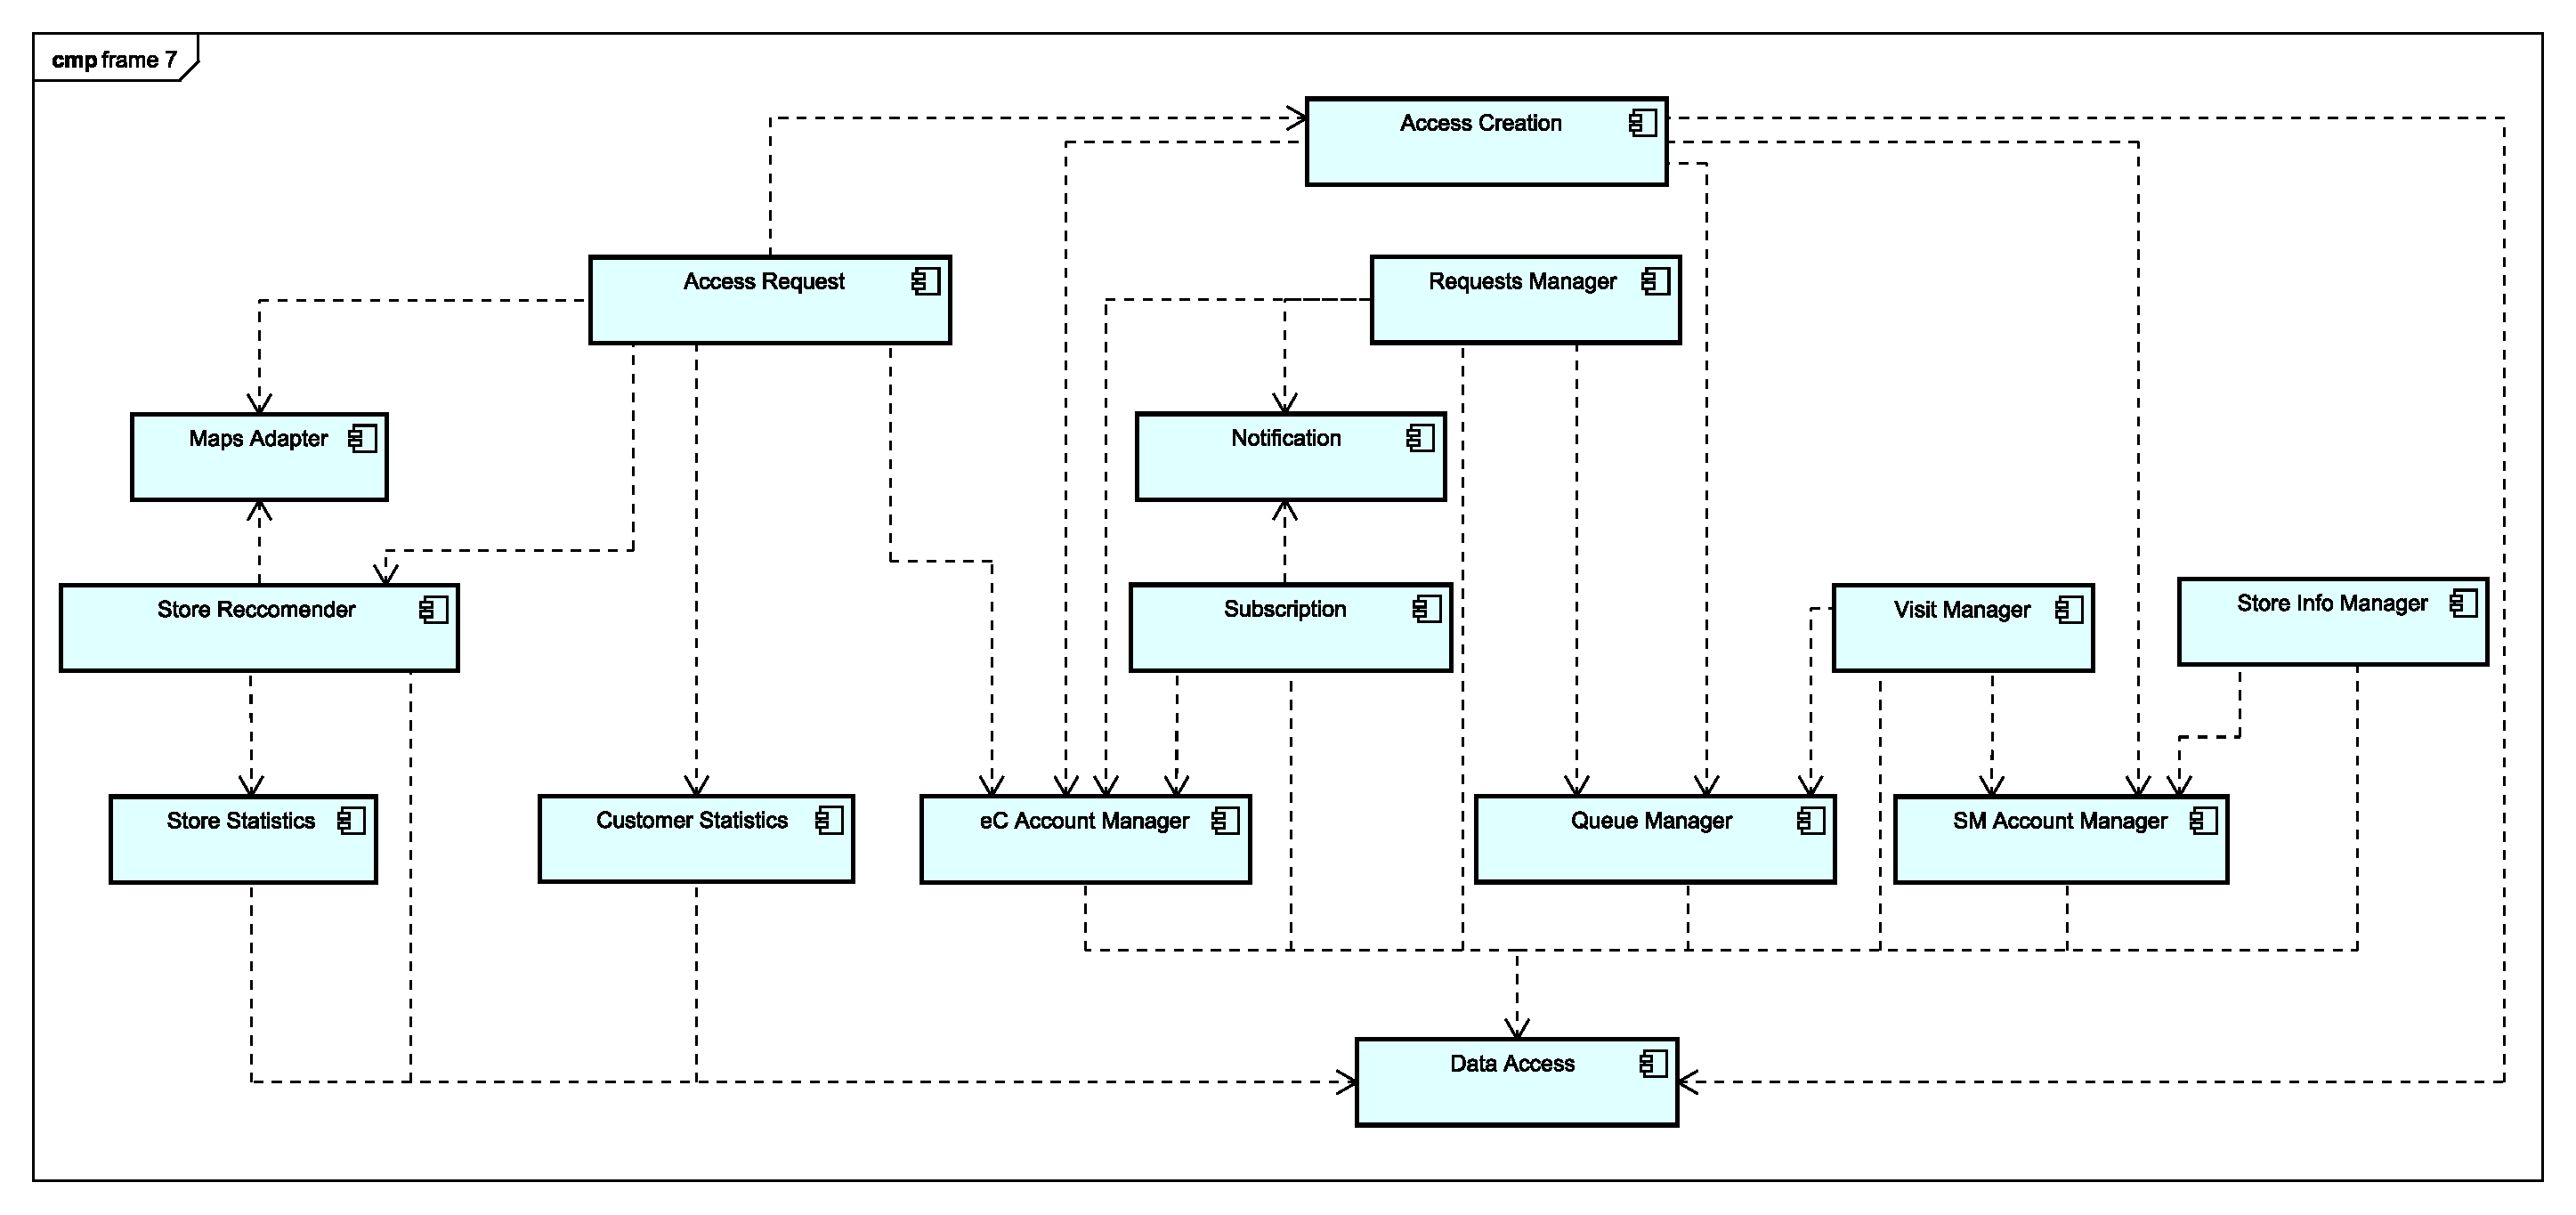
\includegraphics[width=\linewidth] {iit/frame_8}
	\caption{Final module integration with the previously missing Subscription Module}
	\label{frame_8} 
\end{figure}

\clearpage

\subsection{System Testing}
Once all the modules have been integrated, the system as whole should be tested for requirements satisfaction, both functional and non-functional.

\paragraph{Performance Testing}
Checking if the performance constraints defined in the RASD\textsuperscript{\cite{rasdperf}} are met is an important phase when testing the system as a whole. Moreover, it can help with the optimization of algorithms and queries (if helpful) and the identification of bottlenecks.

\paragraph{Load Testing}
This test should check that the system can handle the load defined in the previous document\textsuperscript{\cite{rasdperf}} and is fundamental to expose potential memory occupancy issues.

\paragraph{Stress Testing}
This final test type should test the ability of the system to handle failures and recover from them. 

\paragraph{Other tests}
After the system testing is successfully completed, an acceptance test can be done in order to assess the usability and the validity of the system. Finally, if the system is going to be used in an environment which is different from the developing one, and installation test can be carried out

	
	% Effort section
	\clearpage
	% Effort section, to be included in dd.tex

\section{Effort and tools}
\label{sect:effort}

\subsection{Effort spent breakdown}
\begin{center}
	\arrayrulecolor{tableborder}
	\setlength{\arrayrulewidth}{0.5mm}
	\rowcolors{0}{white}{tablerow}
	\begin{tabular}[width=\textwidth]{r | c c c | c}
		                          & 			  & 			   & 				& TOTAL \\ \hline
		Previous DD analysis      & 3.5           & 4              & 3              & 4.5   \\
		Hardware architecture     & 1             & 1              & 1              & 1     \\
		Component view            & 3.5           & 6.5            & 11.5           & 14.5  \\
		ER model                  & 4             & -              & 2              & 4     \\
		Document writing          & 14.5          & 4.5            & 5.5            & 14.5  \\
		UX design                 & -             & 3              & 3              & 5     \\
		Requirements traceability & 1.5           & 0.5            & 1.5            & 2.5   \\
		Deployment diagrams       & 1             & 4.5            & 4.5            & 4.5   \\
		Class diagram             & 2.5           & 2              & -              & 2.5   \\
		IIT	 					  & 4             & 6.5            & 6.5            & 6.5   \\
		Algorithm design          & 1             & 1              & 1              & 1     \\
		Sequence diagrams         & 2             & 5.5            & 1              & 5.5   \\
		Interface diagram         & 0.5           & 0.5            & 1.5            & 1.5   \\ \hline
		TOTAL                     & 39            & 39.5           & 42             & 67.5 
	\end{tabular}
\end{center}

\subsection{Software tools}
This is the list of tools used during the development of this document:
\begin{itemize}[itemsep=-1mm, topsep=-1mm]
	\item \textbf{\href{https://www.texstudio.org/}{TeXstudio}}: Text editor
	\item \textbf{\href{https://miktex.org/}{MikTeX}}: LaTeX compiler
	\item \textbf{\href{https://astah.net/}{Astah UML}}: UML modeling (class diagram, sequence diagrams, component diagrams, deployment diagram)
	\item \textbf{\href{https://draw.io/}{Draw.io}}: Other figures (ER model, hardware architecture, algorithms)
	\item \textbf{\href{https://pageloot.com/qr-code-generator/}{Pageloot}}: QR code generator for the algorithm
\end{itemize}
	
	% References and bibliography
	\clearpage
	\addcontentsline{toc}{section}{References}
	\bibliographystyle{plainurl}
	\bibliography{DD}
\end{document}
